\chapter{The Sensitivity of CLIC to Anomalous Gauge Couplings through Vector Boson Scattering}
\label{chap:PhysicsAnalysis}

\chapterquote{Kids, you tried your best, and you failed miserably.  The lesson is, never try.}%
{Homer Simpson}

\section{Background}
A potential source of beyond the standard model physics that could be studied at the CLIC experiment is that of the anomalous gauge couplings $\alpha_{4}$ and $\alpha_{5}$.  The theoretical basis for these couplings is described in section THEORY REF.  CLIC would show sensitivity to these couplings through vector boson scattering processes that are summarised in figures \ref{fig:vbsw}, \ref{fig:vbsz}, \ref{fig:vbswz} and \ref{fig:vbszw}.  An analysis of the sensitivity of CLIC to this processes is presented in the following chapter.

\iffalse

\begin{figure}
\begin{tikzpicture}[]
\begin{feynman}
\vertex (a1);
\vertex[above left=2cm of a1] (a2);
\vertex[above right=1cm and 2cm of a1] (a3) {\(W^{\pm},Z\)};
\vertex[below left=2cm of a1] (a4);
\vertex[below right=1cm and 2cm of a1] (a5) {\(W^{\mp},Z\)};
\vertex[above left=1cm of a2] (i1) {\(e^{-}\)};
\vertex[below left=1cm of a4] (i2) {\(e^{+}\)};
\vertex[above right=1cm and 3cm of a3] (i3) {\(q,l\)};
\vertex[below right=1cm and 3cm of a3] (i4) {\(\bar{q},\bar{l}\)};
\vertex[above right=1cm and 3cm of a5] (i5) {\(q,l\)};
\vertex[below right=1cm and 3cm of a5] (i6) {\(\bar{q},\bar{l}\)};
\vertex[above=1cm of a3] (v1) {\(\nu_{e}\)};
\vertex[below=1cm of a5] (v2) {\(\bar{\nu_{e}}\)};
\diagram* {
   (a1) -- [boson, edge label'=\(W^{-}\)] (a2) 
   (a1) -- [boson] (a3) 
   (a1) -- [boson, edge label=\(W^{+}\)] (a4) 
   (a1) -- [boson] (a5) 
   (i1) -- [fermion] (a2) -- [fermion] (v1)
   (v2) -- [fermion] (a4) -- [fermion] (i2)
   (i4) -- [fermion] (a3) -- [fermion] (i3)
   (i6) -- [fermion] (a5) -- [fermion] (i5)
};
\end{feynman}
\end{tikzpicture}
\caption[Feynman diagram of vector boson scattering at CLIC involving radiation of W bosons.]{Feynman diagram of vector boson scattering at CLIC involving radiation of W bosons.  $q = \text{u, d, s, b, c}$ and $l = \text{e, } \mu \text{, } \tau \text{, } \nu_{e} \text{, } \nu_{\nu} \text{, } \nu_{\tau}$}
\label{fig:vbsw}
\end{figure}

\begin{figure}
\begin{tikzpicture}[]
\begin{feynman}
\vertex (a1);
\vertex[above left=2cm of a1] (a2);
\vertex[above right=1cm and 2cm of a1] (a3) {\(W^{\pm},Z\)};
\vertex[below left=2cm of a1] (a4);
\vertex[below right=1cm and 2cm of a1] (a5) {\(W^{\mp},Z\)};
\vertex[above left=1cm of a2] (i1) {\(e^{-}\)};
\vertex[below left=1cm of a4] (i2) {\(e^{+}\)};
\vertex[above right=1cm and 3cm of a3] (i3) {\(q,l\)};
\vertex[below right=1cm and 3cm of a3] (i4) {\(\bar{q},\bar{l}\)};
\vertex[above right=1cm and 3cm of a5] (i5) {\(q,l\)};
\vertex[below right=1cm and 3cm of a5] (i6) {\(\bar{q},\bar{l}\)};
\vertex[above=1cm of a3] (v1) {\(e^{-}\)};
\vertex[below=1cm of a5] (v2) {\(e^{+}\)};
\diagram* {
   (a1) -- [boson, edge label'=\(Z\)] (a2)
   (a1) -- [boson] (a3)
   (a1) -- [boson, edge label=\(Z\)] (a4)
   (a1) -- [boson] (a5)
   (i1) -- [fermion] (a2) -- [fermion] (v1)
   (v2) -- [fermion] (a4) -- [fermion] (i2)
   (i4) -- [fermion] (a3) -- [fermion] (i3)
   (i6) -- [fermion] (a5) -- [fermion] (i5)
};
\end{feynman}
\end{tikzpicture}
\caption[Feynman diagram of vector boson scattering at CLIC involving radiation of Z bosons.]{Feynman diagram of vector boson scattering at CLIC involving radiation of Z bosons.  $q = \text{u, d, s, b, c}$ and $l = \text{e, } \mu \text{, } \tau \text{, } \nu_{e} \text{, } \nu_{\nu} \text{, } \nu_{\tau}$}
\label{fig:vbsz}
\end{figure}

\begin{figure}
\begin{tikzpicture}[]
\begin{feynman}
\vertex (a1);
\vertex[above left=2cm of a1] (a2);
\vertex[above right=1cm and 2cm of a1] (a3) {\(W^{-}\)};
\vertex[below left=2cm of a1] (a4);
\vertex[below right=1cm and 2cm of a1] (a5) {\(Z\)};
\vertex[above left=1cm of a2] (i1) {\(e^{-}\)};
\vertex[below left=1cm of a4] (i2) {\(e^{+}\)};
\vertex[above right=1cm and 3cm of a3] (i3) {\(q,l\)};
\vertex[below right=1cm and 3cm of a3] (i4) {\(\bar{q},\bar{l}\)};
\vertex[above right=1cm and 3cm of a5] (i5) {\(q,l\)};
\vertex[below right=1cm and 3cm of a5] (i6) {\(\bar{q},\bar{l}\)};
\vertex[above=1cm of a3] (v1) {\(\nu_{e}\)};
\vertex[below=1cm of a5] (v2) {\(e^{+}\)};
\diagram* {
   (a1) -- [boson, edge label'=\(W^{-}\)] (a2)
   (a1) -- [boson] (a3)
   (a1) -- [boson, edge label=\(Z\)] (a4)
   (a1) -- [boson] (a5)
   (i1) -- [fermion] (a2) -- [fermion] (v1)
   (v2) -- [fermion] (a4) -- [fermion] (i2)
   (i4) -- [fermion] (a3) -- [fermion] (i3)
   (i6) -- [fermion] (a5) -- [fermion] (i5)
};
\end{feynman}
\end{tikzpicture}
\caption[Feynman diagram of vector boson scattering at CLIC involving radiation of Z bosons.]{Feynman diagram of vector boson scattering at CLIC involving radiation of a W and Z boson.  $q = \text{u, d, s, b, c}$ and $l = \text{e, } \mu \text{, } \tau \text{, } \nu_{e} \text{, } \nu_{\nu} \text{, } \nu_{\tau}$}
\label{fig:vbswz}
\end{figure}

\begin{figure}
\begin{tikzpicture}[]
\begin{feynman}
\vertex (a1);
\vertex[above left=2cm of a1] (a2);
\vertex[above right=1cm and 2cm of a1] (a3) {\(Z\)};
\vertex[below left=2cm of a1] (a4);
\vertex[below right=1cm and 2cm of a1] (a5) {\(W^{+}\)};
\vertex[above left=1cm of a2] (i1) {\(e^{-}\)};
\vertex[below left=1cm of a4] (i2) {\(e^{+}\)};
\vertex[above right=1cm and 3cm of a3] (i3) {\(q,l\)};
\vertex[below right=1cm and 3cm of a3] (i4) {\(\bar{q},\bar{l}\)};
\vertex[above right=1cm and 3cm of a5] (i5) {\(q,l\)};
\vertex[below right=1cm and 3cm of a5] (i6) {\(\bar{q},\bar{l}\)};
\vertex[above=1cm of a3] (v1) {\(e^{-}\)};
\vertex[below=1cm of a5] (v2) {\(\bar{\nu_{e}}\)};
\diagram* {
   (a1) -- [boson, edge label'=\(Z\)] (a2)
   (a1) -- [boson] (a3)
   (a1) -- [boson, edge label=\(W^{+}\)] (a4)
   (a1) -- [boson] (a5)
   (i1) -- [fermion] (a2) -- [fermion] (v1)
   (v2) -- [fermion] (a4) -- [fermion] (i2)
   (i4) -- [fermion] (a3) -- [fermion] (i3)
   (i6) -- [fermion] (a5) -- [fermion] (i5)
};
\end{feynman}
\end{tikzpicture}
\caption[Feynman diagram of vector boson scattering at CLIC involving radiation of Z bosons.]{Feynman diagram of vector boson scattering at CLIC involving radiation of a W and Z boson.  $q = \text{u, d, s, b, c}$ and $l = \text{e, } \mu \text{, } \tau \text{, } \nu_{e} \text{, } \nu_{\nu} \text{, } \nu_{\tau}$}
\label{fig:vbszw}
\end{figure}

\fi

\section{Generation}
\label{sec:eventgenerationandbackgrounds}
The event generation software used by the CLIC experiment is Whizard \cite{0708.4233, hep-ph/0102195}.  Whizard version 1.97 was used for generating the new samples, while version 1.95 is used for the official CLIC samples. It was recommended by the Whizard authors to use version 1.97 as it contains a unitarisation scheme that ensures the probabilities remain physical up to high energies when considering the effect of anomalous gauge couplings.  

The hadronic channels are the dominant decay modes of the W and the Z boson, with branching fractions of the order of 70\% for both (REFERENCE PDG), and as the vector boson scattering is the desired signal channel, the focus of this analysis will be upon the hadronic decays of the W and Z.  The vector boson scattering dominated signal final states containing hadronic decay products for the bosons are $\nu\nu\text{qqqq}$, $\text{l}\nu\text{qqqq}$ and llqqqq.  

\subsection{Cross Section Sensitivity}
\label{sec:crosssectioncheck}
To determine which final states are sensitive to $\alpha_{4}$ and $\alpha_{5}$ a comparison was made between the cross section using the standard model values of $\alpha_{4}$ and $\alpha_{5}$, i.e. 0, and the same calculation using non-zero values of these couplings.  This comparison was performed on all final states that would be relevant either as signal or background processes, for an analysis involving the purely hadronic decay channels of a vector boson scattering process.  In full the states that were tested are:

\begin{itemize}
\item Vector boson scattering signal final states that are expected to show sensitivity to the anomalous couplings: $\text{e}^{+}\text{e}^{-} \rightarrow \nu\nu\text{qqqq}$, $\text{e}^{+}\text{e}^{-} \rightarrow \text{l}\nu\text{qqqq}$ and $\text{e}^{+}\text{e}^{-} \rightarrow \text{llqqqq}$
\item Four jet final states arising from $\text{e}^{+}\text{e}^{-}$ interactions: $\text{e}^{+}\text{e}^{-} \rightarrow \text{qqqq}$.
\item Two jet final states arising from $\text{e}^{+}\text{e}^{-}$ interactions: $\text{e}^{+}\text{e}^{-} \rightarrow \nu{\nu}\text{qq}$, $\text{e}^{+}\text{e}^{-} \rightarrow \text{l}\nu\text{qq}$, $\text{e}^{+}\text{e}^{-} \rightarrow \text{llqq}$ and $\text{e}^{+}\text{e}^{-} \rightarrow \text{qq}$.
\item Four jet final states arising from the interactions of either $\text{e}^{+}$ or $\text{e}^{-}$ with a beamstrahlung photon: $\gamma_{\text{BS}}\text{e}^{-} \rightarrow \text{qqqq}\text{e}^{-}$, $\text{e}^{+}\gamma_{\text{BS}} \rightarrow \text{qqqq}\text{e}^{+}$, $\gamma_{\text{BS}}\text{e}^{-} \rightarrow \text{qqqq}\nu$ and $\text{e}^{+}\gamma_{\text{BS}} \rightarrow \text{qqqq}\nu$.
\item Four jet final states arising from the interactions of either $\text{e}^{+}$ or $\text{e}^{-}$ with the electromagnetic field of the opposing beam particle.  These cross sections are calculated using equivalent photon approximation (EPA), which represents the electromagnetic field of the opposing beam particle as a series of photon and so the final states appear as interactions of $\text{e}^{+}$ or $\text{e}^{-}$ with photons: $\gamma_{\text{EPA}}\text{e}^{-} \rightarrow \text{qqqq}\text{e}^{-}$, $\text{e}^{+}\gamma_{\text{EPA}} \rightarrow \text{qqqq}\text{e}^{+}$, $\gamma_{\text{EPA}}\text{e}^{-} \rightarrow \text{qqqq}\nu$ and $\text{e}^{+}\gamma_{\text{EPA}} \rightarrow \text{qqqq}\nu$.
\item Four jet final states arising from the interaction of the electromagnetic fields of opposing beam particles using the EPA approximation: $\gamma_{\text{EPA}}\gamma_{\text{EPA}} \rightarrow \text{qqqq}$.
\item Four jet final states arising from the interaction of the electromagnetic field of either $\text{e}^{+}$ or $\text{e}^{-}$ using the EPA approximation with a beamstrahlung photon: $\gamma_{\text{EPA}}\gamma_{\text{BS}} \rightarrow \text{qqqq}$ or $\gamma_{\text{BS}}\gamma_{\text{EPA}} \rightarrow \text{qqqq}$.
\item Four jet final states arising from the interaction of two beamstrahlung photons: $\gamma_{\text{BS}}\gamma_{\text{BS}} \rightarrow \text{qqqq}$.
\end{itemize}

Note: In the above list q = u, d, s, c and b, l = e, $\mu$, $\tau$ and $\nu$ = $\nu_{e}$, $\nu_{\mu}$ and $\nu_{\tau}$.

The cross section was found to differ when using non-zero values for the anomalous couplings in comparison to the standard model prediction for the vector boson scattering signal final states $\nu\nu\text{qqqq}$, $\text{l}\nu\text{qqqq}$ and llqqqq.  The cross section comparisons for these final states can be found in table \ref{table:crosssectionsensitivity1400} and table \ref{table:crosssectionsensitivity3000} for 1.4 and 3 TeV samples respectively.  In reality, non-zero anomalous couplings would change the cross sections of all processes considered, however, the sensitivity would only arise from high order terms in the Lagrangian.  Such terms would not be dominant in determining the cross section and so are omitted from the generator making certain final states appear invariant to changes in the anomalous couplings.

\begin{table}[h!]
\centering
\begin{tabular}{ l l l l l}
\hline
Final State & Cross Section [fb] & Cross Section [fb] & Percentage & CLIC Cross Section \\ 
& ($\alpha_{4} = \alpha_{5} = 0.00$) & ($\alpha_{4} = \alpha_{5} = 0.05$) & Change[\%] & [fb] \\ 
\hline
$\text{e}^{+}\text{e}^{-} \rightarrow \nu{\nu}\text{qqqq}$ & 20.8 & 34.6 & +66.3 & 24.7 \\
$\text{e}^{+}\text{e}^{-} \rightarrow \text{l}{\nu}\text{qqqq}$ & 112 & 113 & +0.9 & 115.3 \\
$\text{e}^{+}\text{e}^{-} \rightarrow \text{llqqqq}$ & 59.7 & 68.6 & +14.9 & 62.1 \\
\hline
\end{tabular}
\caption{Cross section for selected processes for given value of $\alpha_{4}$ and $\alpha_{5}$ at 1.4 TeV.}
\label{table:crosssectionsensitivity1400}

\begin{tabular}{ l l l l l}
\hline
Final State & Cross Section [fb] & Cross Section [fb] & Percentage & CLIC Cross Section \\ 
& ($\alpha_{4} = \alpha_{5} = 0.000$) & ($\alpha_{4} = \alpha_{5} = 0.005$) & Change[\%] & [fb] \\ 
\hline
$\text{e}^{+}\text{e}^{-} \rightarrow \nu{\nu}\text{qqqq}$ & 51.2 & 77.7 & +51.8 & 71.5 \\
$\text{e}^{+}\text{e}^{-} \rightarrow \text{l}{\nu}\text{qqqq}$ & 111.9 & 115.9 & +3.6 & 106.6 \\
$\text{e}^{+}\text{e}^{-} \rightarrow \text{llqqqq}$ & 169.7 & 161.7 & -4.9 & 169.3 \\
\hline
\end{tabular}
\caption{Cross section for selected processes for given value of $\alpha_{4}$ and $\alpha_{5}$ at 3 TeV.}
\label{table:crosssectionsensitivity3000}
\end{table}

The cross section calculations show that the most sensitive final state to the anomalous gauge couplings is \nu{\nu}qqqq, therefore, this analysis will focus solely upon this final state.  Furthermore, as the l{\nu}qqqq final state has a much reduced sensitivity in comparison to the \nu{\nu}qqqq state and as the llqqqq can be easily vetoed from the analysis, as will be shown in subsequent chapters, it is only necessary to consider the sensitivity of the \nu{\nu}qqqq final state.  For the aforementioned reasons the l{\nu}qqqq and llqqqq final states will be treated as backgrounds that are invariant to changes in the anomalous couplings $\alpha_{4}$ and $\alpha_{5}$.  

\subsection{Event Weights}
The sensitivity of an individual event to the anomalous gauge couplings is determined through an event weight. This weight is given by the ratio of the squares of the matrix element used in the cross section calculation, one matrix element using non-zero values of $\alpha_{4}$ and $\alpha_{5}$ and the other matrix element using the standard model values of $\alpha_{4}$ and $\alpha_{5}$, i.e. 0.  The weight varies as a function of $\alpha_{4}$ and $\alpha_{5}$ as well as varying on an event by event basis as the kinematics of the final state changes.  Examples of the event weights as a function of $\alpha_{4}$ and $\alpha_{5}$ for selected events is shown in figure \ref{fig:eventweights1400raw} for 1.4 TeV events.

\begin{figure}
\centering
\subfloat[]{\label{fig:weight1}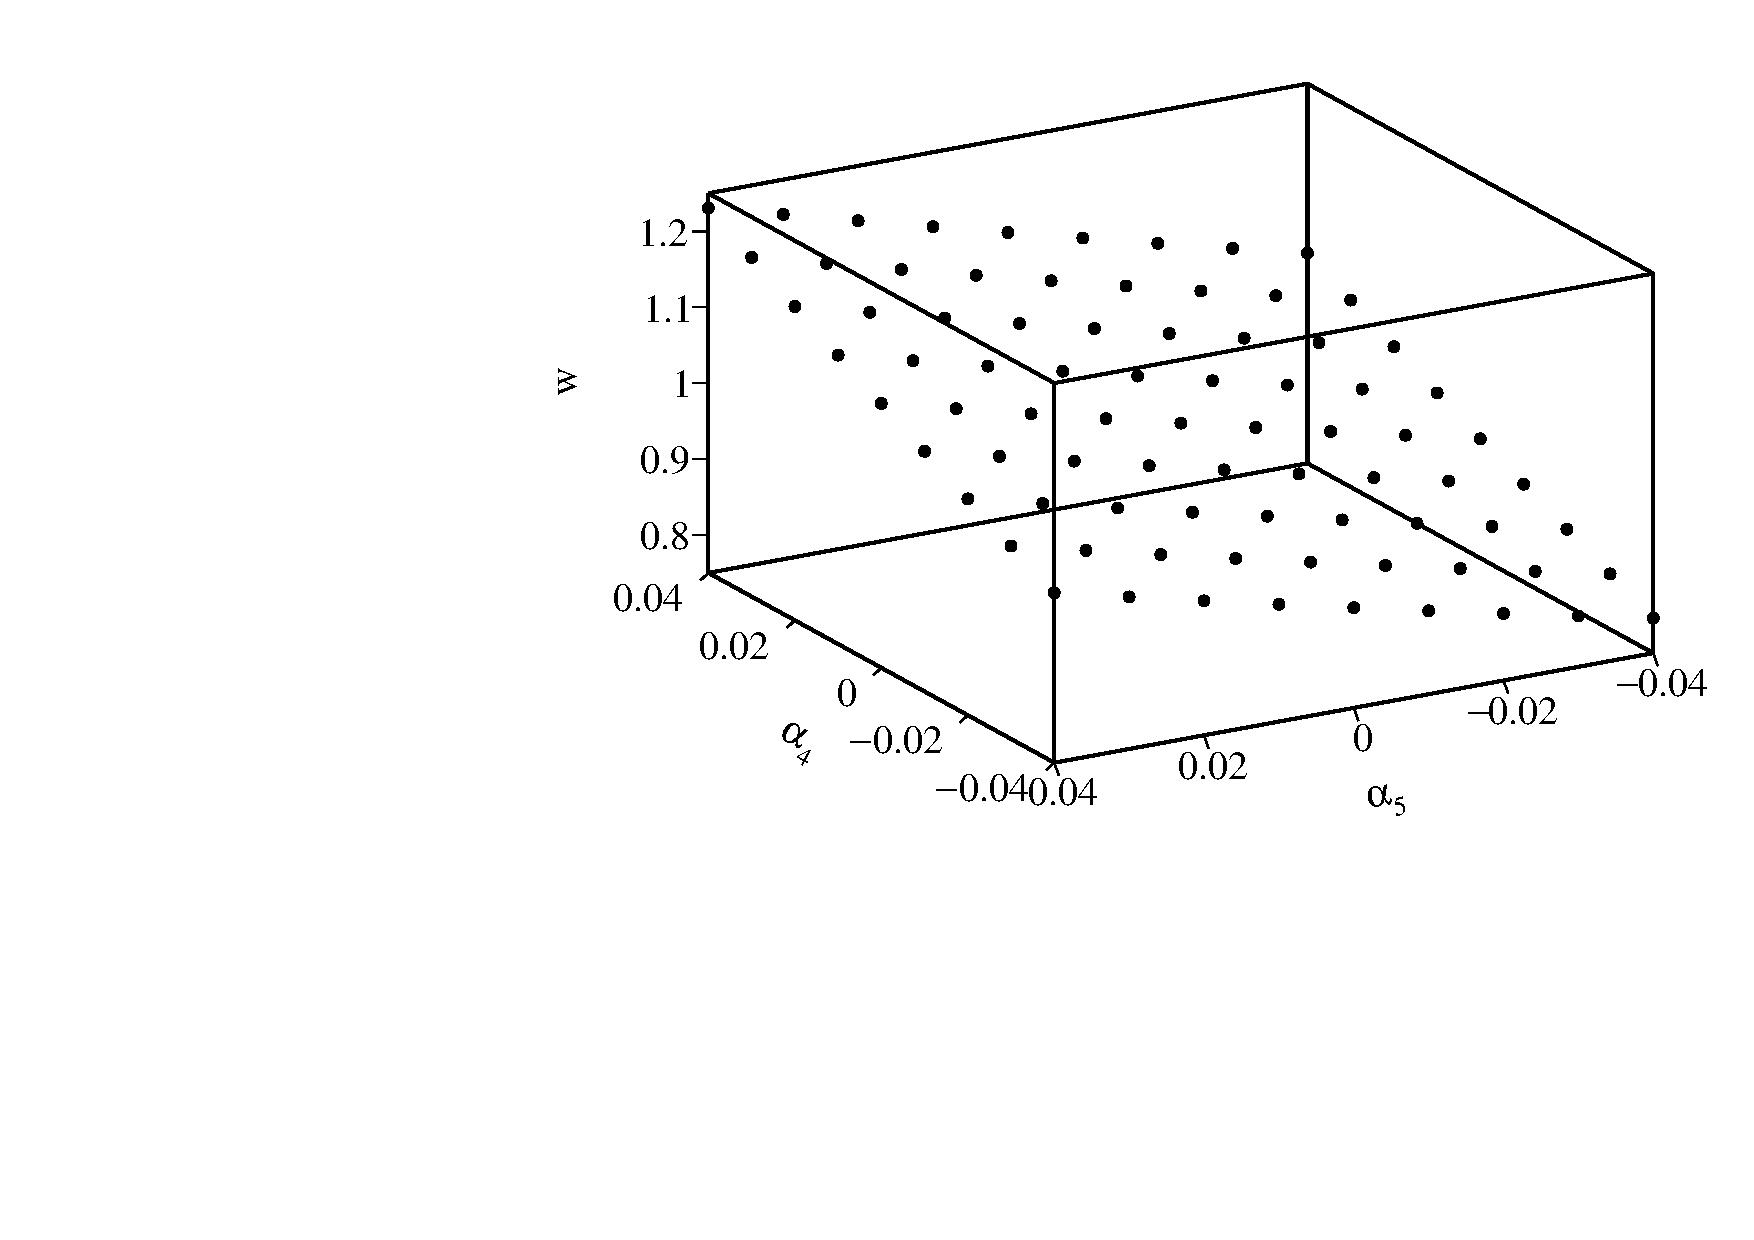
\includegraphics[width=0.5\textwidth]{PhysicsAnalysis/Plots/EventWeights/1400GeV/EventWeightsForEvent100001009_1400GeV_SPFOs_kt_0p70_10Bins_Start_0_End_10_1400GeV_Raw.pdf}}
\subfloat[]{\label{fig:weight2}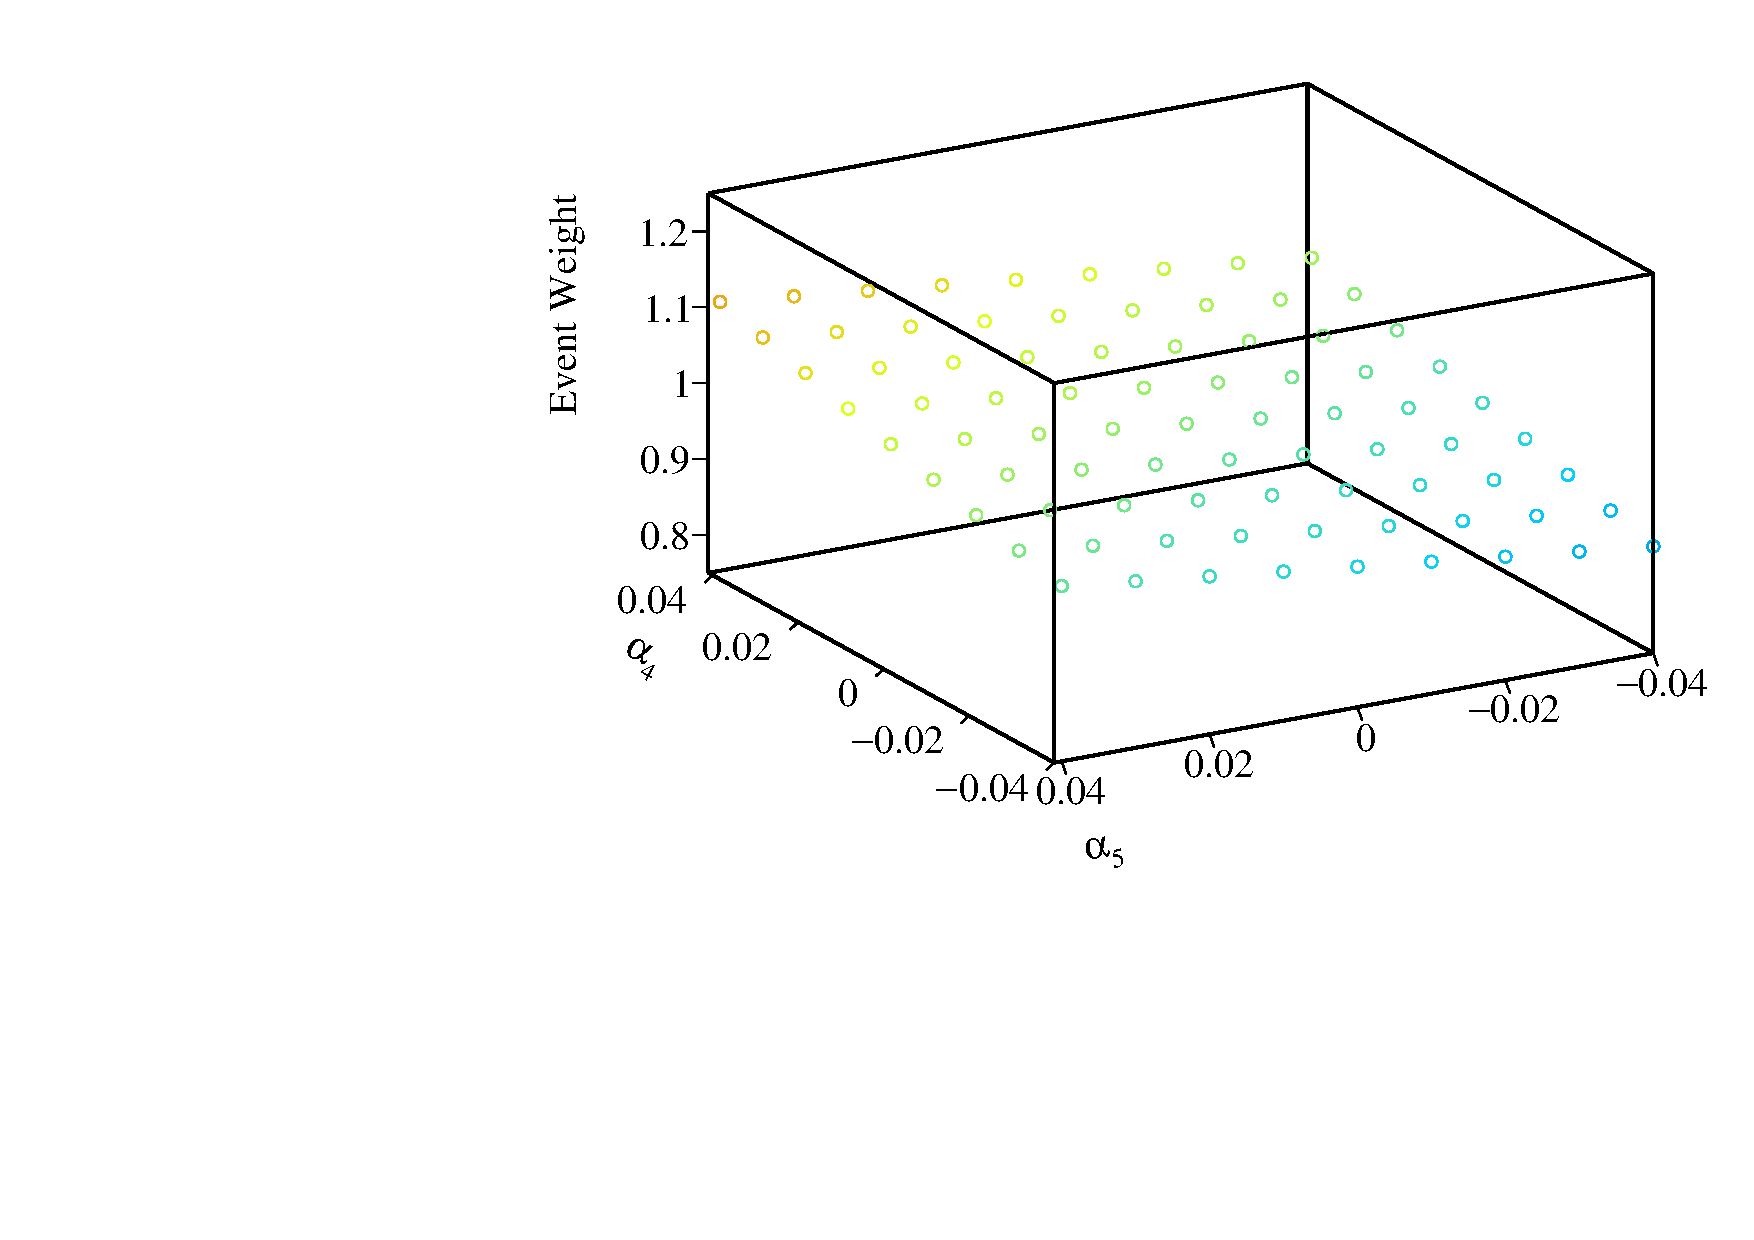
\includegraphics[width=0.5\textwidth]{PhysicsAnalysis/Plots/EventWeights/1400GeV/EventWeightsForEvent100001014_1400GeV_SPFOs_kt_0p70_10Bins_Start_0_End_10_1400GeV_Raw.pdf}} \hfill
\subfloat[]{\label{fig:weight3}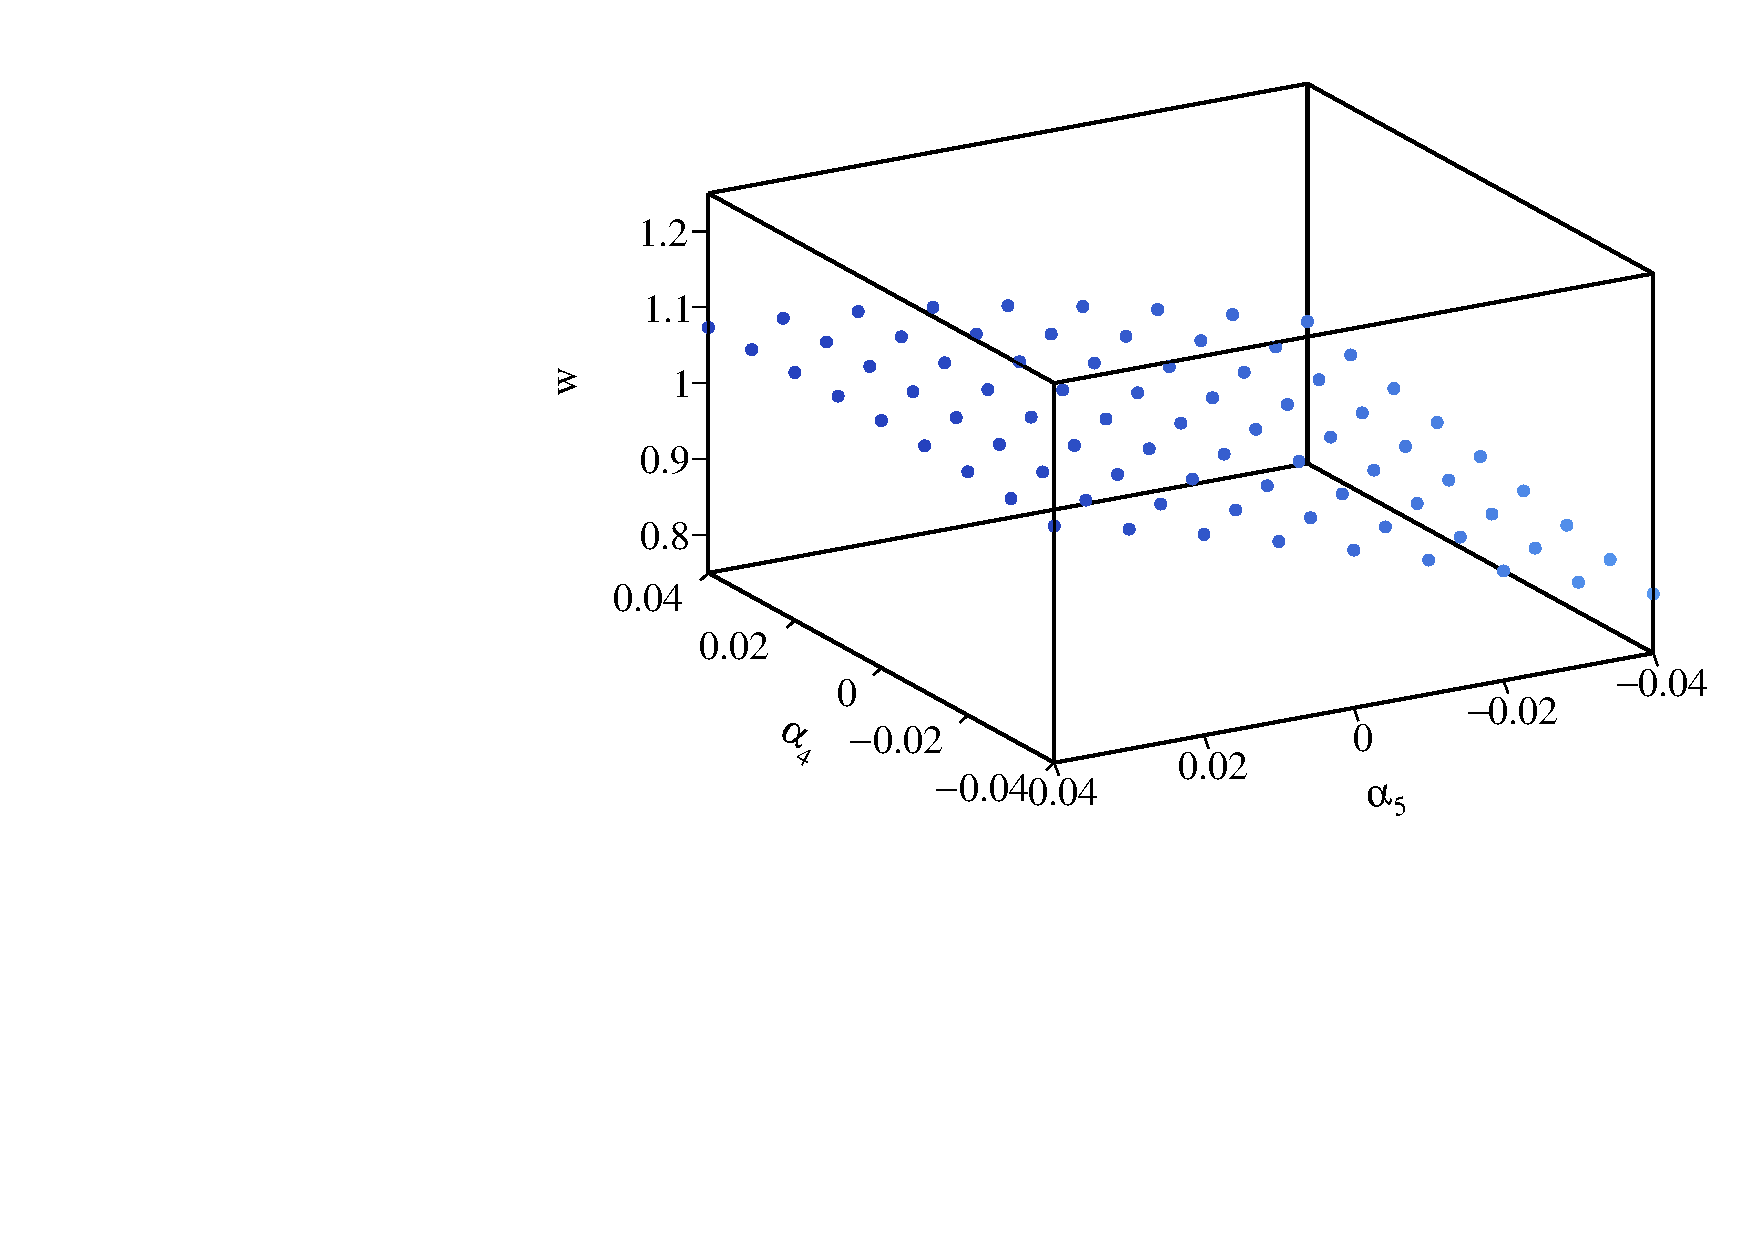
\includegraphics[width=0.5\textwidth]{PhysicsAnalysis/Plots/EventWeights/1400GeV/EventWeightsForEvent100001044_1400GeV_SPFOs_kt_0p70_10Bins_Start_0_End_10_1400GeV_Raw.pdf}}
\subfloat[]{\label{fig:weight4}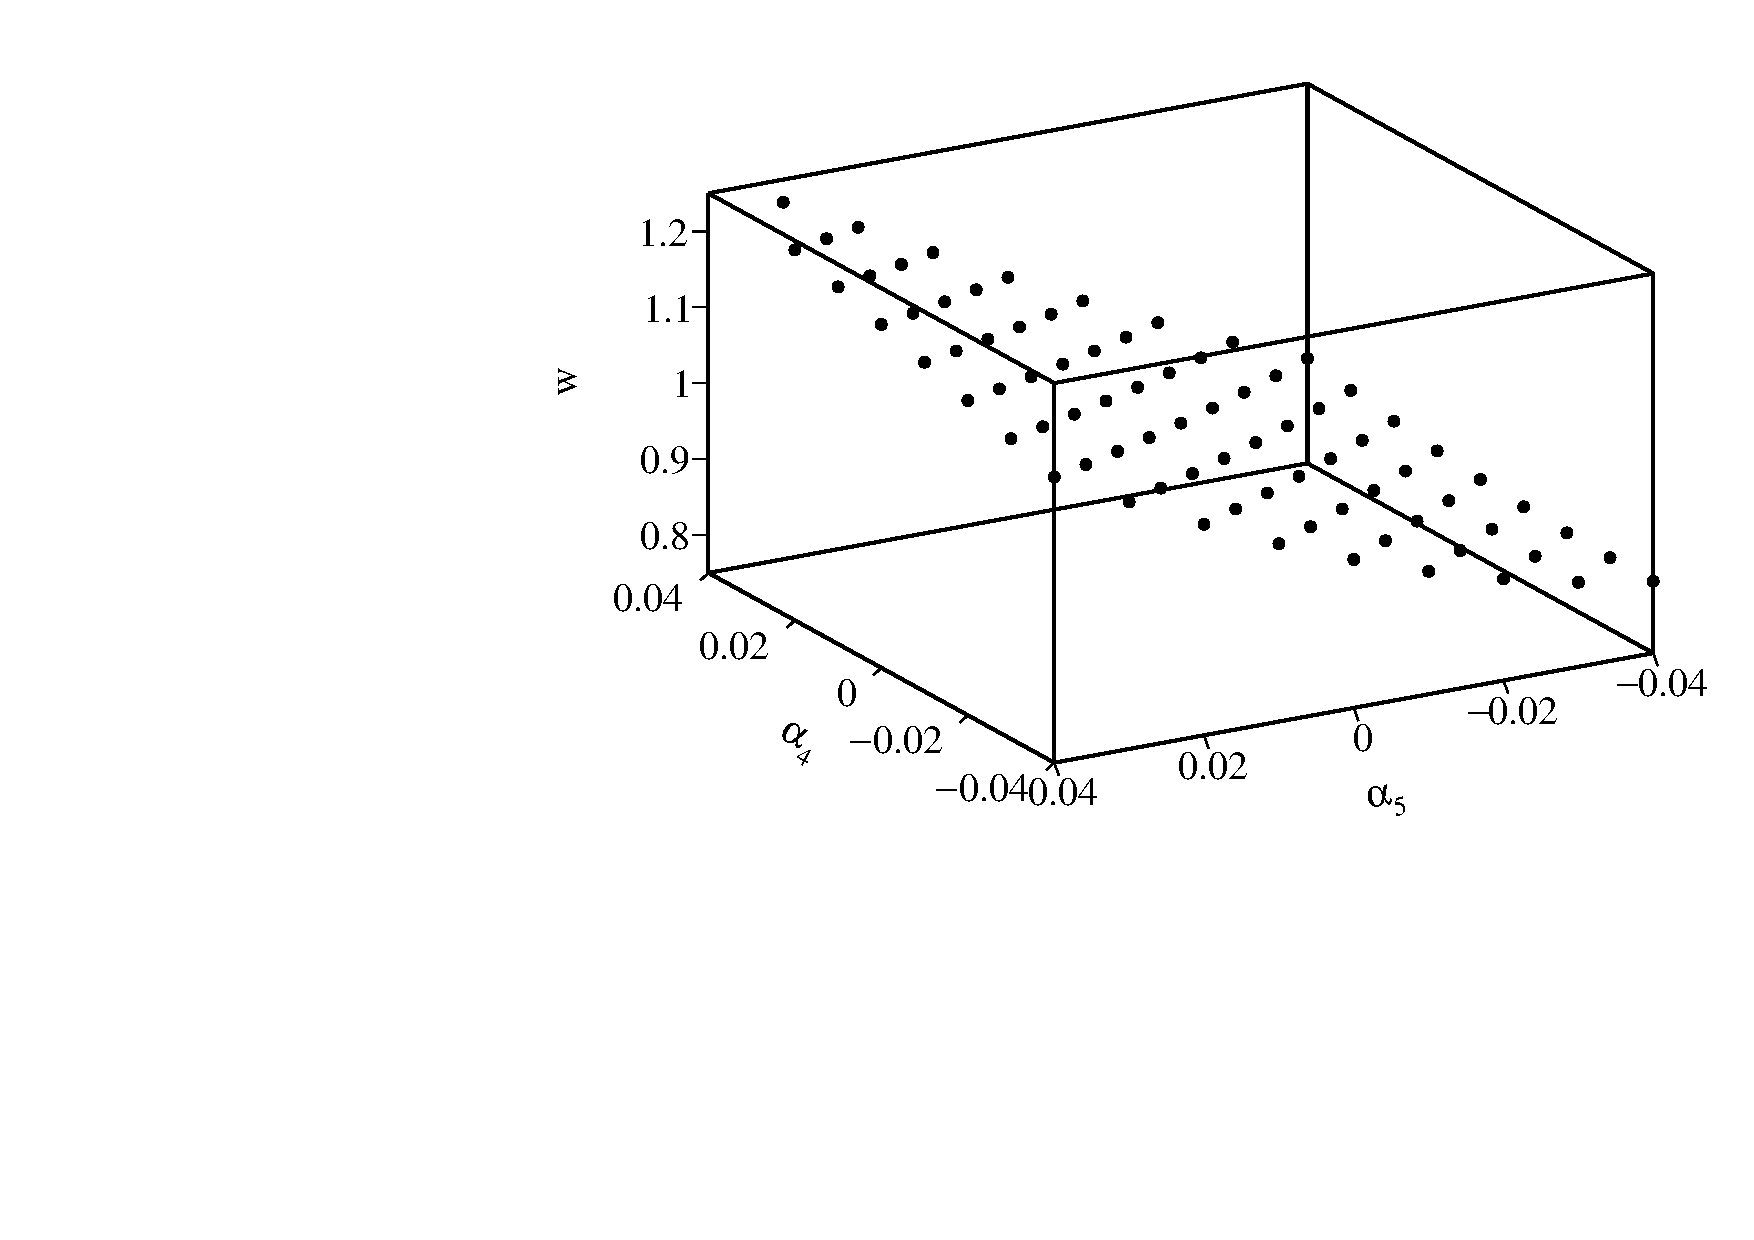
\includegraphics[width=0.5\textwidth]{PhysicsAnalysis/Plots/EventWeights/1400GeV/EventWeightsForEvent100001051_1400GeV_SPFOs_kt_0p70_10Bins_Start_0_End_10_1400GeV_Raw.pdf}}
\caption[Event weights from Whizard for 1.4TeV \nu{\nu}qqqq final state events.]{A selection of plots showing how the event weight changes when varying the anomalous couplings $\alpha_{4}$ and $\alpha_{5}$ for 1.4TeV \nu{\nu}qqqq final state events.}
\label{fig:eventweights1400raw}
\end{figure}

This reweighting procedure has many advantages over the alternative of generating new samples with fixed $\alpha_{4}$ and $\alpha_{5}$, notably the absence of systematic errors arising from new event generation, simulation and reconstruction.  

\subsection{Validation of Samples}
\label{sec:validationofsamples}
The CLIC experiment has a repository of simulated and reconstructed samples that can be used for physics analyses, however, it is not possible to calculate the event weights for these samples as the raw Whizard format event files are missing.  Therefore, a new $\text{e}^{+}\text{e}^{-} \rightarrow \nu\nu\text{qqqq}$ sample was generated with the relevant files to make reweighting as a function of $\alpha_{4}$ and $\alpha_{5}$ possible.  An identical setup to that used for the production of official CLIC samples was used for the event generation, detector simulation and reconstruction.  Mimicking this production chain made it possible to use the official CLIC samples for the background final states used in this analysis.  

Several reconstructed level distributions were compared to the official CLIC samples and were found to be comparable to each other. A selection of these distributions is shown in figure \ref{fig:cliccomp}.

In order to determine the event weights it was necessary to use the anomalous gauge coupling model in Whizard, which in turn enforces a unit CKM matrix.  In the context of vector boson scattering this will restrict the hadronic decays of the $\text{W}^{-}$ boson to d$\bar{\text{u}}$ and s$\bar{\text{c}}$, the $\text{W}^{+}$ boson to u$\bar{\text{d}}$ and c$\bar{\text{s}}$ and the Z boson to u$\bar{\text{u}}$ , d$\bar{\text{d}}$, s$\bar{\text{s}}$, c$\bar{\text{c}}$ and b$\bar{\text{b}}$.  In contrast the official CLIC samples use a non-unit CKM matrix, which gives rise to alternative hadronic decay modes for the W and Z bosons.  When comparing the unit CKM matrix and the non-unit CKM $\nu\nu\text{qqqq}$ final state samples it was found that there were negligible differences in a variety of reconstructed level distributions, such as those found in figure \ref{fig:cliccomp}.  Furthermore, as flavour tagging information is not used in this analysis this difference was deemed insignificant.  

\begin{figure}
\centering
\subfloat[Visible Mass, 1.4 TeV]{\label{fig:cliccomp1400_1}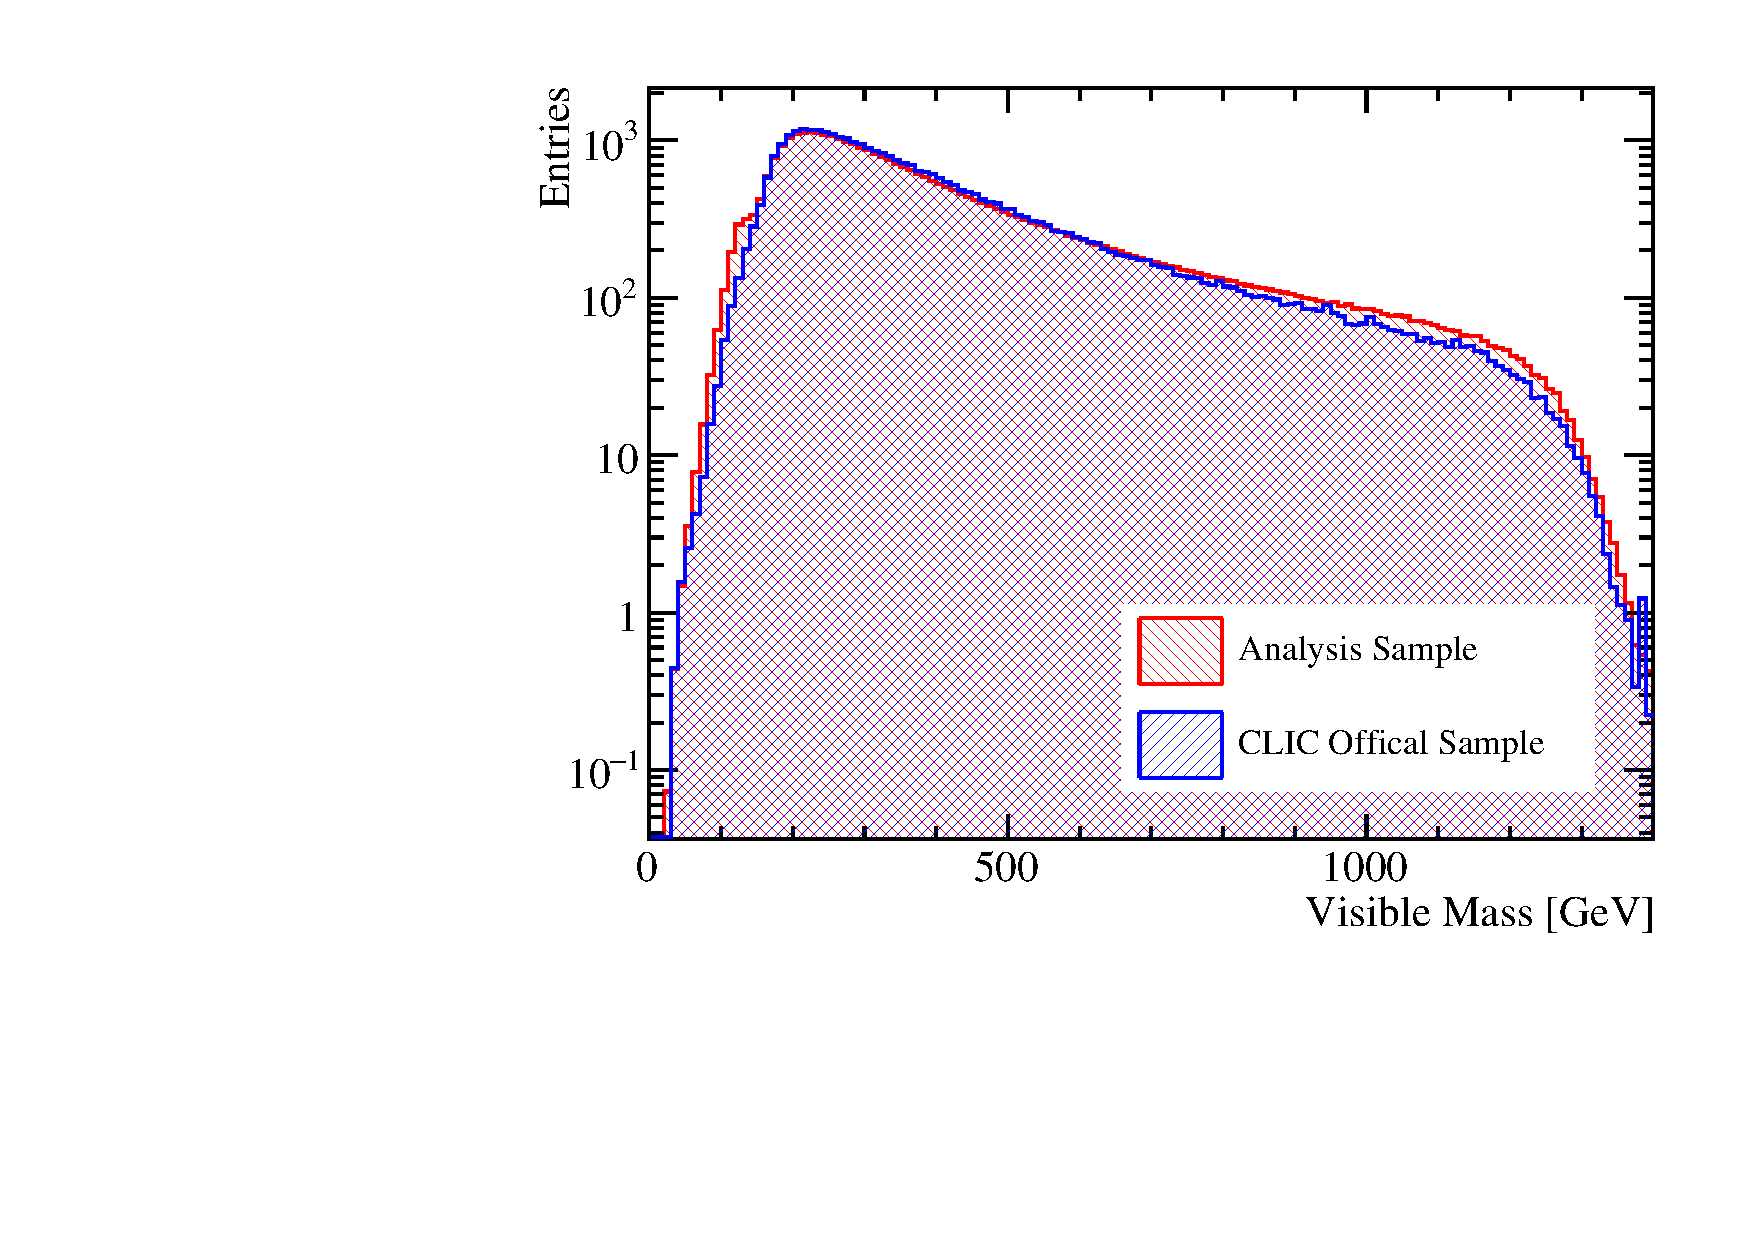
\includegraphics[width=0.5\textwidth]{PhysicsAnalysis/Plots/CLICSampleComparison/1400GeV/InvariantMassSystem.pdf}}
\subfloat[Visible Mass, 3 TeV]{\label{fig:cliccomp3000_1}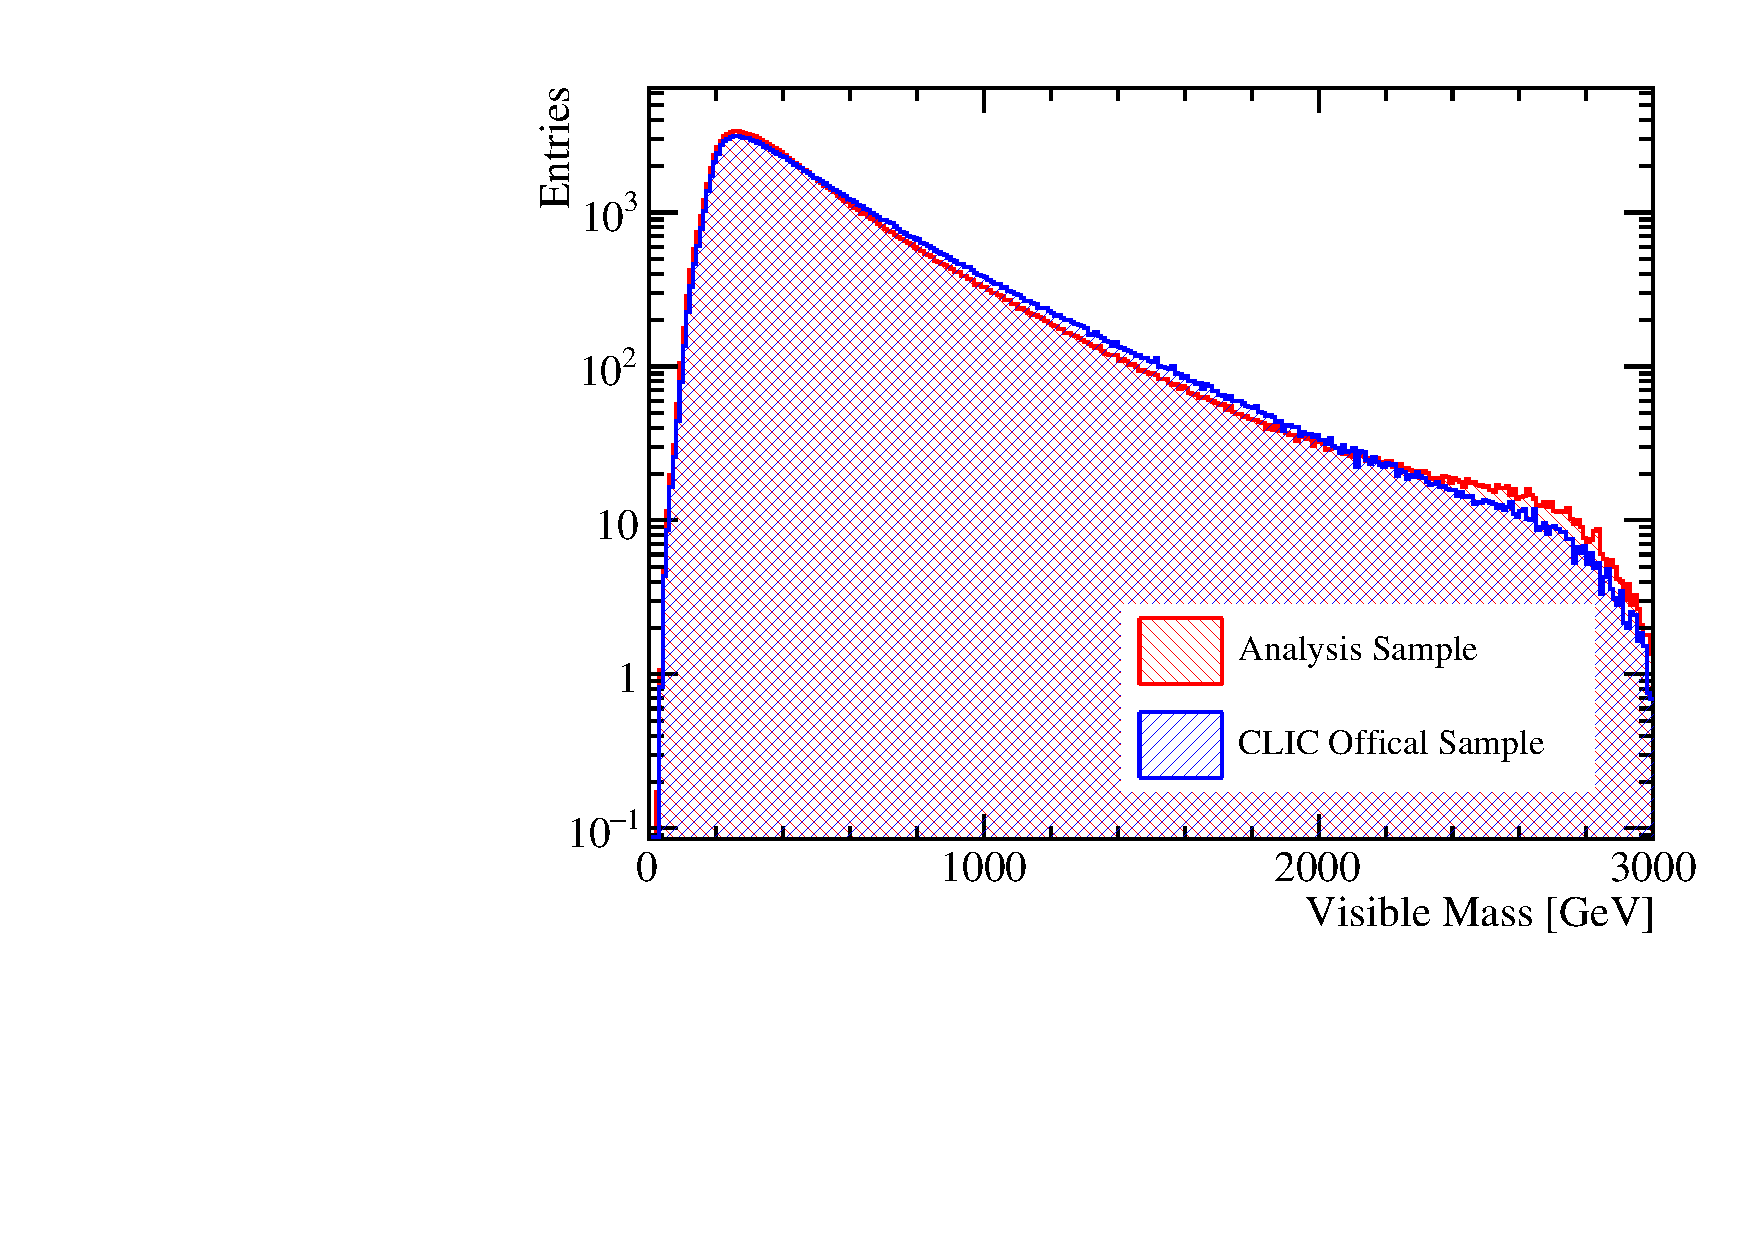
\includegraphics[width=0.5\textwidth]{PhysicsAnalysis/Plots/CLICSampleComparison/3000GeV/InvariantMassSystem.pdf}} \hfill
\subfloat[$\text{cos}\theta_{Missing}$ - The cosine of the polar angle of the missing momentum for an event, 1.4 TeV.]{\label{fig:cliccomp1400_2}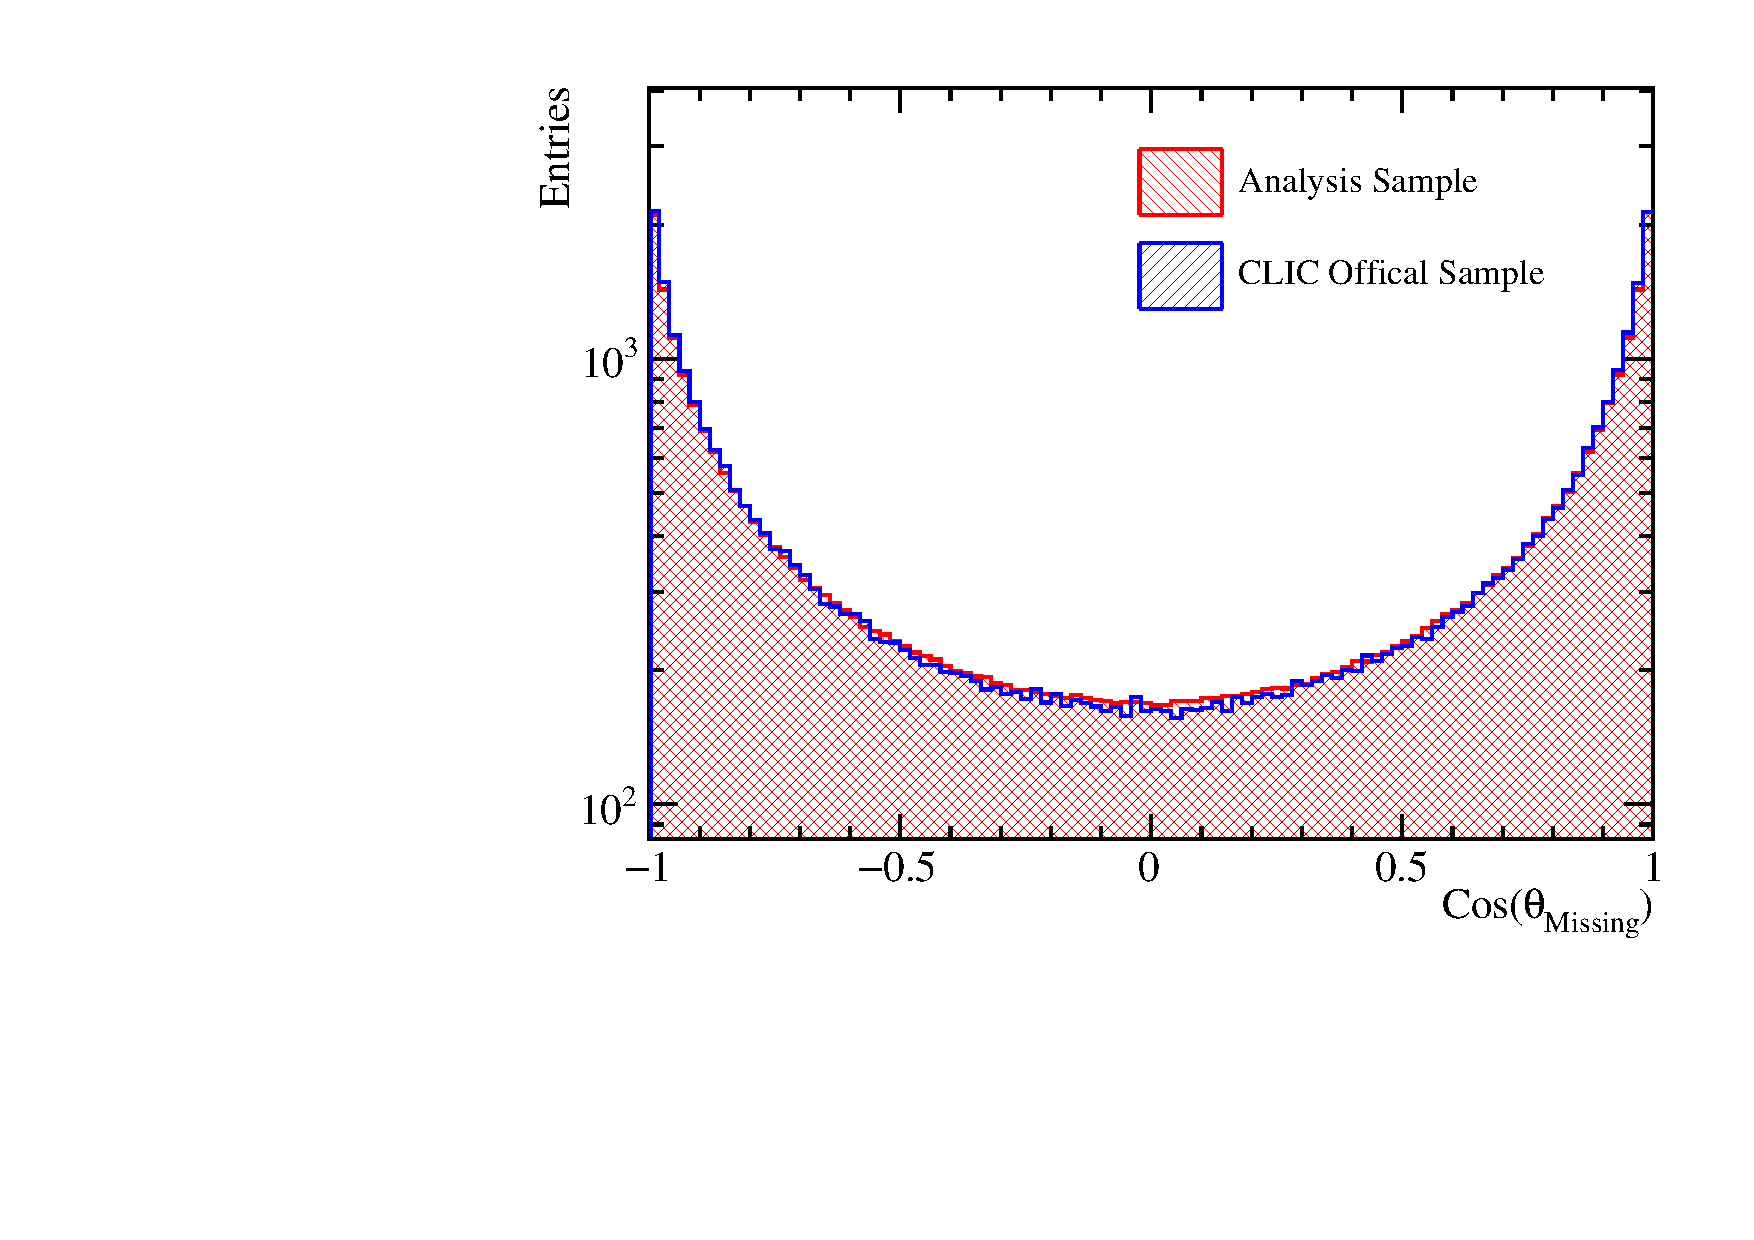
\includegraphics[width=0.5\textwidth]{PhysicsAnalysis/Plots/CLICSampleComparison/1400GeV/CosThetaMissing.pdf}} 
\subfloat[$\text{cos}\theta_{Missing}$ - The cosine of the polar angle of the missing momentum for an event, 3 TeV.]{\label{fig:cliccomp3000_2}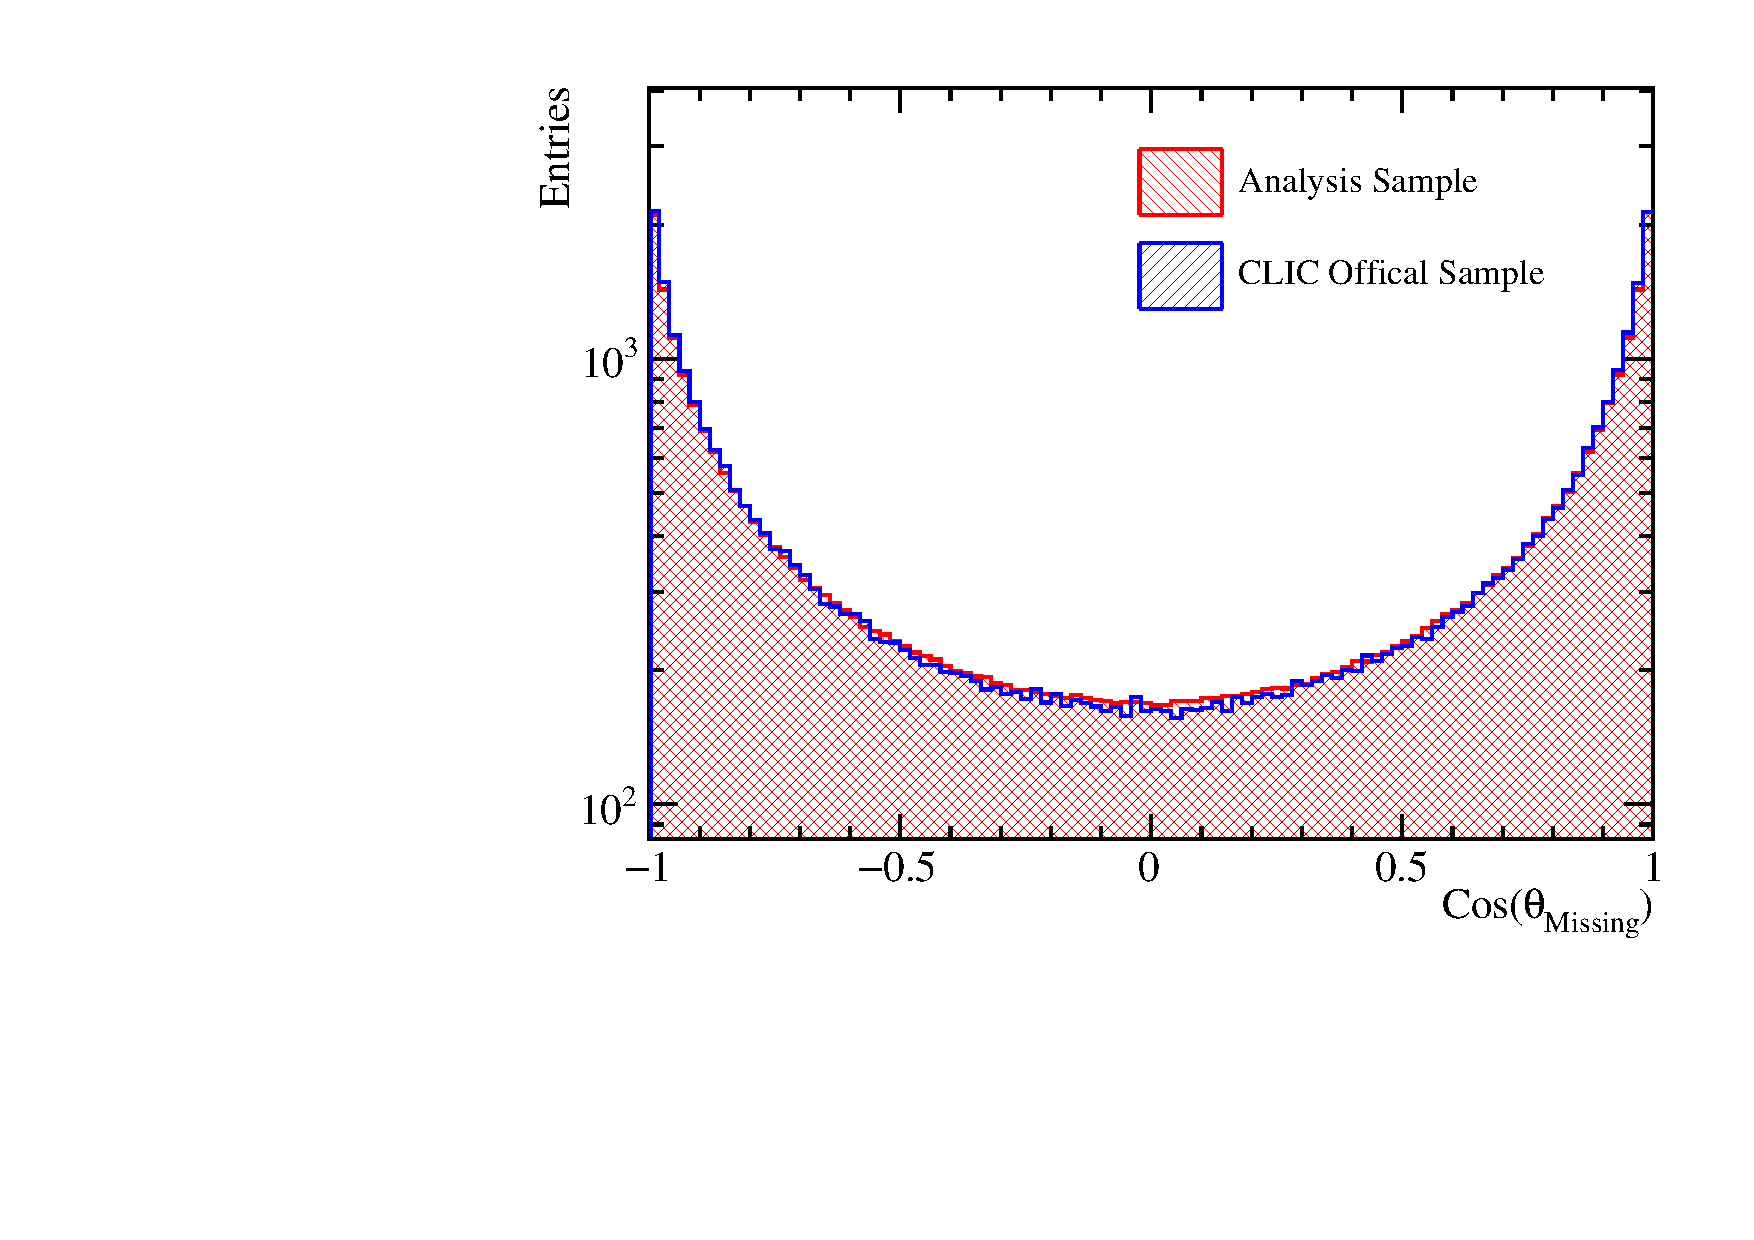
\includegraphics[width=0.5\textwidth]{PhysicsAnalysis/Plots/CLICSampleComparison/1400GeV/CosThetaMissing.pdf}} 
\caption[Comparison of various distributions between samples used in this analysis and the official CLIC samples for the \nu{\nu}qqqq final state at 1.4 and 3 TeV.]{Comparison of various distributions between samples used in this analysis and the official CLIC samples for the \nu{\nu}qqqq final state at 1.4 and 3 TeV.  Both samples have been normalised to the correct luminosity for CLIC running at the relevant energies TeV.}
\label{fig:cliccomp}
\end{figure}

\section{Simulation and Reconstruction}
For all samples considered in this analysis, the CLID\_ILD detector \cite{arXiv:1006.3396} was used.  The detector was simulated using MOKKA \cite{MoradeFreitas:2002kj}, a GEANT4 \cite{Agostinelli:2002hh} wrapper providing detailed geometric descriptions of detector concepts for the linear collider.  Events were reconstructed using MARLIN \cite{Gaede:2006pj}, a c++ framework designed for reconstruction at the linear collider.  PandoraPFA \cite{arXiv:0907.3577, arXiv:1209.4039} is used to apply particle flow calorimetry in this reconstruction.
 
The CLIC\_ILD is a variant of the ILD detector described in section REFERENCE.  The only significant difference between the modles is that CLIC\_ILD has a 60 layer scintillator-tugsten HCal in comparison to the 48 layers found in the default ILD detector.  The thicknesses of the layers in the HCal models are identical, so the extra layers correspond to an increase in the total thickness of the HCal.  This is needed to compensate for the effects of leakage at the higher energies seen by the CLIC experiment in comparison to the ILC. 

\subsection{Experimental Conditions at CLIC}
The CLIC experiment will operate in a unique environment in comparison to previous generations of lepton colliders and this must be properly accounted for to get an accourate measure of the physics potential that CLIC has to offer.  The following aspects of the CLIC experiment present the largest challenges to the physics potential for the CLIC experiment:

\begin{itemize}
\item The high bunch charge density.  The small beam size at the impact point produces very large electromagnetic fields.  These fields can interact with the opposite beam particles causing them to radiate photons in an effect known as beamstrahlung.  Beamstrahlung acts to reduce the collision energy of the $\text{e}^{+}\text{e}^{-}$ pairs.   
\item Beam related backgrounds.  Beamstrahlung photons can subsequently interact to produce background events that must be accounted for.  Dominant backgrounds of this form that cannot be easily vetoed in the reconstruction include incoherent pair production of $\text{e}^{+}\text{e}^{-}$ and $\gamma\gamma \rightarrow \text{Hadron}$.  
\item Fast readout technology is crucial.  The CLIC bunch train consists of 312 bunches with a repetition rate of 50 Hz.  Each bunch is separated by 0.5ns, therefore, it will be necessary to integrate over multiple bunch crossing when reading out the detectors.  This places tight constraints on all detector electrical readout speeds and time resolutions.   
\end{itemize}

\subsubsection{Beam-Related Backgrounds at CLIC}
The primary sources of background for the CLIC experiment are as follows:
\begin{itemize}
\item $\text{e}^{+}\text{e}^{-}$ pair creation from the interaction of a beamstrahlung photons with the opposing beam.  The different mechanisms for pair creation are as follows:
\begin{itemize}
\item \textbf{Coherent pair production}.  This mechanism involves the interaction of a real beamstrahlung photon with the electromagnetic field from the opposing beam.
\item \textbf{Trident pair production}.  This mechanism involves the interaction of a virtual beamstrahlung photon with the electromagnetic field from the opposing beam.
\item \textbf{Incoherent pair production}.  This mechanism involves the interaction of a real or virtual beamstrahlung photon with the individual particles in the opposing beam.
\end{itemize}
\item $\gamma\gamma \rightarrow \text{Hadron}$ from the interaction of real or virtual beamstrahlung photons with each other.  Example Feynman diagrams for such processes is shown in figure ??. 
\item Beam halo muons that arise from interactions of the beam particles during collimation.  The dominant mechanisms producing beam halo muons are photon conversions into muon pairs ($\gamma \text{e}^{-} \rightarrow \mu^{+}\mu^{-}\text{e}^{-}$) and annihilation of positrons with atomic $\text{e}^{-}$ into muon pairs ($\text{e}^{+}\text{e}^{-} \rightarrow \mu^{+}\mu^{-}$) \cite{Pilicer:2015ijy}.
\end{itemize}

Each of these has to be properly addressed to get a true measure of the physics potential at CLIC.  Coherent and trident pair production is not a dominant source of background as they are produced at low transverse momenta, as figure \ref{fig:backgroundangle} shows, and a simple cut would veto these backgrounds.  This is not the case for incoherent pair production of $\text{e}^{+}\text{e}^{-}$, which are dominant in the forward regions of the detector, and $\gamma\gamma \rightarrow \text{Hadron}$, which are dominant in the tracker and the calorimeters (with the exception of low radii in the calorimeter endcaps) \cite{Linssen:2012hp, Sailer:2012mfa}.  Beam halo muons are not a major source of background either as they can be easily removed during the reconstruction due to the clear signal they create in the detector.  An algorithm was developed within the PandoraPFA framework for this purpose and it was found to be highly effective at removing the beam halo muons background \cite{Linssen:2012hp}.  

$\gamma\gamma \rightarrow \text{Hadron}$ events are the most dominant source of background to consider at CLIC as these events deposit more energy throughout the detector than incoherent pair production of $\text{e}^{+}\text{e}^{-}$ events \cite{Linssen:2012hp}.  The effect of the $\gamma\gamma \rightarrow \text{Hadron}$ background is incorporated into this analysis by overlaying $\gamma\gamma \rightarrow \text{Hadron}$ events onto the event samples used in this analysis.  The overlaid backgrounds are added prior to reconstruction so that their effect on the reconstruction is fully accounted for.  For a given event the exact number of background events overlaid is drawn from a Poisson distribution with a mean of 3.2 (1.3) events per bunch crossing at 3 (1.4) TeV.  While incoherent pairs are still a source of background they will produce a second order effect in comparison to the $\gamma\gamma \rightarrow \text{Hadron}$ events.

The PFO choices described in section \ref{sec:optimisationjetalgo} are applied to veto the effect of PFOs that arise from the overlaid $\gamma\gamma \rightarrow \text{Hadron}$ events.

\begin{figure}
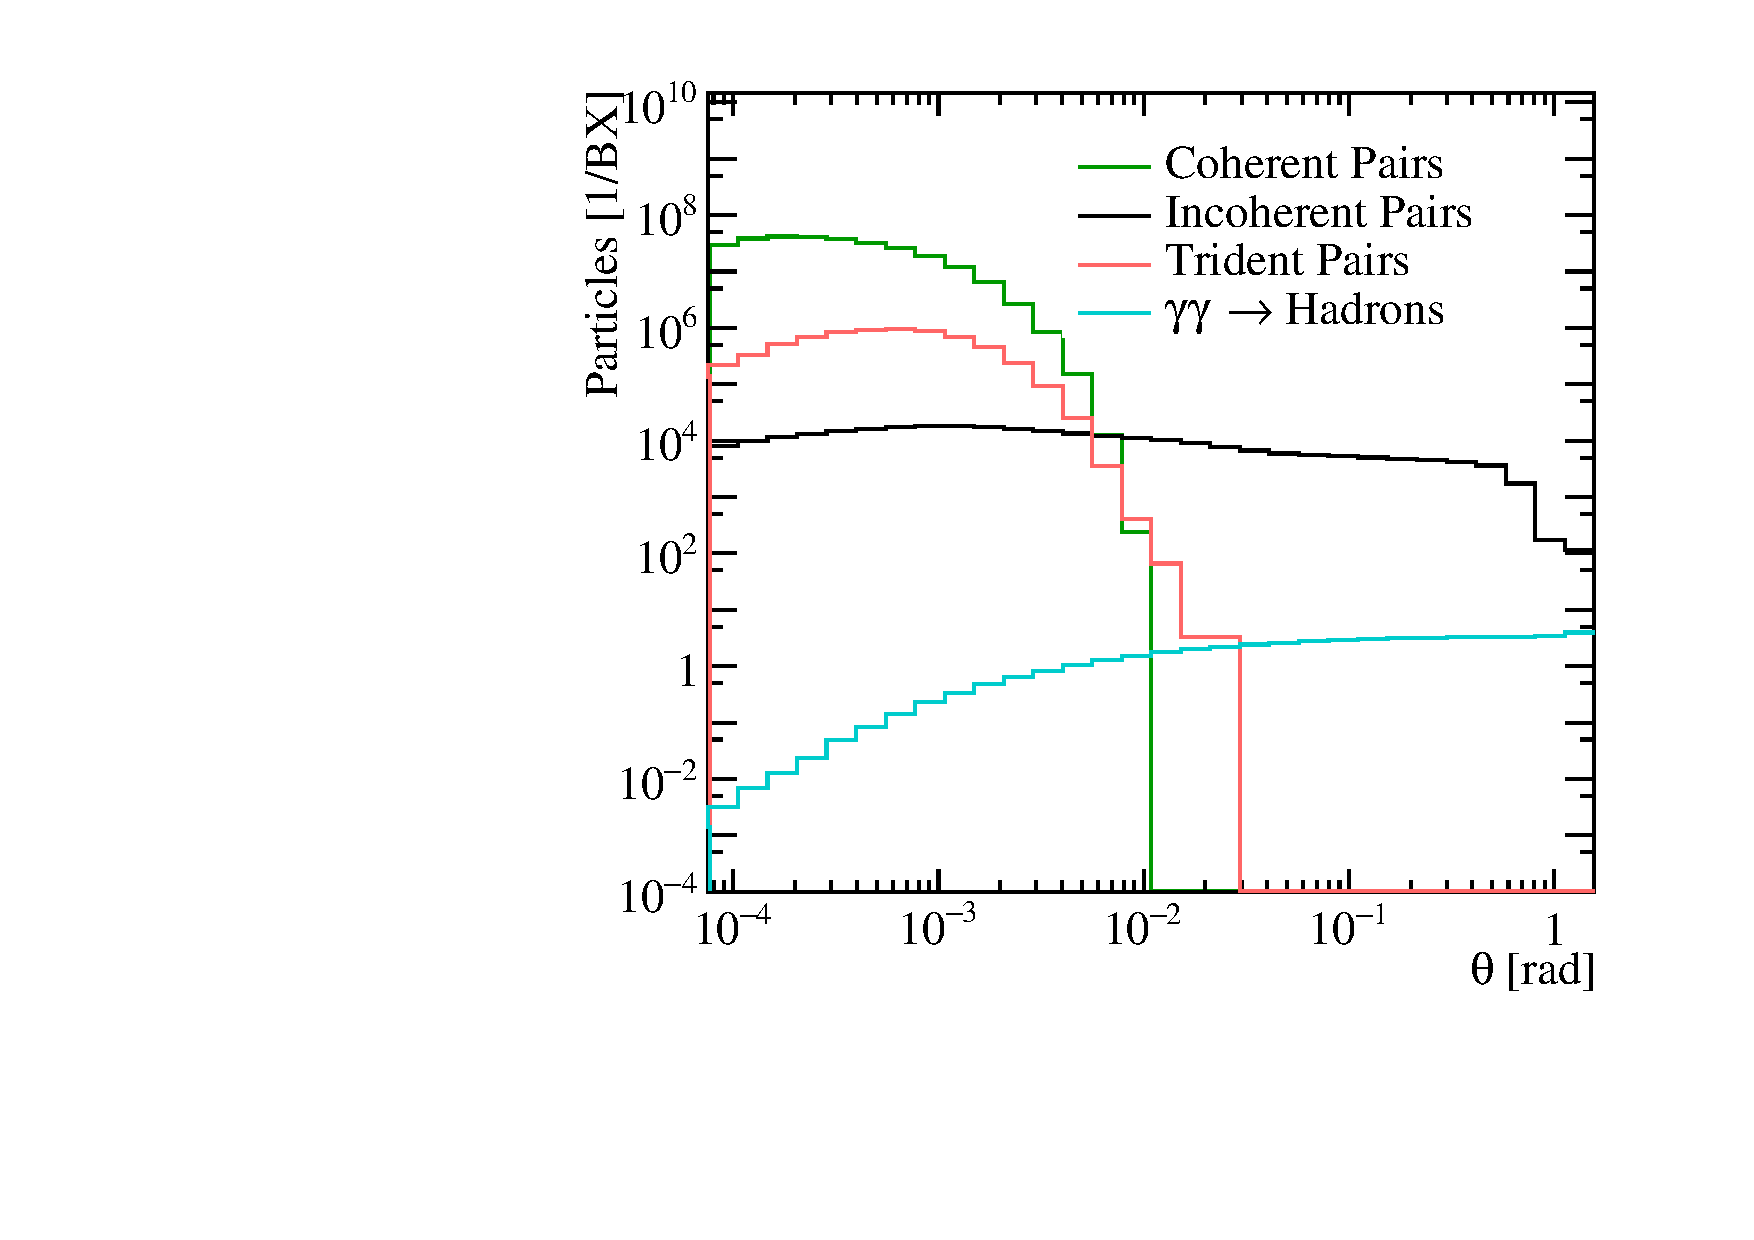
\includegraphics[width=0.5\textwidth]{PhysicsAnalysis/Plots/CDRPlots/BackgroundAngleCut.pdf}
\caption[]{Angular distribution of number of particles for beam induced backgrounds for CLIC at $\sqrt{s} = 3$ TeV.  Taken from CLIC CDR.}
\label{fig:backgroundangle}
\end{figure}

\section{Analysis}
The focus of this section is to describe the post reconstruction procedure applied to the signal and background events, described in \ref{sec:crosssectioncheck}, to extract the relevant information needed for this sensitivity study. 

\subsection{Jet Pairing} 
\label{sec:jetpairing}
The MarlinFastJet processor, a wrapper for the FastJet \cite{Cacciari:2011ma} processor, is used to cluster the signal and background events into four jets.  In the case of the signal final state, $\nu\nu$qqqq, it is assumed these four jets have arisen from the hadronic decays of the bosons involved in the vector scattering process.  These jets are paired up on the assumption that the correct pairing is achieved when the invariant masses of the two pairs are closest together. 

The longitudinally invariant $k_{t}$ jet algorithm in exclusive mode was used for the jet clustering.  In contrast to the inclusive mode, the exclusive mode allows the user to request a fixed number of jets in the output from MarlinFastJet.  The longitudinally invariant $k_{t}$ algorithm proceeds as follows:
\begin{itemize}
\item For each pair of particles, i and j, the $k_{t}$ distance, $d_{ij}$, and beam distance, $d_{iB} = p_{t}^{2}$, are calculated.
\begin{equation}
d_{ij} = \text{min}(p_{ti}^{2}, p_{tj}^{2}){\Delta}R^{2}_{ij}/R^{2}
\end{equation}
where ${\Delta}R^{2}_{ij} = (y_{i} - y_{j})^2 + (\phi_{i} - \phi_{j})^2$, $p_{t}$ is the transverse momentum of the particle with respect to the beam axis, $y_{i}$ is the rapidity of particle i and $\phi_{i}$ is the azimuthal angle of particle i. $R$ is a configurable parameter that typically is of the order of 1.
\item The minimum distance, $d_\text{min}$, of all the $k_{t}$ and beam distances is found.  If the minimum occurs for a $k_{t}$ distance, merge particles i and j, summing their 4-momenta in the energy combination scheme.  If the beam distance is the minimum, declare particle i to be apart of the "beam" jet.  Remove this particle from the list of particles and do not included in the final jet output.
\item Repeat until the requested number of jets have been created, or inclusive mode no particles are left in the event.
\end{itemize}

Two other clustering algorithms were considered, but, as figure \ref{fig:eventweights1400raw} shows, were found to be inappropriate for the experimental conditions at CLIC.  These alternative algorithm choices are applied in the same manor as the longitudinally invariant $k_{t}$ algorithm, however, they differ in their for the $k_{t}$ distance, $d_{ij}$, and beam distance, $d_{iB}$.

The first alternative jet algorithm considered was the $k_{t}$ algorithm for $\text{e}^{+}\text{e}^{-}$ colliders (or Durham algorithm) where $d_{ij} = 2\text{min}(E_{i}^{2}, E_{j}^{2})(1-cos\theta_{ij})$ and $d_{iB}$ is not used.  $\theta_{ij}$ is the opening angle of particles i and j meaning that in the collinear limit $d_{ij}$ corresponds to the relative transverse momenta of the particles.  The major failure of this algorithm when applied to CLIC is the absence of $d_{iB}$, which leads to many beam related background particles being associated to jets.  As figure \ref{fig:eventweights1400raw} shows, the invariant mass of the paired jets, which is expected to be centred around the W and Z boson masses, is much larger than expected, due to the presence of the beam related backgrounds in the jets.  Also this algorithm is not invariant to boosts along the beam direction making it inappropriate to use at CLIC as the beam induced backgrounds modify the nominal collision kinematics.  

The second alternative jet algortihm considered was the Cambridge/Aachen jet algorithm where $d_{ij} = {\Delta}R_{ij}^{2}/R^2$ and $d_{iB} = 1$.  This algorithm gave poor performance as does not account for the transverse momentum or energy of the particles being clustered. In essence, this is a cone clustering algorithm with a cone radius defined through ${\Delta}R_{ij} = R$, which even for large R was found to discard too much energy in the event to be useful for this analysis.  This can be seen in figure \ref{fig:eventweights1400raw} as the invariant mass of the paired jets is much lower than expected.  This algorithm is useful for events with highly boosted jets, but at CLIC the jets are too disperse.

\begin{figure}
\centering
\subfloat[]{\label{fig:invariantmassalgoveto1400GeV}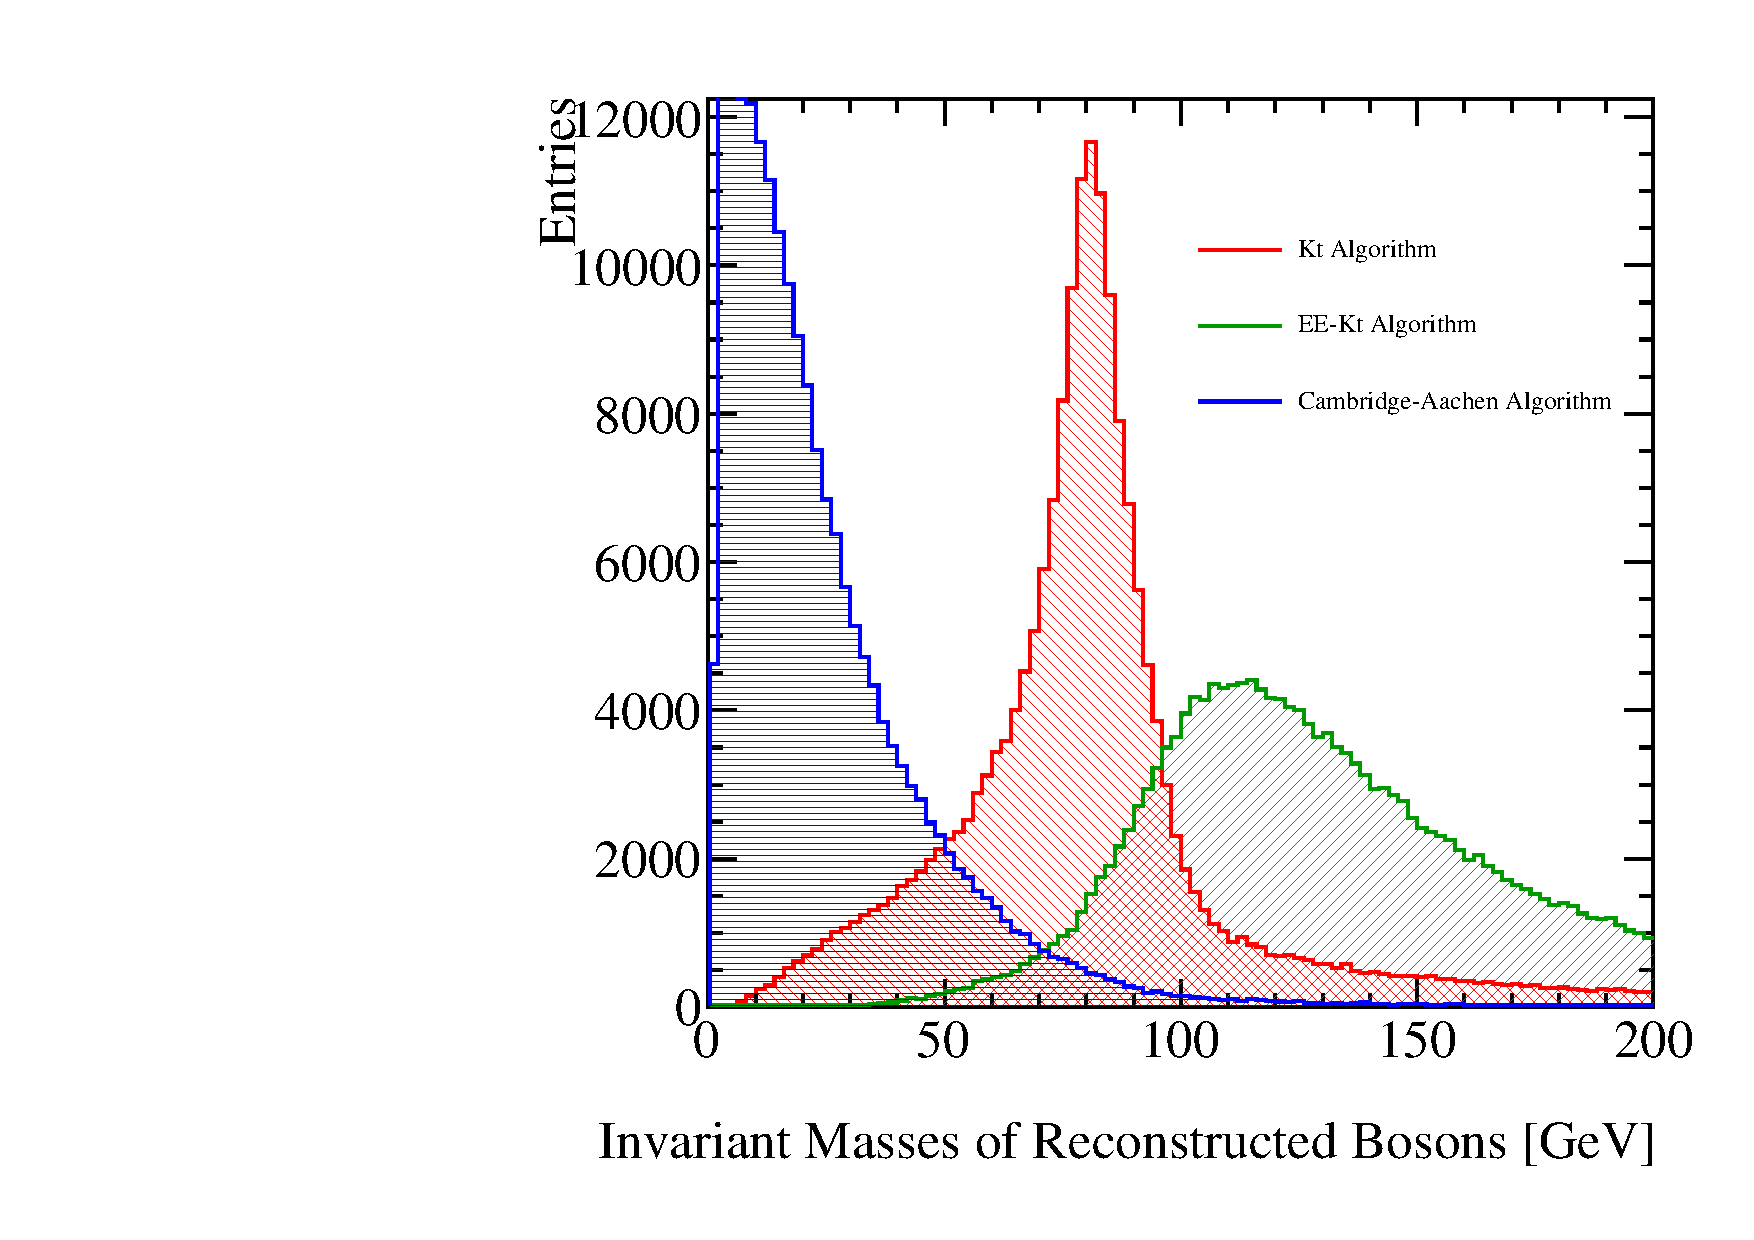
\includegraphics[width=0.5\textwidth]{PhysicsAnalysis/Plots/SimpleInvMassPlot/InvariantMassesAlgorithmVeto.pdf}}
\subfloat[]{\label{fig:invariantmassalgoveto3000GeV}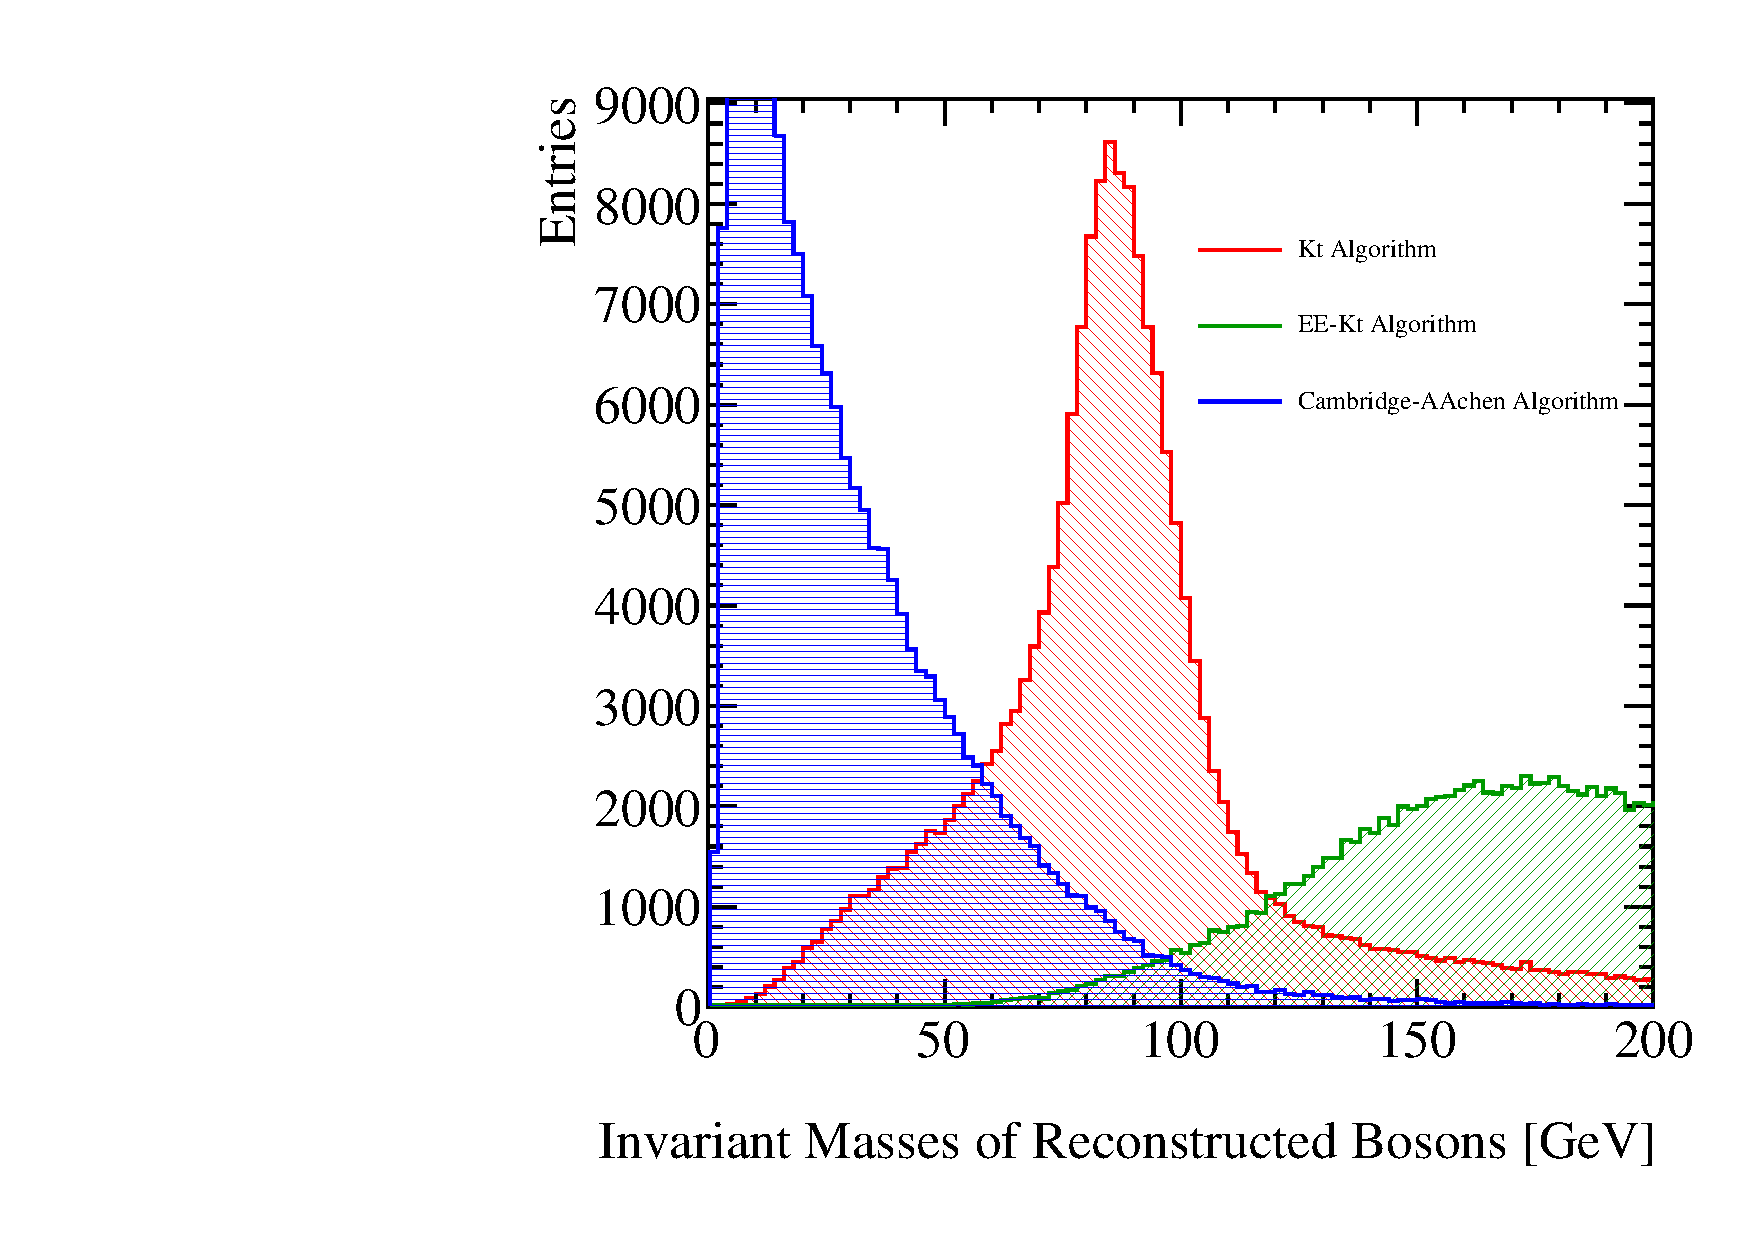
\includegraphics[width=0.5\textwidth]{PhysicsAnalysis/Plots/SimpleInvMassPlot/InvariantMassesAlgorithmVeto3000GeV.pdf}}
\caption[Reconstructed invariant masses for different choices of jet algorithm for 1.4 TeV and 3 TeV \nu{\nu}qqqq events.]{Reconstructed masses for different choices of jet algorithm for 1.4 TeV and 3 TeV \nu{\nu}qqqq events. These masses arise by forcing the reconstructed events into 4 jets and then pairing up the jets into pairs such that the reconstructed invariant masses of the pairs are closest to each other. These samples should be dominated by vector boson scattering involving pairs of W bosons and so it is expected that a peak at the W boson true mass should be observed. As this does not occur for the Cambridge-Aachen algorithm or the ee\_kt algorithm they were deemed unsuitable for this analysis at both 1.4 and 3 TeV. In the case of the kt algorithm and the ee\_kt algorithm an R parameter of 0.7 was used.}
\label{fig:eventweights1400raw}
\end{figure}

\subsection{Isolated Lepton Finding} 
\label{sec:isolatedleptonfinding}

\textcolor{red}{Unsure of details needed in this section.}

An isolated lepton finder is included in the analysis chain in an attempt to reject background events containing leptons. 

\subsection{Flavour Tagging} 
\label{sec:flavourtagging}

\textcolor{red}{Don't actually use in this analysis.  I assume I skip this section.}
The LCFIPlus \cite{Suehara:2015ura} processor is also run on these events once clustered into jets to produce a value for the B and C tag likelihood for a jet.  

This information is available for background rejection rather than contributing to the sensitivity of the event to the anomalous couplings. The LCFIPlus vertex processor was trained using events of $\text{e}^{+}\text{e}^{-}\rightarrow \text{Z}\nu\nu \rightarrow \text{q}\bar{\text{q}}\nu\nu$ for q = u,d,s,c,b.

\subsection{Analysis Processor} 
\label{sec:analysisprocessor}
\textcolor{red}{Best way to show this?}

Finally, an analysis processor is run, which calculates a number of variables used downstream in the analysis. Included in these are:
\begin{itemize}
\item Number of PFOs in the jets and the paired up bosons.
\item Number of charged PFOs in the jets and paired up bosons.
\item Highest energy PFO: energy, momentum, transverse momentum, $cos\theta$.
\item Highest energy electron PFO: energy, momentum, transverse momentum, $cos\theta$.
\item Highest energy muon PFO: energy, momentum, transverse momentum, $cos\theta$.
\item Highest energy photon PFO: energy, momentum, transverse momentum, $cos\theta$.
\item (If in existence) Highest and second highest energy isolated lepton: energy, momentum, transverse momentum, $cos\theta$.
\item Bosons: energy, momentum, transverse momentum, $cos\theta$.
\item Invariant mass of the boson pair.
\item Jets: energy, momentum, transverse momentum, $cos\theta$.
\item $Cos\theta$ Of the missing 3-momentum vector.
\item Recoil mass.
\item Invariant mass of the visible system.
\item $y_{i}$, $y_{i+1}$. Jet clustering parameters ranging from i = 0 to 6.
\item $Cos\theta^{*}_{Jet}$.  This is the opening angle of a pair of jets, assumed to be from a signle boson, in the rest frame of the boson.
\item $Cos\theta^{*}_{Boson}$.  This is the opening angle of a pair of bosons, assumed to be from vector boson scattering, in the rest frame of the di-boson pair.
\item Transverse momentum and energy of the event.
\item Acolinearity of the jet pairs forming the bosons and the acoilinearity of the boson pair.
\item Principle thrust $T$ and the thrust axes $\bar{\textbf{n}}$. Note $\bar{\textbf{n}}$ is a unit vector. These are defined by the following equation
\begin{equation}
T = \text{max}_{\bar{\textbf{n}}} (\frac{\Sigma_{i} \textbf{p}_{i}.\bar{\textbf{n}}}{\Sigma_{i} |\textbf{p}_{i}|^{2}})
\end{equation}
\item The major and minor thrust values. These are defined with respect to the thrust axes $\bar{\textbf{n}}$ in the following way:
\begin{equation}
T = \text{max}_{\bar{\textbf{n}}_{major}} (\frac{\Sigma_{i} \textbf{p}_{i}.\bar{\textbf{n}}_{major}}{\Sigma_{i} |\textbf{p}_{i}|^{2}})
\end{equation}
where $\bar{\textbf{n}}_{major}.\bar{\textbf{n}} = \textbf{0}$. Similarly the minor thrust value is defined as 
\begin{equation}
T = \frac{\Sigma_{i} \textbf{p}_{i}.\bar{\textbf{n}}_{minor}}{\Sigma_{i} |\textbf{p}_{i}|^{2}}
\end{equation}
where $\bar{\textbf{n}}_{minor}.\bar{\textbf{n}} = \bar{\textbf{n}}_{minor}.\bar{\textbf{n}}_{major} =\textbf{0}$
\item Sphericity. This is defined using the sphericity tensor $S^{ab}$ defined as:
\begin{equation}
S^{ab} = \frac{\Sigma_{i}p^{\alpha}_{i}p^{\alpha}_{j}}{\Sigma_{i,\alpha=1,2,3}|p^{\alpha}_{i|^{2}}}
\end{equation}
Where $p_{i}$ are the components of the momenta of particle i in the frame of the detector and the sum runs over all particles in the event. Sphericity is defined as $\text{S} = \frac{3}{2}(\lambda_{2} + \lambda_{3})$, where $\lambda_{i}$ are the eigenvalues of the sphericity tensor defined such $\lambda_{1} \geq \lambda_{2} \geq \lambda_{3}$.  This provides a measure of how spherical the reconstructed event topology is with isotropic events having $S \approx 1$, while two jet events have $S \approx 0$.  (Also $\lambda_{1} + \lambda_{2} + \lambda_{3} = 1$.)
\item Aplanarity. Aplanarity is defined as $\frac{3}{2} \lambda_{3}$ where $\lambda_{3}$ is an eigenvalue of the sphericity tensor.  This provides a measure of whether an event is linear or planar.
\item B and C tag values for the jets, the min and max B and C tag values for the bosons.
\end{itemize}

Alongside these variables, for the \nu{\nu}qqqq final state a number of Monte-Carlo variables are calculated for informative purposes and are not used in the analysis. These include:
\begin{itemize}
\item The quark and neutrino 4 momenta.
\item Invariant mass of boson pair using MC pairing and MC energy.
\item Invariant mass of boson pair using MC pairing and reconstructed jet energy.
\end{itemize}

\section{Methodology for Fitting}
It is necessary to discuss the fitting procedure in this analysis as the optimisation of the jet algorithms relies on this methodology. In this section only the signal events are considered to determine the underlying sensitivity of the CLIC detector to the anomalous couplings. This decision was made to save analysis of the large number of background samples in the optimisation of the jet reconstruction algorithms, while still optimising the algorithm on the physics of interest.

\subsection{Choice of Fitting Distribution}
The sensitivity of CLIC to the anomalous gauge couplings is determined through the use of a $\chi^{2}$ fit to the distribution of $\text{cos}\theta^{*}_{Jets}$ where $\theta^{*}_{Jets}$ is the angle between the two jets produced from the hadronic decay of the W/Z boson in the rest frame of that boson.  The distribution of $\text{cos}\theta^{*}_{Jets}$ proved to be sensitive to the anomalous gauge couplings as shown in figure \ref{fig:costhetastarjets}.

Another distribution considered for the sensitivity study was  $\text{cos}\theta^{*}_{Bosons}$ where $\theta^{*}_{Bosons}$ is the angle between the two bosons produced in vector boson scattering in the rest frame of the boson pair.  This distribution was found to be less sensitive to the anomalous gauge couplings than $\text{cos}\theta^{*}_{Jets}$, which can be seen when comparing figures \ref{fig:costhetastarjets} and \ref{fig:costhetastarbosons}, and so was not considered for the rest of this study.  Furthermore, it was found that a two dimensional $\chi^{2}$ fit produced by combining $\text{cos}\theta^{*}_{Jets}$ and $\text{cos}\theta^{*}_{Bosons}$ did not improve the sensitivity significantly in comparison to $\text{cos}\theta^{*}_{Jets}$.

The $\text{cos}\theta^{*}_{Jets}$ variable was binned in histograms of 10 bins before begin converted into a value of $\chi^{2}$.  This binning was selected to maximise the number of bins in the distribution, while minimising the effect of large bin by bin fluctuations arising from individual events with large event weights.

\begin{figure}
\subfloat[1.4 TeV Events]{\label{fig:costhetastarjets1400GeV} 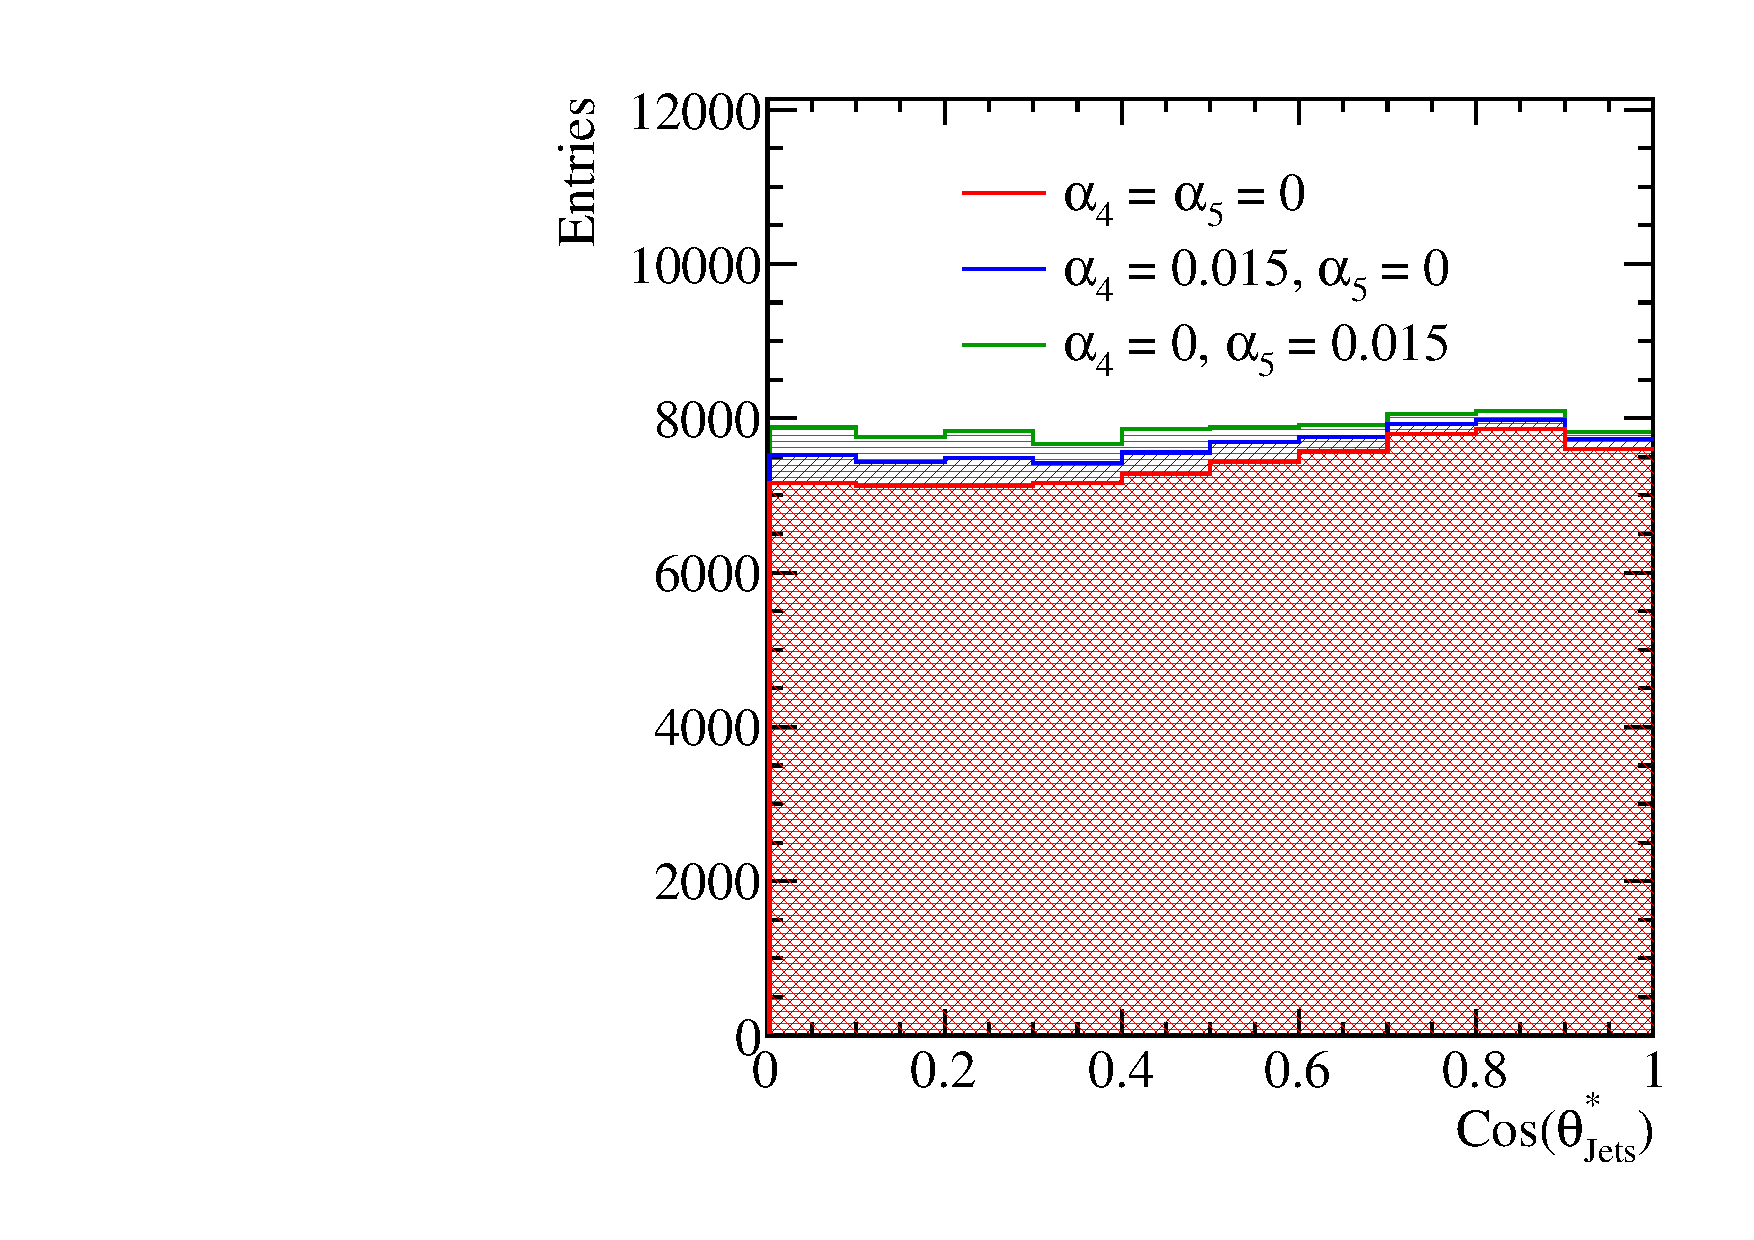
\includegraphics[width=0.5\textwidth]{PhysicsAnalysis/Plots/SensitiveDistributions/CosThetaStarSynJets_SPFOs_kt_0p70_1400GeV.pdf}}
\subfloat[3 TeV Events]{\label{fig:costhetastarjets3000GeV} 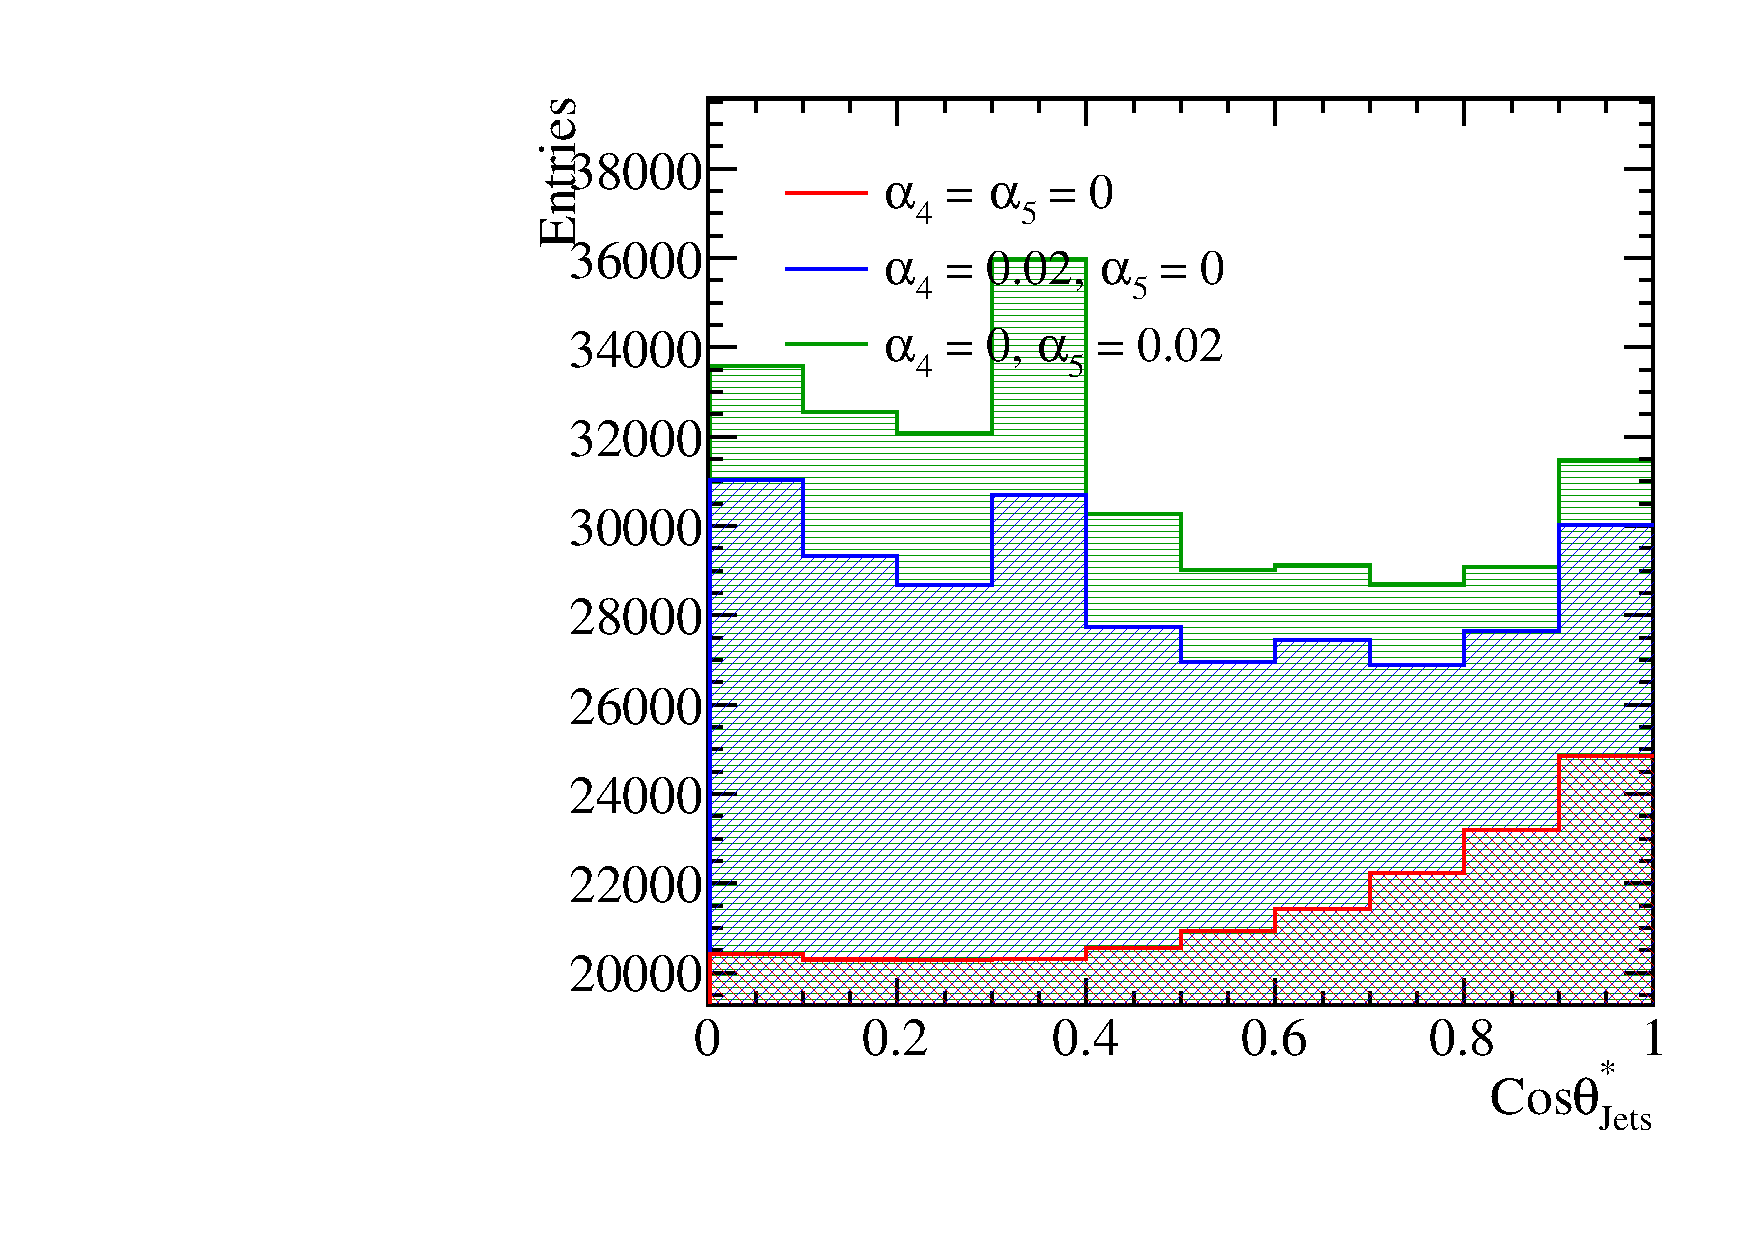
\includegraphics[width=0.5\textwidth]{PhysicsAnalysis/Plots/SensitiveDistributions/CosThetaStarSynJets_SPFOs_kt_0p70_3000GeV.pdf}}
\caption[Sensitivity of $\text{cos}\theta^{8}_{Jets}$ to the anomalous gauge couplings $\alpha_{4}$ and $\alpha_{5}$ at 1.4 and 3 TeV.]{Sensitivity of $\text{cos}\theta^{*}_{Jets}$ to anomalous couplings at 1.4 and 3 TeV. The jet algorithm used for this example was the longitudinally invariant kt algorithm with an R parameter of 0.7. This sample corresponds to pure signal of hadronic decays in vector boson scattering i.e. \nu{\nu}qqqq.}
\label{fig:costhetastarjets}
\end{figure}

\begin{figure}
\subfloat[1.4 TeV Events]{\label{fig:costhetastarbosons1400GeV} 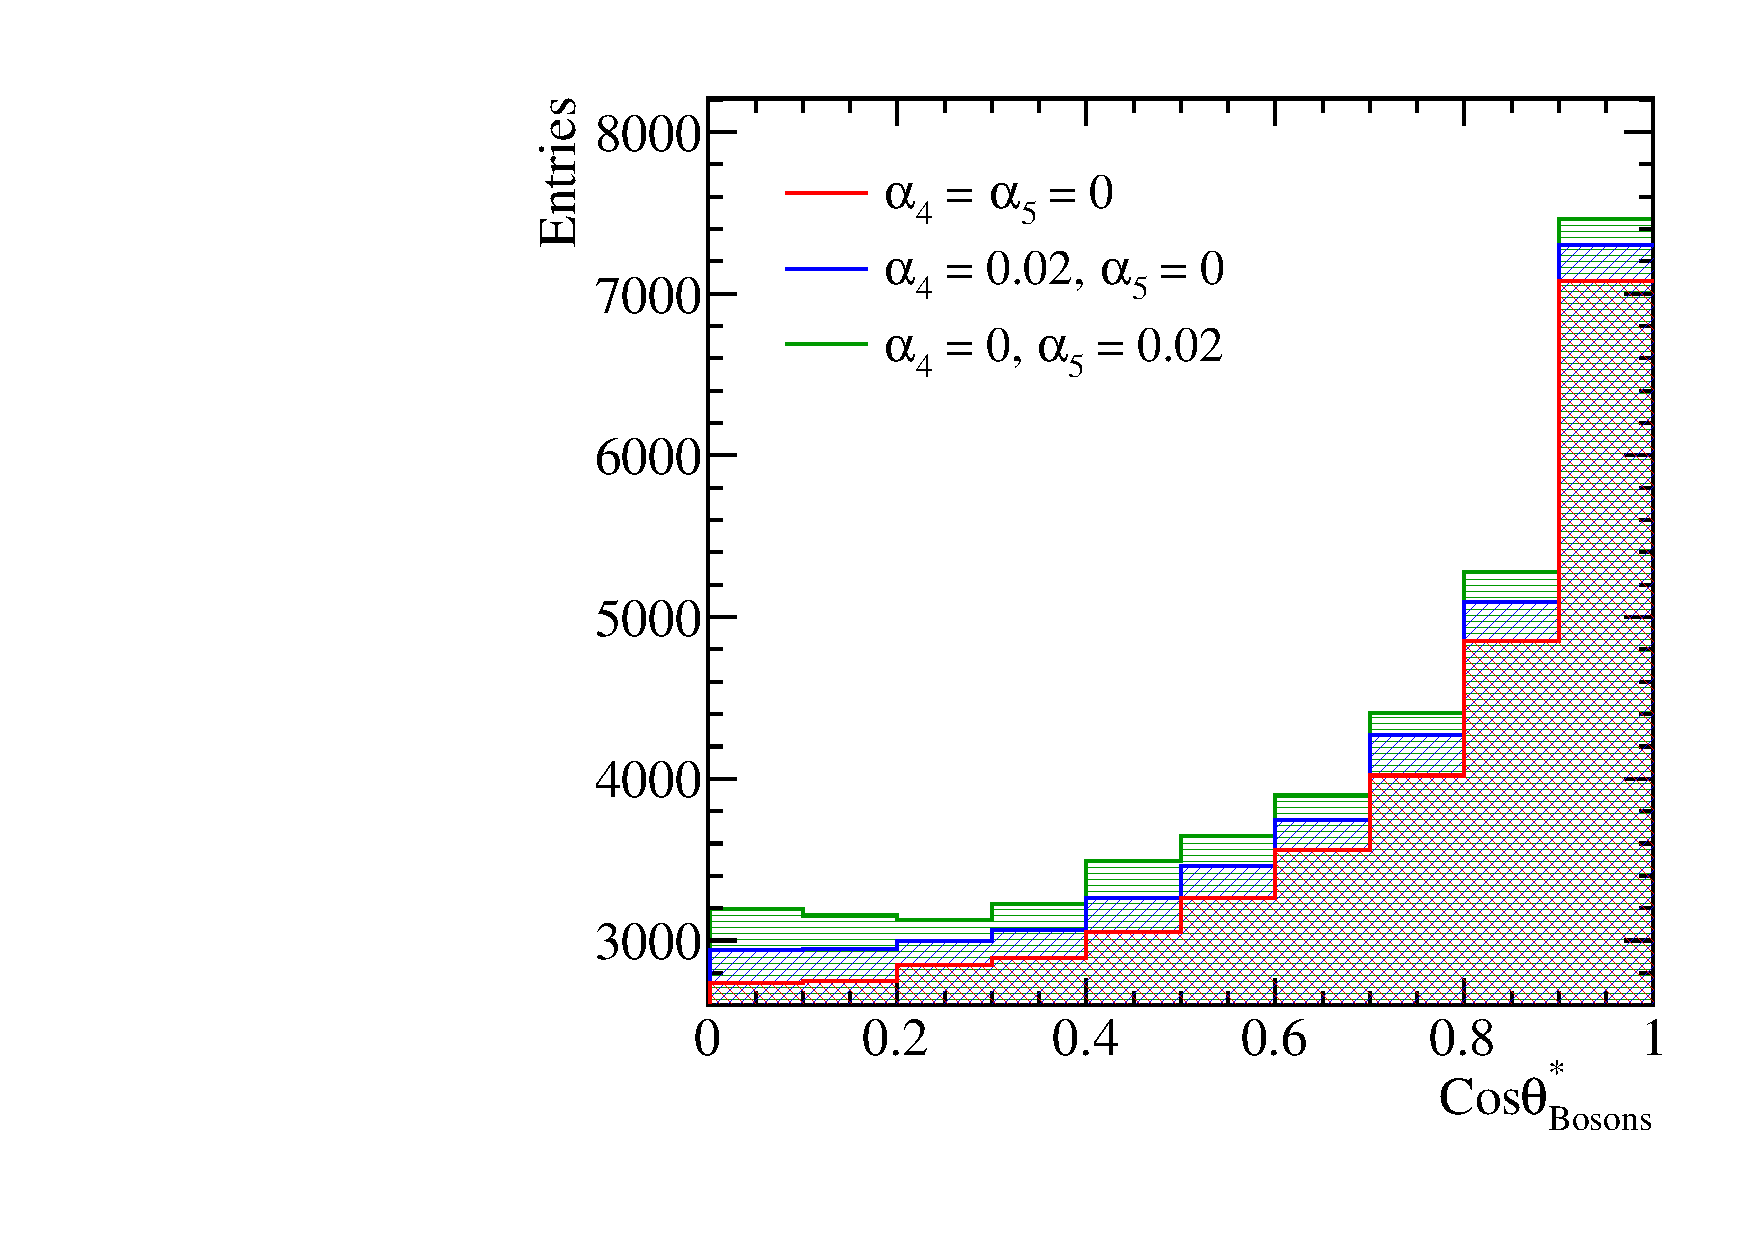
\includegraphics[width=0.5\textwidth]{PhysicsAnalysis/Plots/SensitiveDistributions/CosThetaStarSynBosons_SPFOs_kt_0p70_1400GeV.pdf}}
\subfloat[3 TeV Events]{\label{fig:costhetastarbosons3000GeV} 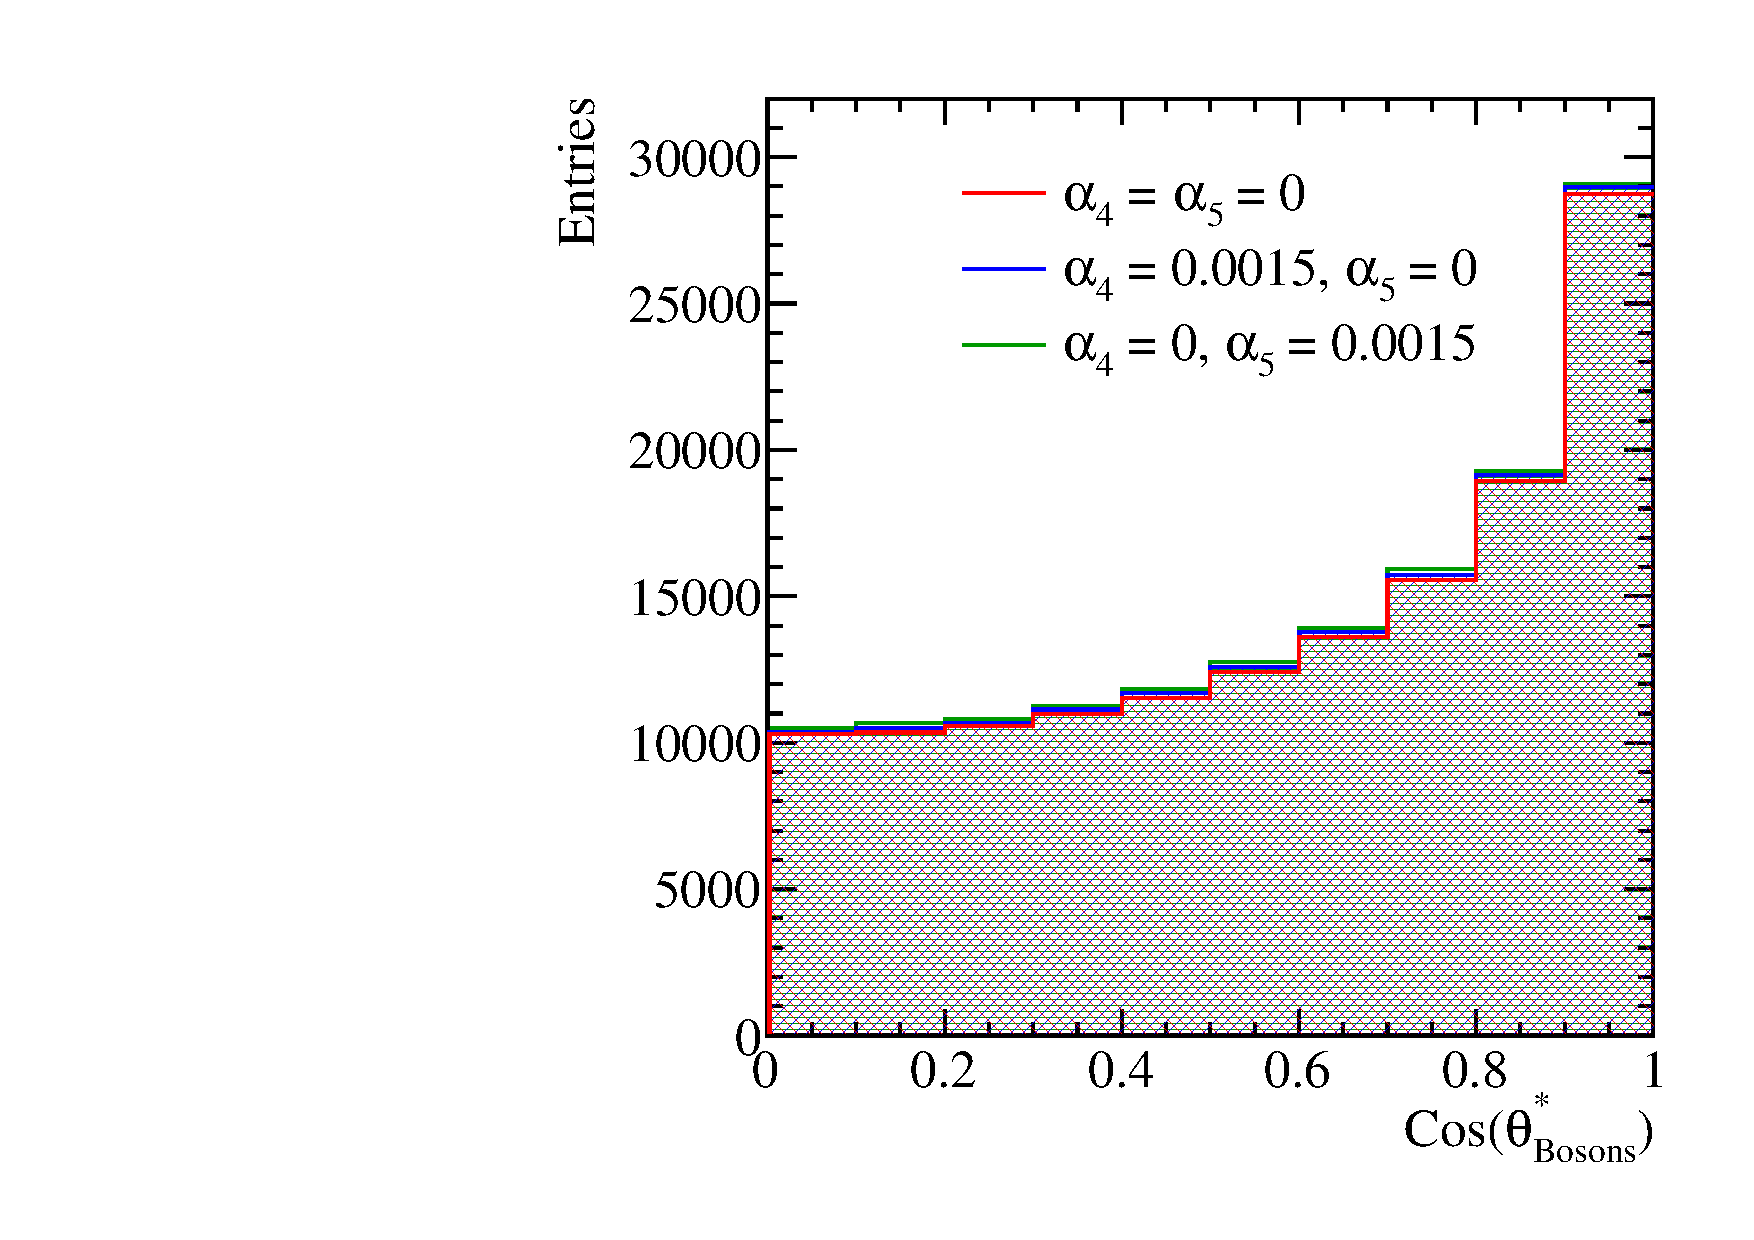
\includegraphics[width=0.5\textwidth]{PhysicsAnalysis/Plots/SensitiveDistributions/CosThetaStarSynBosons_SPFOs_kt_0p70_3000GeV.pdf}}
\caption[Sensitivity of $\text{cos}\theta^{8}_{Bosons}$ to the anomalous gauge couplings $\alpha_{4}$ and $\alpha_{5}$ at 1.4 and 3 TeV.]{Sensitivity of $\text{cos}\theta^{*}_{Bosons}$ to anomalous couplings at 1.4 and 3 TeV. The jet algorithm used for this example was the longitudinally invariant kt algorithm with an R parameter of 0.7. This sample corresponds to pure signal of hadronic decays in vector boson scattering i.e. \nu{\nu}qqqq.}
\label{fig:costhetastarbosons}
\end{figure}

\subsection{Event Weight Impact on Fitting Distribution}
At 1.4 TeV event weights were produced from Whizard stepping along $\alpha_{4}$ and $\alpha_{5}$ in steps of 0.01 ranging from -0.07 to 0.07 as shown in figure \ref{fig:eventweights1400raw}, however, to produce a smooth $\chi^{2}$ contour much finer sampling is needed.  While it is feasible to generate new event weights in Whizard for any pair of $\alpha_{4}$ and $\alpha_{5}$ it is time consuming making it impractical for this analysis.  To overcome this difficulty bicubic interpolation is applied between these points to allow for the extract of event weights anywhere within the range -0.05 to 0.05.  As figure \ref{fig:eventweights1400interpolated} shows the interpolated surface proves to be a good fit to the data produced from the generator in that it is smooth and continuous.  

Similarly at 3 TeV the same procedure was used but stepping occurs in steps of 0.001 ranging from -0.007 to 0.007 in both $\alpha_{4}$ and $\alpha_{5}$.  These ranges proved to be sufficient for the contours of interest for the CLIC sensitivity analysis at this energy.

\begin{figure}
\centering
\subfloat[]{\label{fig:weight1}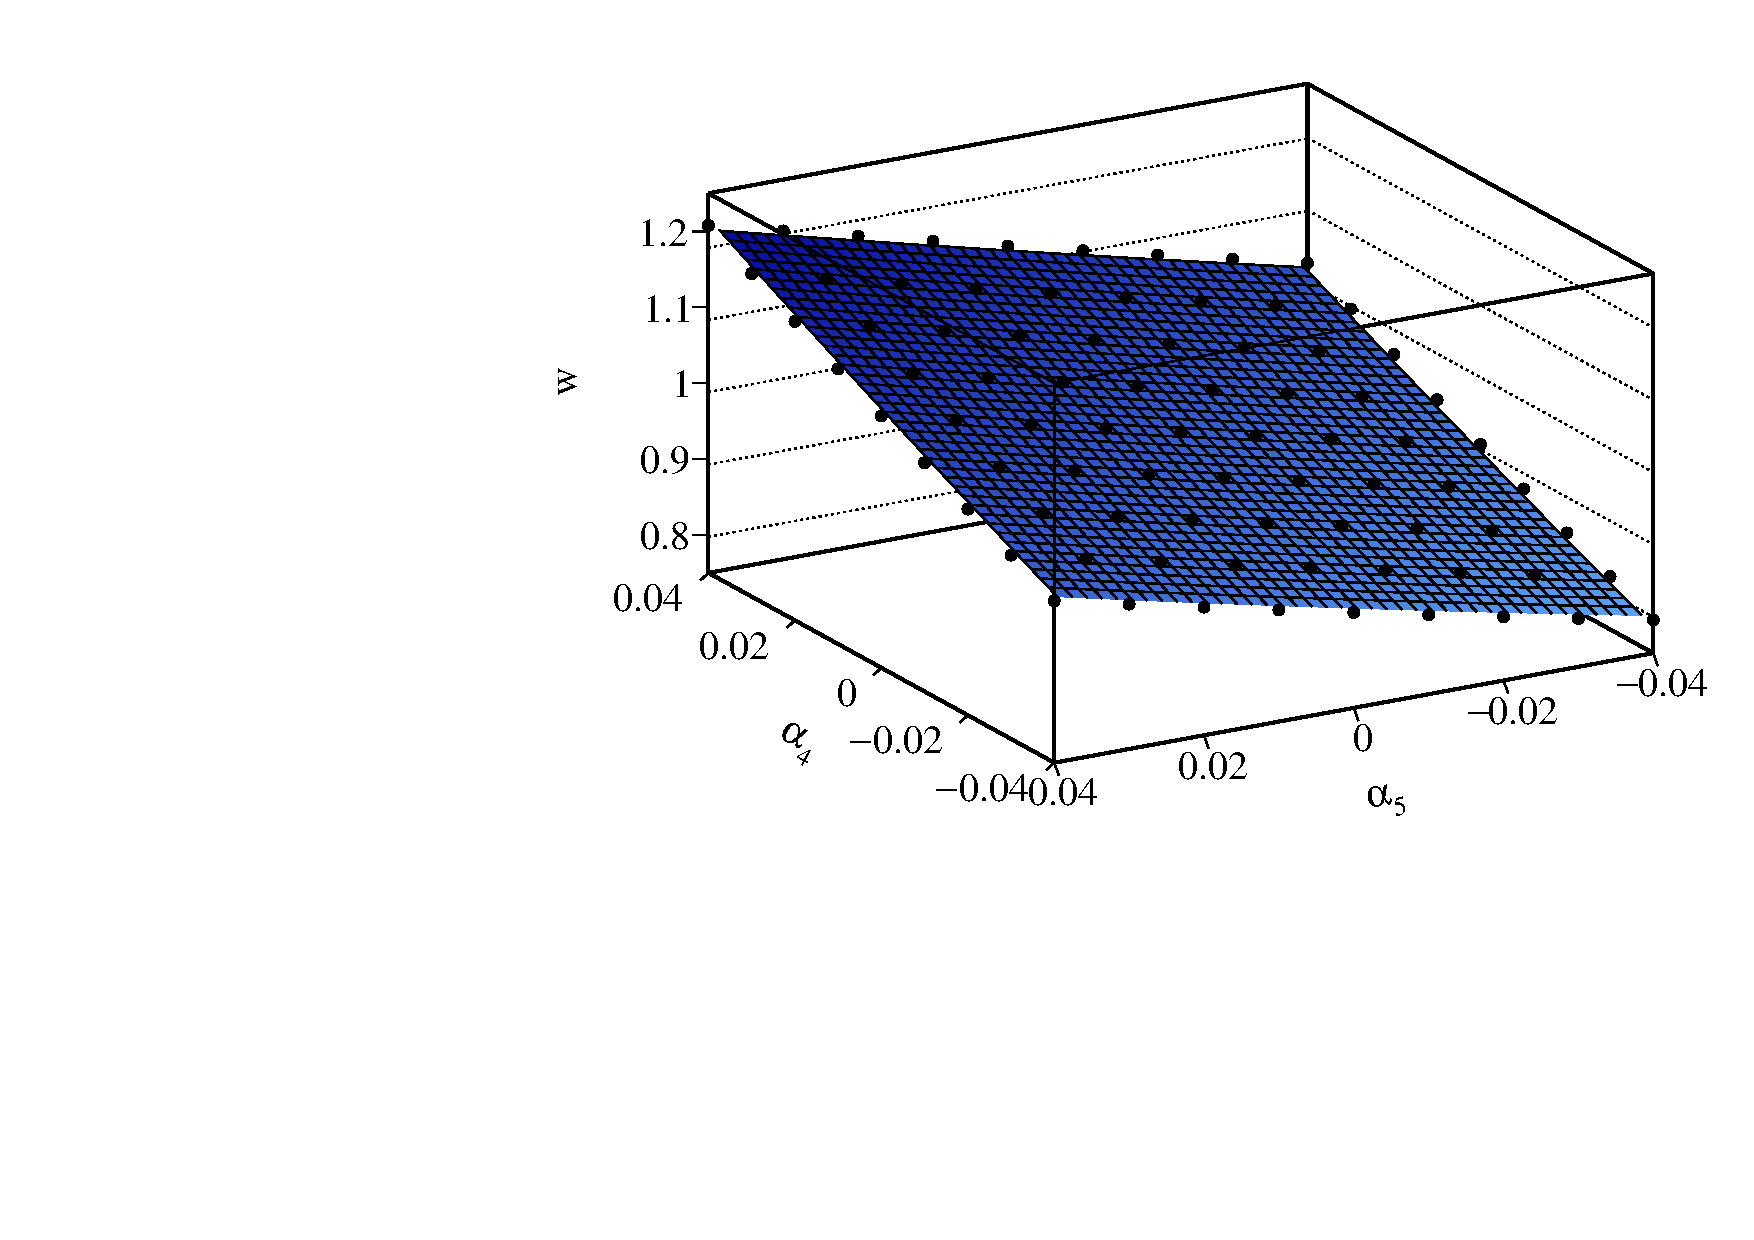
\includegraphics[width=0.5\textwidth]{PhysicsAnalysis/Plots/EventWeights/1400GeV/EventWeightsForEvent100001009_1400GeV_SPFOs_kt_0p70_10Bins_Start_0_End_10_1400GeV_Interpolated.pdf}}
\subfloat[]{\label{fig:weight2}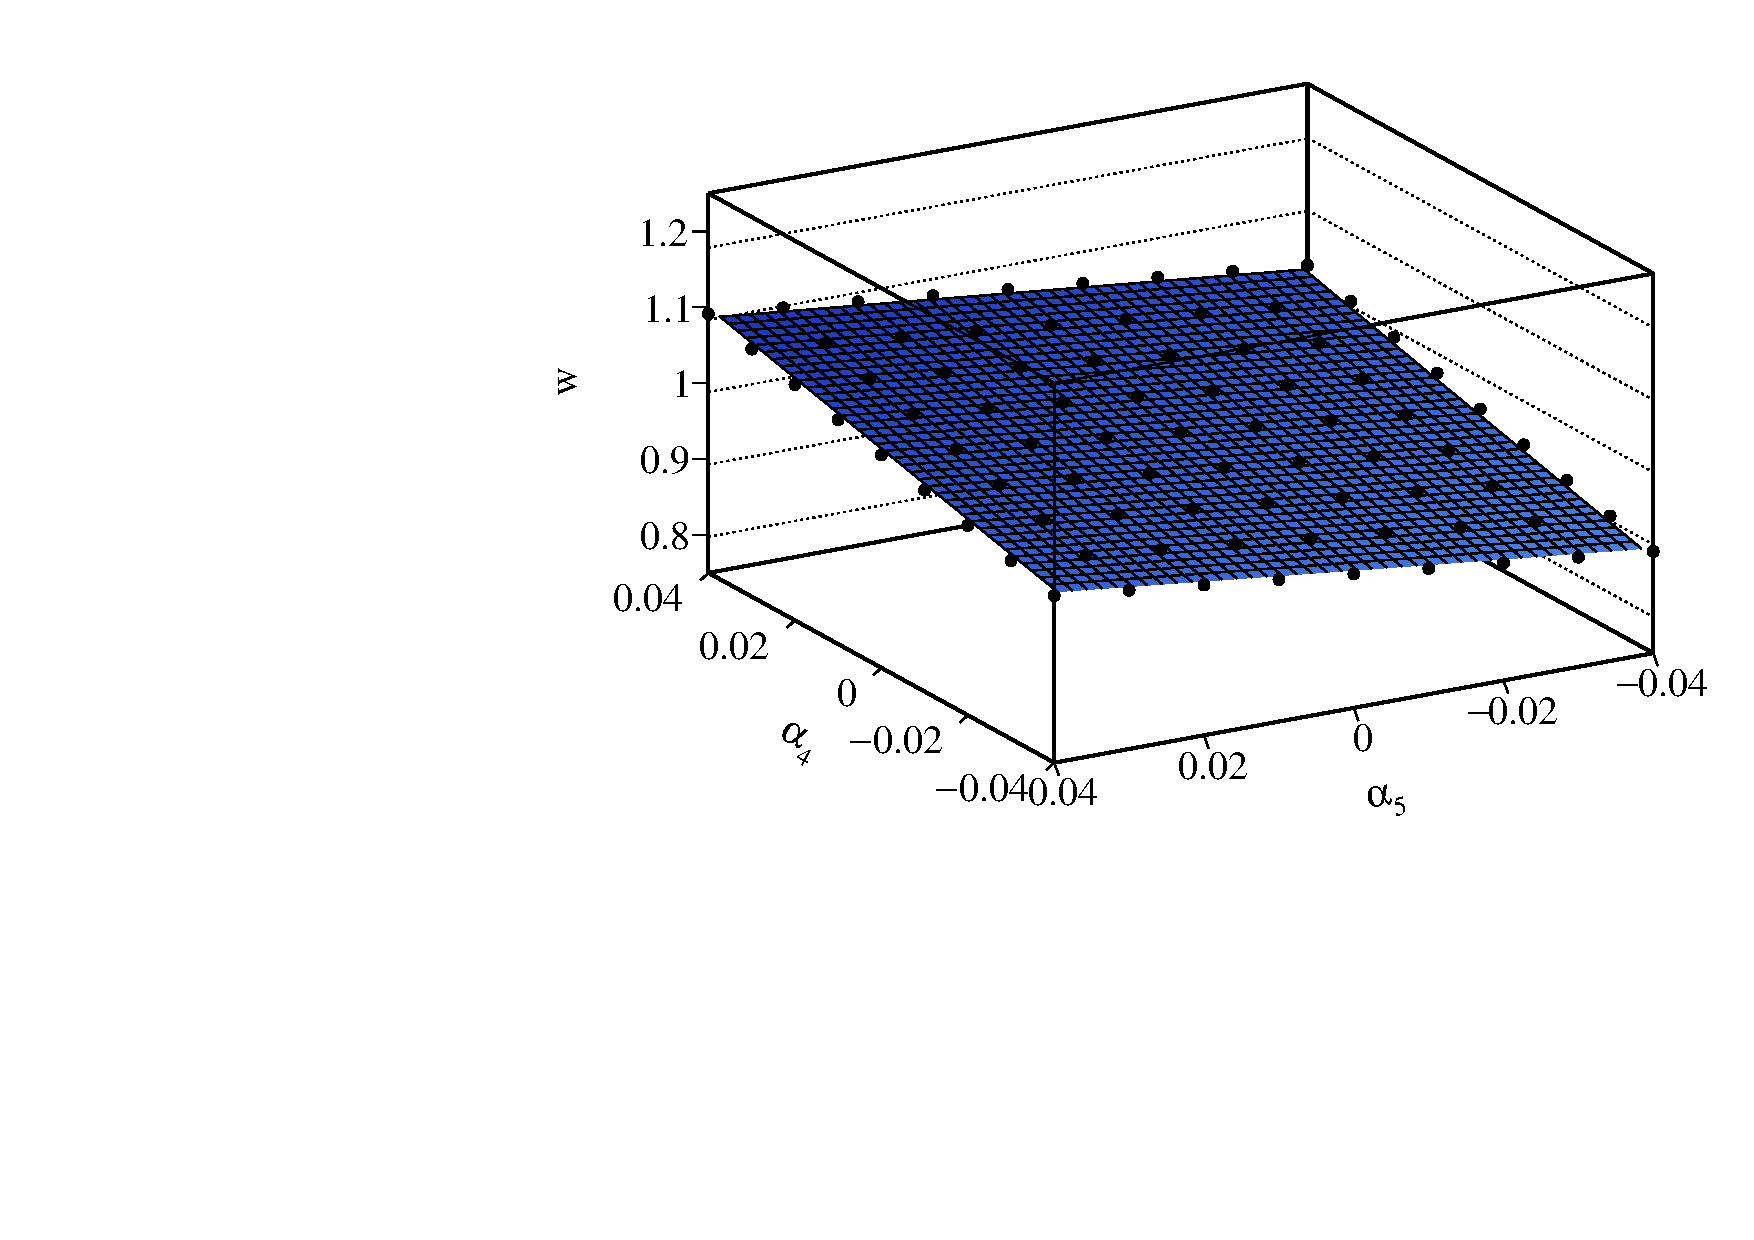
\includegraphics[width=0.5\textwidth]{PhysicsAnalysis/Plots/EventWeights/1400GeV/EventWeightsForEvent100001014_1400GeV_SPFOs_kt_0p70_10Bins_Start_0_End_10_1400GeV_Interpolated.pdf}} \hfill
\subfloat[]{\label{fig:weight3}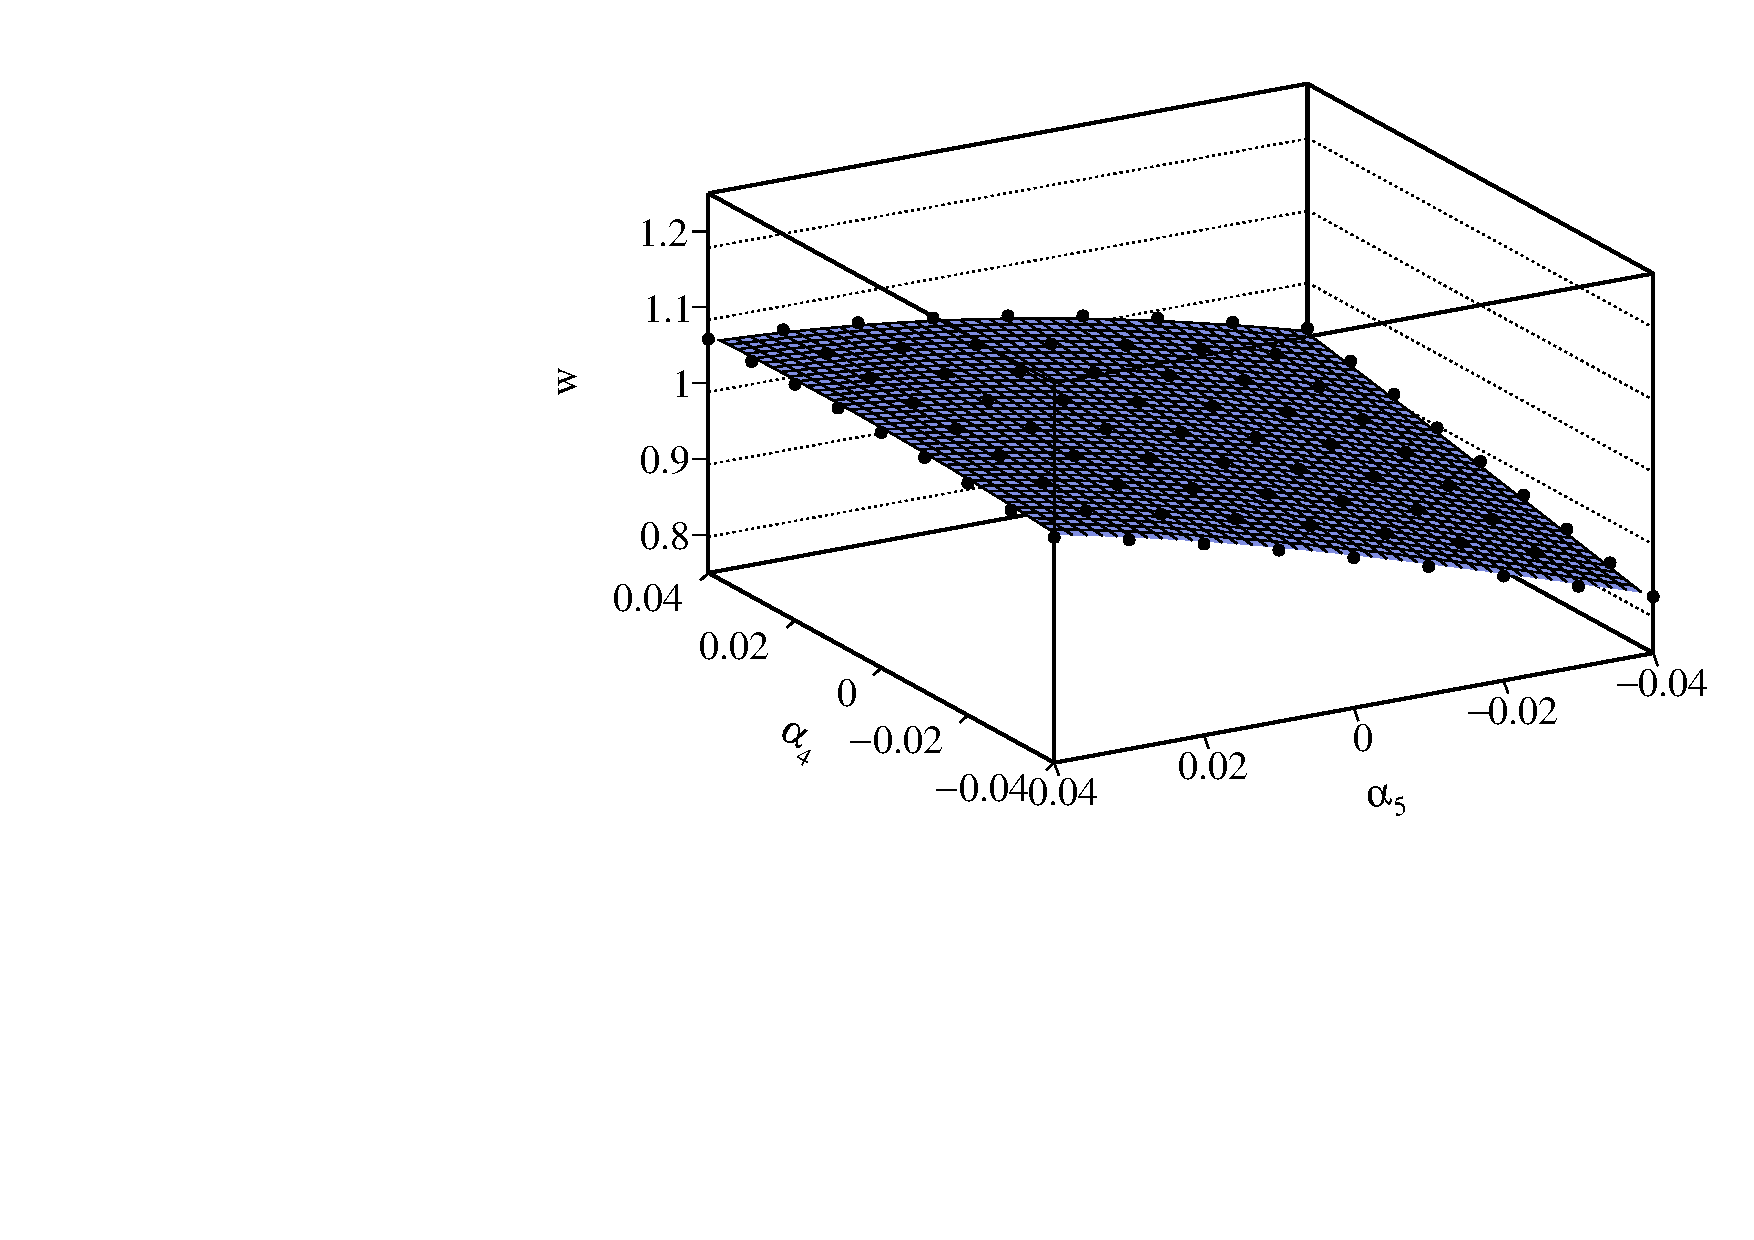
\includegraphics[width=0.5\textwidth]{PhysicsAnalysis/Plots/EventWeights/1400GeV/EventWeightsForEvent100001044_1400GeV_SPFOs_kt_0p70_10Bins_Start_0_End_10_1400GeV_Interpolated.pdf}}
\subfloat[]{\label{fig:weight4}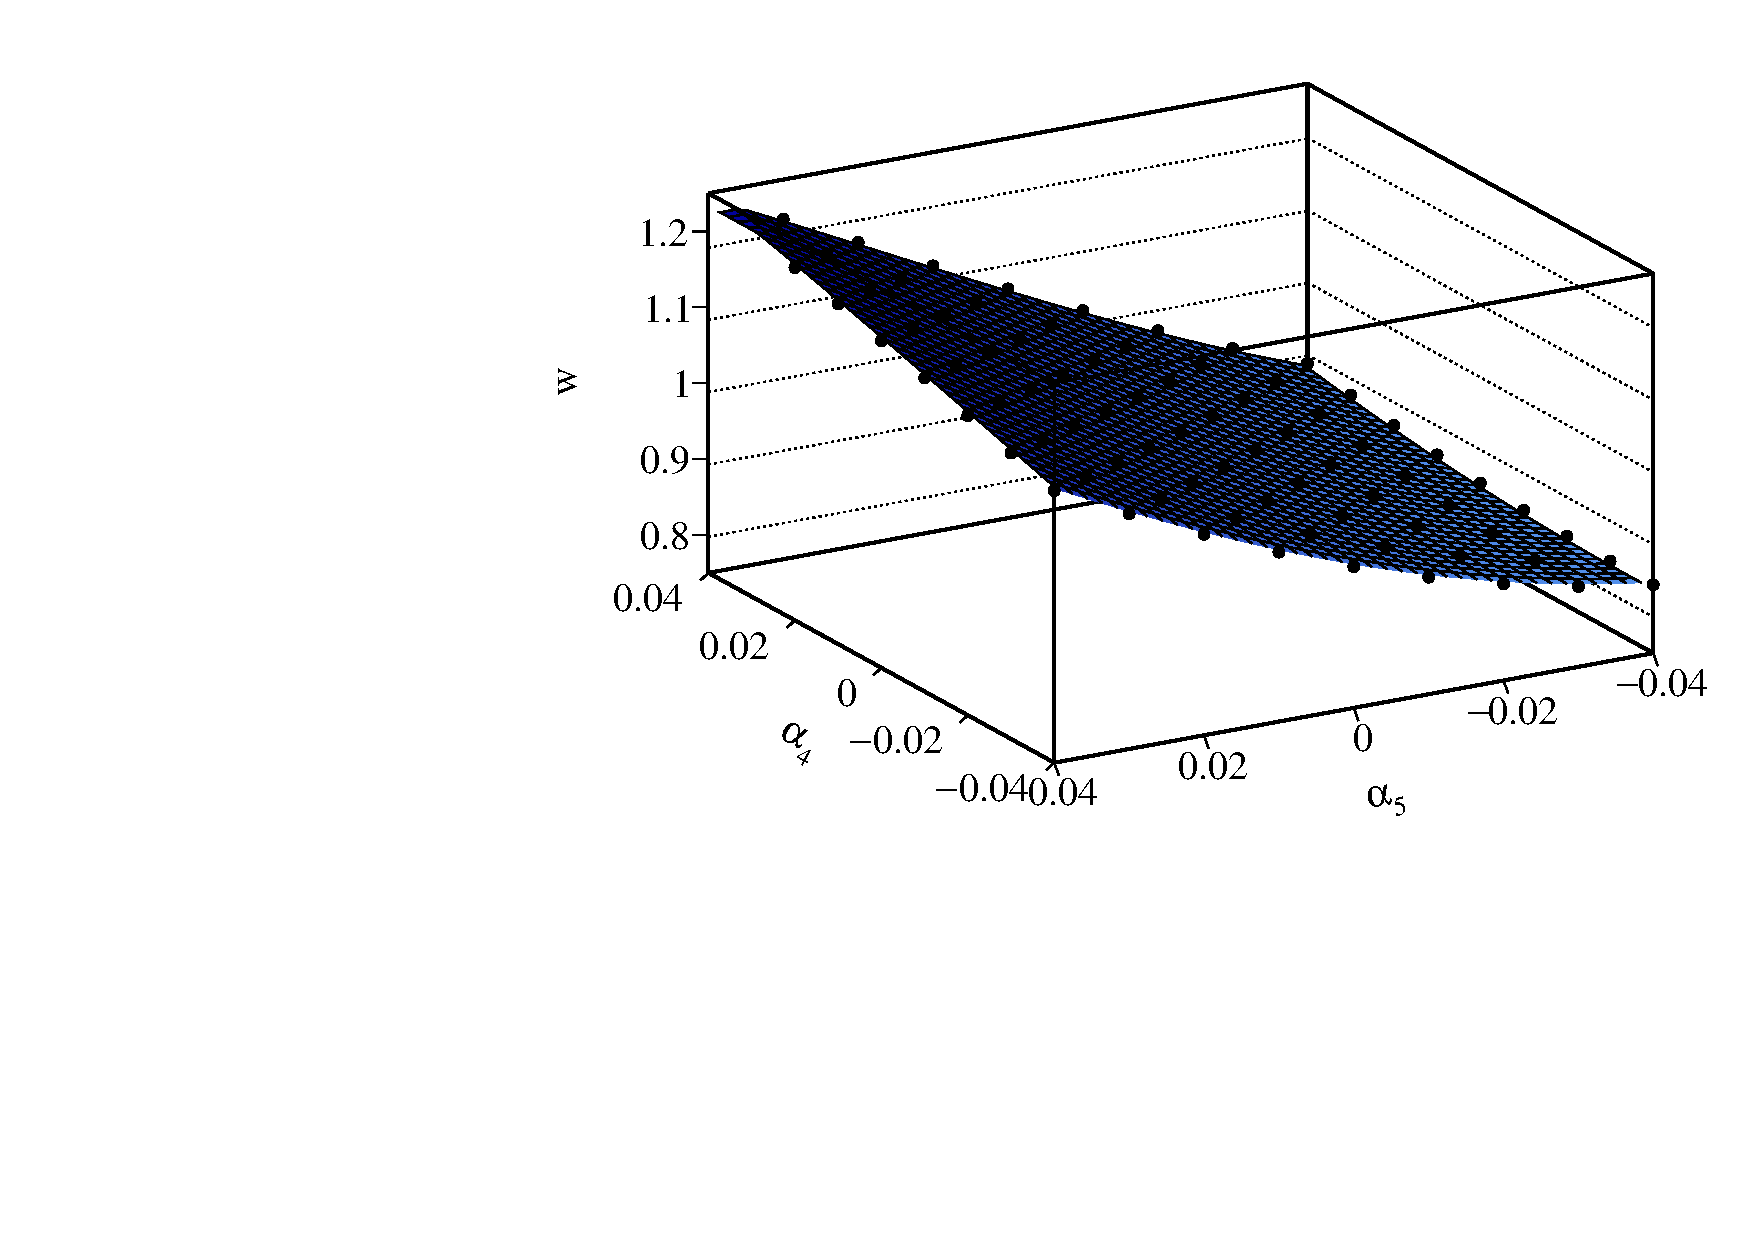
\includegraphics[width=0.5\textwidth]{PhysicsAnalysis/Plots/EventWeights/1400GeV/EventWeightsForEvent100001051_1400GeV_SPFOs_kt_0p70_10Bins_Start_0_End_10_1400GeV_Interpolated.pdf}}
\caption[Event weights from Whizard for 1.4TeV \nu{\nu}qqqq final state events with interpolated surface.]{A selection of plots showing how the event weight changes when varying the anomalous couplings $\alpha_{4}$ and $\alpha_{5}$ for 1.4TeV \nu{\nu}qqqq final state events.  The hollow circles show the event weight produced from the generator while the surface shown is found using bicubic interpolation between those points.}
\label{fig:eventweights1400interpolated}
\end{figure}

\subsection{Analysis of Fitting Distribution}
Using these interpolated surfaces for the event weights, distribution of $\text{cos}\theta^{*}_{Jets}$ were produced stepping across $\alpha_{4}$ and $\alpha_{5}$ in steps of 0.0001 at 1.4 TeV and 0.00001 at 3 TeV.  Each distribution was converted into a value of $\chi^{2}$ using the following formula:

\begin{equation}
\chi^{2} = \Sigma_{i} \frac{(O_{i} - E_{i})^{2}}{E_{i}}
\end{equation}

where $O_{i}$ is the observed bin content for bin i in the distribution with non-zero $\alpha_{4}$ and $\alpha_{5}$ and $E_{i}$ is the expected bin content for bin i in the distribution with zero $\alpha_{4}$ and $\alpha_{5}$ i.e. the standard model expected value.

Confidence limits indicate the probability of measuring a given value of $\chi^{2}$ in the $\alpha_{4}$ and $\alpha_{5}$ space.  The confidence limits used in subsequent sections, 68\%, 90\% and 99\% are defined using constant $\chi^{2}$ contours of 2.28, 4.61 and 9.21, which arise from the integral of the two dimensional $\chi^{2}$ function.

It is useful to reduce these distributions to sensitivities to the individual parameters $\alpha_{4}$ and $\alpha_{5}$ independently.  This is done by projecting out either the $\alpha_{4} = 0$ or $\alpha_{5} = 0$ one dimensional $\chi^{2}$ distribution from the two dimensional $\chi^{2}$ distribution.  Using these one dimensional plots it is possible to extract the sensitivity to an individual parameters using confidence limits arising from the integral of the two dimensional $\chi^{2}$ function i.e. 68\% confidence limit occurs for $\chi^{2} = 0.989$.  In subsequent chapters these are the sensitivities quoted for individual anomalous gauge coupling parameters. 

\section{Optimisation of Jet Reconstruction} \label{sec:optimisationjetalgo}
The jet algorithm used for this analysis is the longitudinally invariant kt algorithm as described in section \ref{sec:jetpairing}.  The parameter choices under consideration for optimisation are the R parameter, used in the kt algorithm definition, used and the PFO selection.  

A number of cuts \cite{arXiv:1209.4039} are applied to the transverse momenta and the time of the PFOs produced by PandoraPFA to reduce the PFOs into a subset that are believed to originate from the desired interaction in an attempt to veto the overlaid $\gamma\gamma \rightarrow \text{Hadron}$ background events.  Different options for these cuts  give rise to the tight, default and loose selected PFOs that are considered in this optimisation.  

\subsection{1.4 TeV Optimal Jet Reconstruction}
At 1.4 TeV the optimal sensitivity is achieved for either loose selected PFOs with an R parameter of 0.7 or default selected PFOs with an R parameter of 0.9 as can be seen from tables \ref{table:precisiona4signaljetalgo1400GeV} and \ref{table:precisiona5signaljetalgo1400GeV}.  As a tie breaker between these options the separation power, the fraction of events misidentified as either arising from a WW pair or a ZZ pair, was considered.  Again performance was similar, but there was a slight preference towards the use of selected PFOs and an R parameter of 0.9.  While not used in the primary analysis the separation of samples into WW and ZZ events is important for an extension analysis found in section BLAH.  

The optimal contours can be found in figure \ref{fig:chi2jetalgoideal1400GeV} and the optimal 1D plot used to produce the errors references in the tables \ref{table:precisiona4signaljetalgo1400GeV} and \ref{table:precisiona5signaljetalgo1400GeV} can be found in figures \ref{fig:a4chi2jetalgoideal1400GeV} and \ref{fig:a5chi2jetalgoideal1400GeV} respectively.  All other contours and plots for this optimisation can be found in the appendices.  There are minimal performance differences between the various jet algorithm configurations at 1.4 TeV.

\begin{table}[h!]
\centering
\begin{tabular}{l l l l}
\hline
PFO Selection & Tight Selected PFOs & Selected PFOs & Loose Selected PFOs \\ 
R Parameter & & & \\ 
\hline
0.7 & $-0.0039$ $+0.0050$ & $-0.0038$ $+0.0050$ & $-0.0037$ $+0.0046$ \\
0.9 & $-0.0041$ $+0.0051$ & $-0.0038$ $+0.0046$ & $-0.0038$ $+0.0048$ \\
1.1 & $-0.0041$ $+0.0051$ & $-0.0039$ $+0.0050$ & $-0.0040$ $+0.0050$ \\
\hline
\end{tabular}
\caption[$1\sigma$ precision on measurement of $\alpha_{4}$ for different jet reconstruction parameters considering pure signal at 1.4 TeV.]{Precision on measurement of $\alpha_{4}$ at 1.4 TeV for different jet reconstruction parameters considering pure signal and applying a $\chi^{2}$ fit to $\text{cos}\theta^{*}_{Jets}$.}
\label{table:precisiona4signaljetalgo1400GeV}
\end{table}

\begin{table}[h!]
\centering
\begin{tabular}{l l l l}
\hline
PFO Selection & Tight Selected PFOs & Selected PFOs & Loose Selected PFOs \\ 
R Parameter & & & \\ 
\hline
0.7 & $-0.0027$ $+0.0031$ & $-0.0027$ $+0.0032$ & $-0.0025$ $+0.0030$ \\
0.9 & $-0.0028$ $+0.0032$ & $-0.0026$ $+0.0030$ & $-0.0026$ $+0.0030$ \\
1.1 & $-0.0028$ $+0.0032$ & $-0.0027$ $+0.0032$ & $-0.0028$ $+0.0031$ \\
\hline
\end{tabular}
\caption[$1\sigma$ precision on measurement of $\alpha_{5}$ for different jet reconstruction parameters considering pure signal at 1.4 TeV.]{Precision on measurement of $\alpha_{5}$ at 1.4 TeV for different jet reconstruction parameters considering pure signal and applying a $\chi^{2}$ fit to $\text{cos}\theta^{*}_{Jets}$.}
\label{table:precisiona5signaljetalgo1400GeV}
\end{table}

\begin{figure}
\centering
\subfloat[$\chi^{2}$ sensitivity contours in $\alpha_{4}$ and $\alpha_{5}$ space.]{\label{fig:chi2jetalgoideal1400GeV}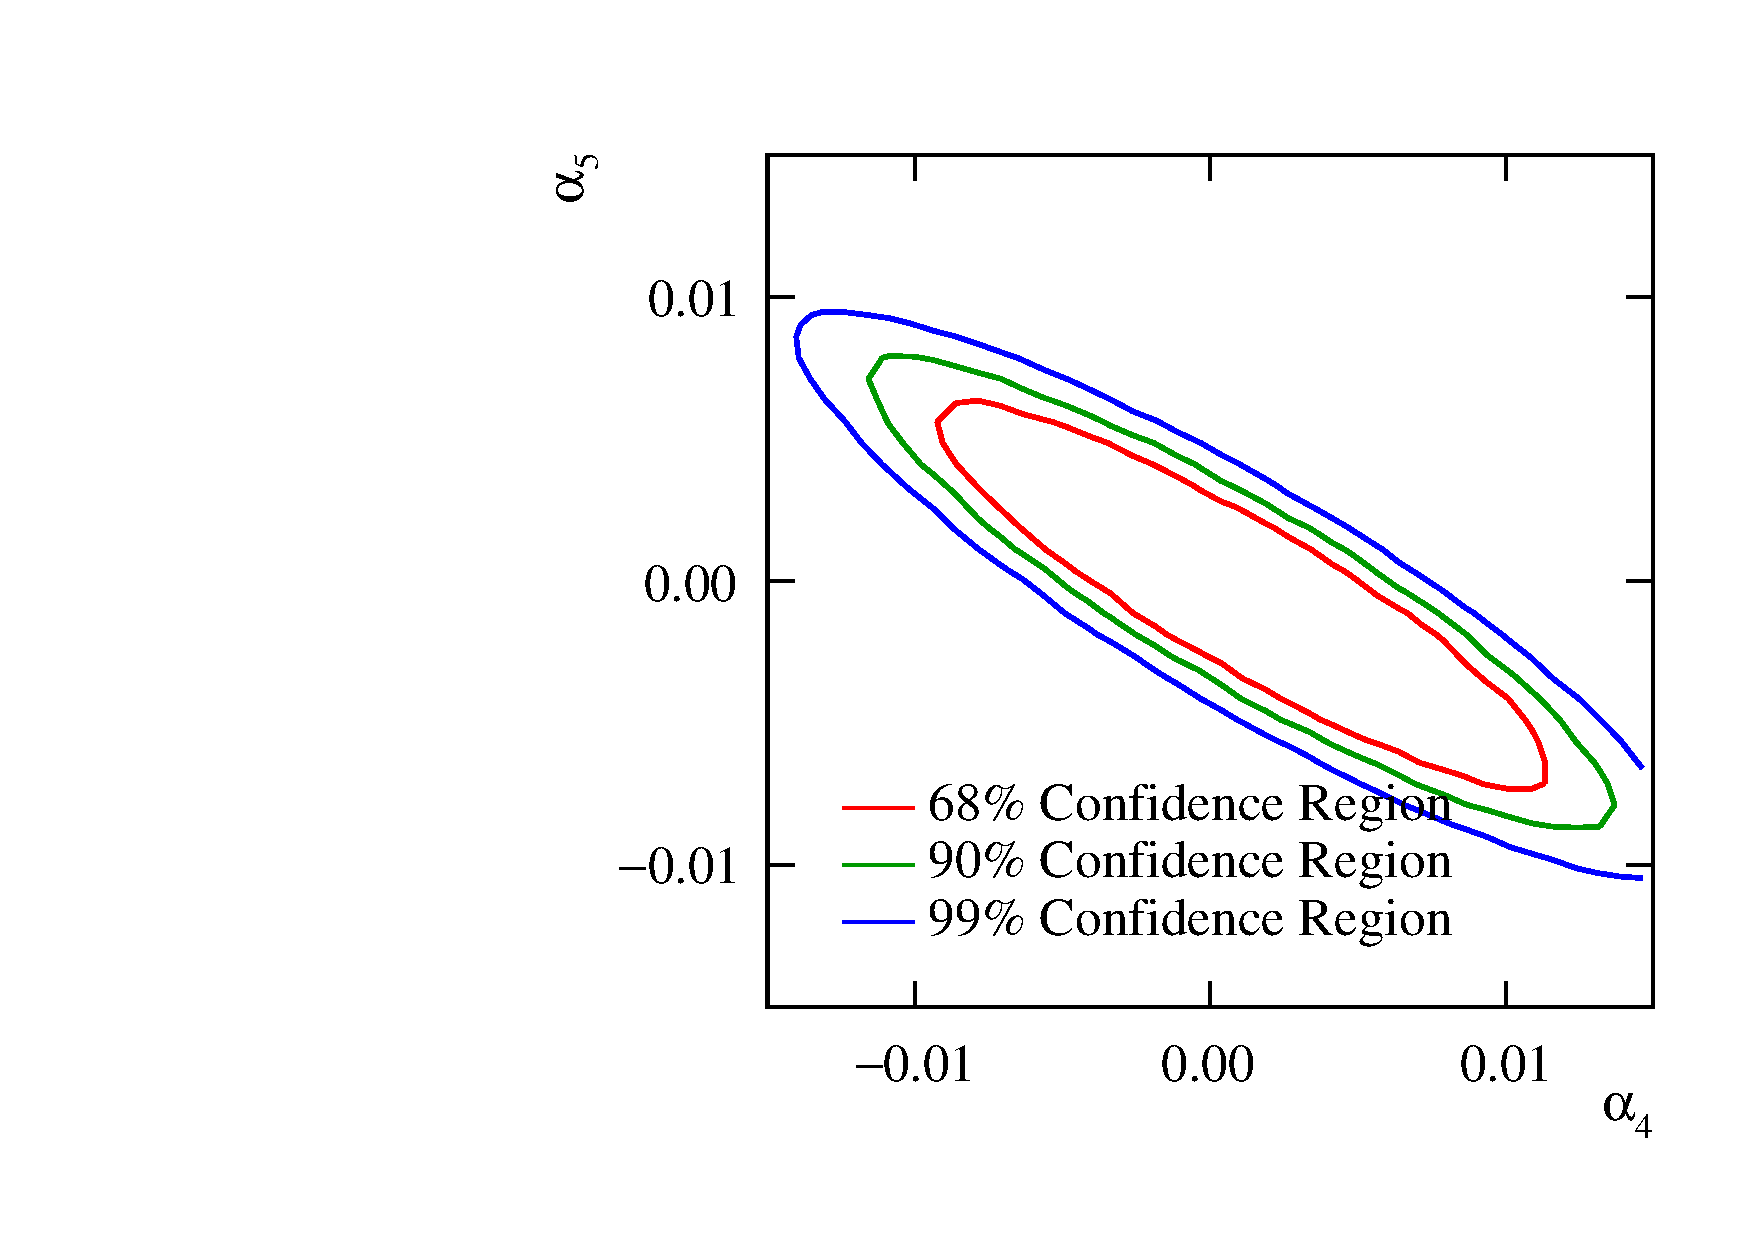
\includegraphics[width=0.5\textwidth]{PhysicsAnalysis/Plots/Chi2ContoursOptimisation/1400GeV/KtSPFOsR0p90.pdf}}\hfill
\subfloat[$\chi^{2}$ as a function of $\alpha_{4}$ assuming $\alpha_{5} = 0$.]{\label{fig:a4chi2jetalgoideal1400GeV}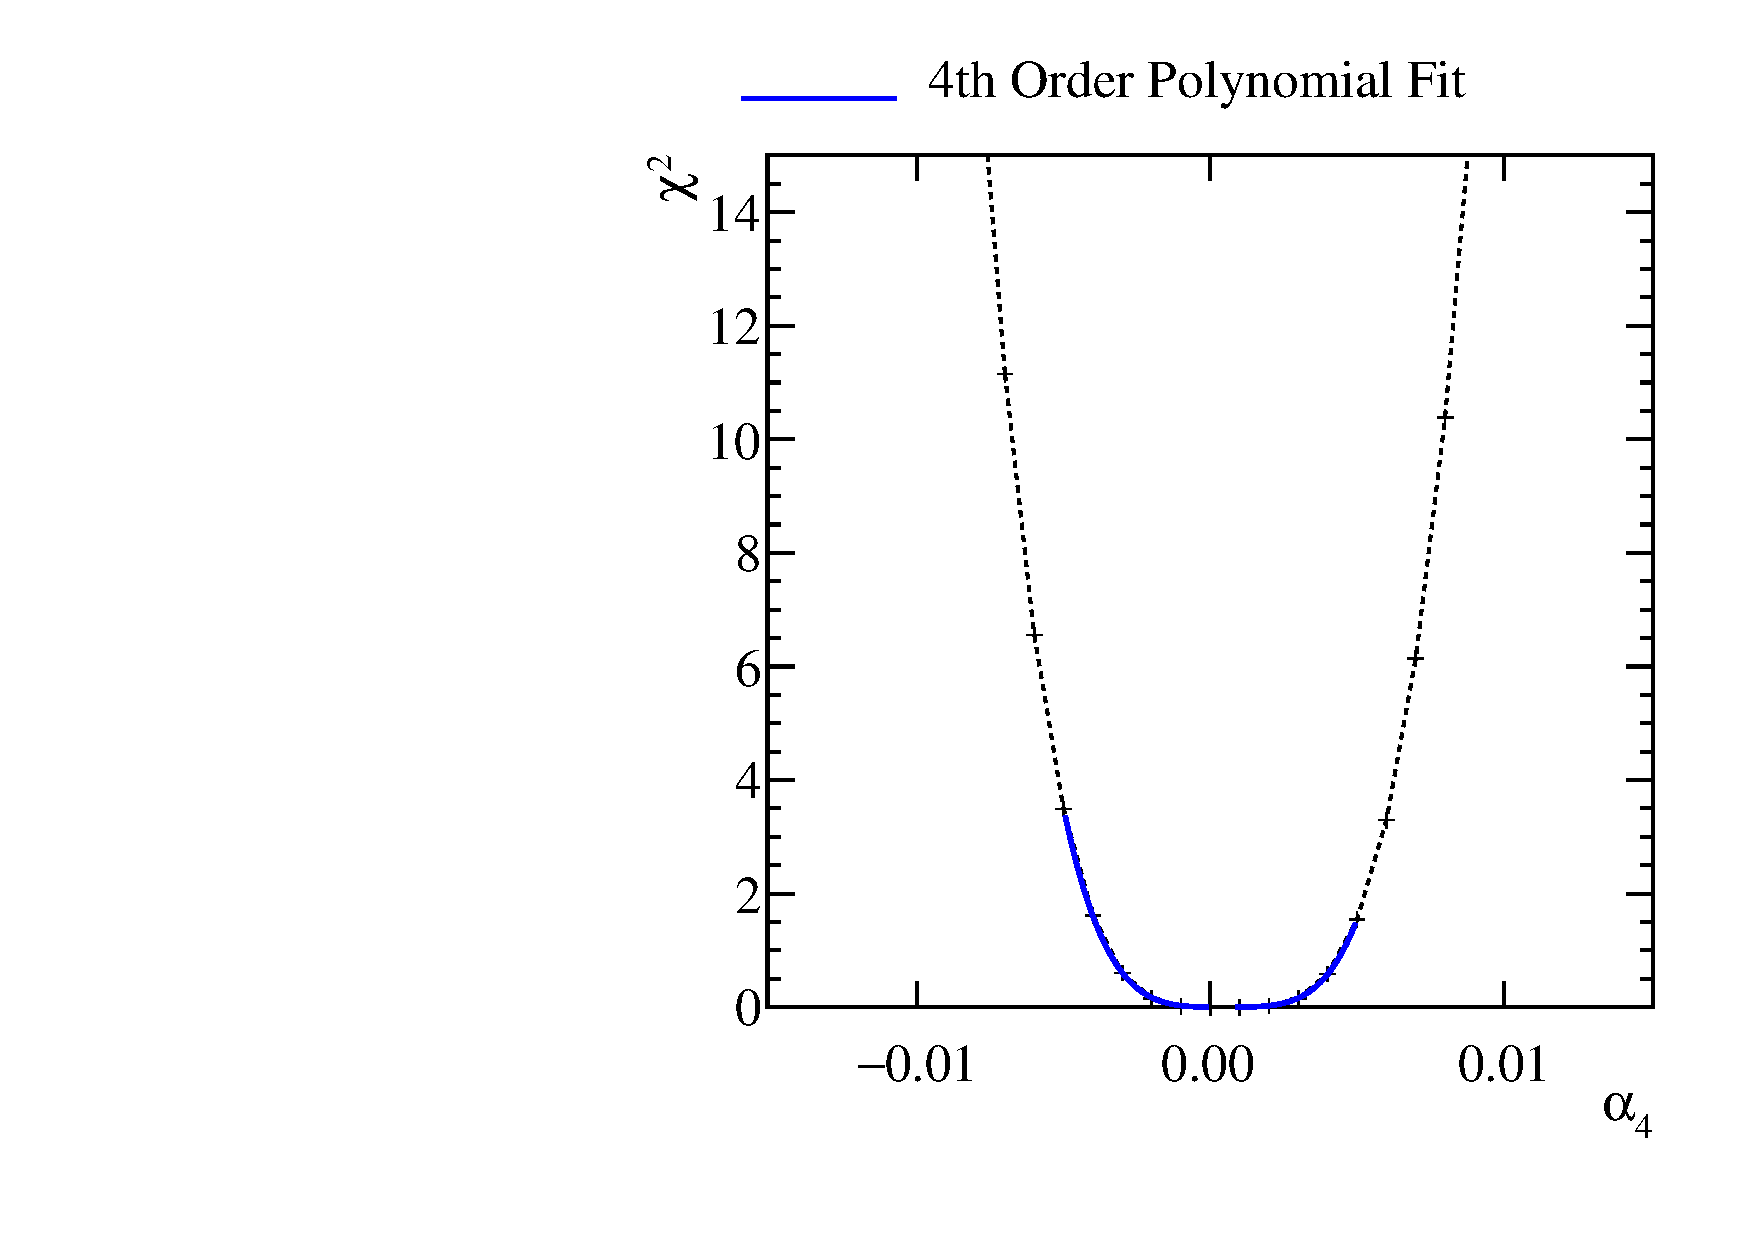
\includegraphics[width=0.5\textwidth]{PhysicsAnalysis/Plots/Chi2ContoursOptimisation/1400GeV/KtSPFOsR0p90_alpha4.pdf}}
\subfloat[$\chi^{2}$ as a function of $\alpha_{5}$ assuming $\alpha_{4} = 0$.]{\label{fig:a5chi2jetalgoideal1400GeV}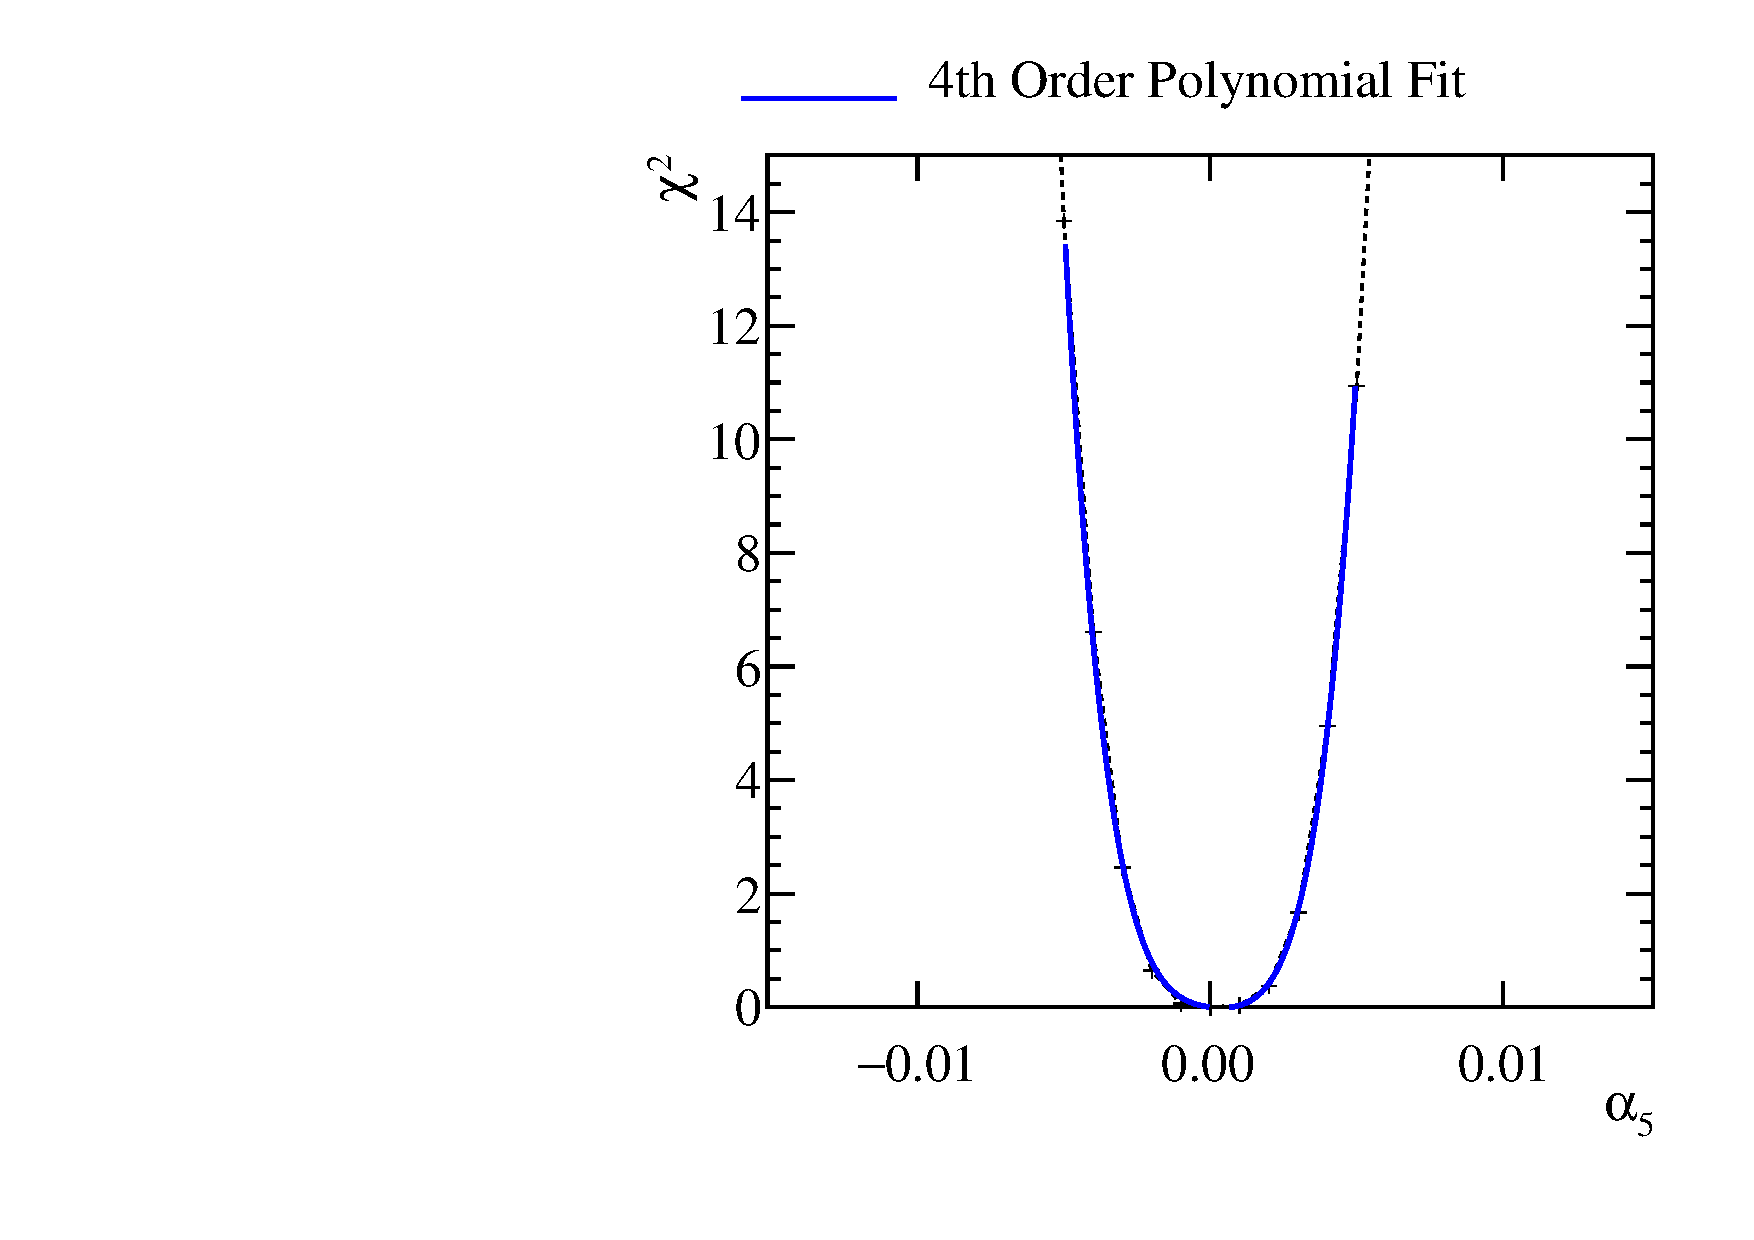
\includegraphics[width=0.5\textwidth]{PhysicsAnalysis/Plots/Chi2ContoursOptimisation/1400GeV/KtSPFOsR0p90_alpha5.pdf}}
\caption[$\chi^{2}$ sensitivity distributions for the $\text{qqqq}\nu\nu$ final state arising from a fit to $\text{cos}\theta^{*}_{\text{Jets}}$ at 1.4 TeV for the optimal jet reconstruction parameters.]{$\chi^{2}$ sensitivity distributions for the $\text{qqqq}\nu\nu$ final state arising from a fit to $\text{cos}\theta^{*}_{\text{Jets}}$ at 1.4 TeV for the optimal jet reconstruction parameters.} 
\label{fig:allchi2jetalgoideal1400GeV}
\end{figure}

\subsection{3 TeV Optimal Jet Reconstruction}
At 3 TeV the optimal sensitivity for the reconstructions considered is achieved for tight selected PFOs with an R parameter of 1.1 as can be seen from tables \ref{table:precisiona4signaljetalgo3000GeV} and \ref{table:precisiona5signaljetalgo3000GeV}.  The optimal contours can be found in figure \ref{fig:chi2jetalgoideal3000GeV} and the optimal 1D plot used to produce the errors references in the tables \ref{table:precisiona4signaljetalgo3000GeV} and \ref{table:precisiona5signaljetalgo3000GeV} can be found in figures \ref{fig:a4chi2jetalgoideal3000GeV} and \ref{fig:a5chi2jetalgoideal3000GeV} respectively.  All other contours and plots for this optimisation can be found in the appendices.  

The gains in optimising the jet algorithm at 3 TeV are larger than those found at 1.4 TeV.  The preference for the tight selected PFOs is to be expected as this configuration minimises the effect of beam induced backgrounds, which are more prominent at higher energies.  

\begin{table}[h!]
\centering
\begin{tabular}{l l l l}
\hline
PFO Selection & Tight Selected PFOs & Selected PFOs & Loose Selected PFOs \\ 
R Parameter & & & \\ 
\hline
0.7 & $-0.000529$ $+0.000525$ & $-0.000510$ $+0.000507$ & $-0.000547$ $+0.000555$ \\
0.9 & $-0.000566$ $+0.000555$ & $-0.000539$ $+0.000520$ & $-0.000568$ $+0.000553$ \\
1.1 & $-0.000472$ $+0.000472$ & $-0.000508$ $+0.000492$ & $-0.000504$ $+0.000489$ \\
\hline
\end{tabular}
\caption[$1\sigma$ precision on measurement of $\alpha_{4}$ for different jet reconstruction parameters considering pure signal at 3 TeV.]{Precision on measurement of $\alpha_{4}$ at 3 TeV for different jet reconstruction parameters considering pure signal and applying a $\chi^{2}$ fit to $\text{cos}\theta^{*}_{Jets}$.}
\label{table:precisiona4signaljetalgo3000GeV}
\end{table}

\begin{table}[h!]
\centering
\begin{tabular}{l l l l}
\hline
PFO Selection & Tight Selected PFOs & Selected PFOs & Loose Selected PFOs \\ 
R Parameter & & & \\ 
\hline
0.7 & $-0.000392$ $+0.000369$ & $-0.000355$ $+0.000348$ & $-0.000356$ $+0.000348$ \\
0.9 & $-0.000394$ $+0.000365$ & $-0.000391$ $+0.000361$ & $-0.000395$ $+0.000368$ \\
1.1 & $-0.000350$ $+0.000337$ & $-0.000374$ $+0.000354$ & $-0.000352$ $+0.000336$ \\
\hline
\end{tabular}
\caption[$1\sigma$ precision on measurement of $\alpha_{5}$ for different jet reconstruction parameters considering pure signal at 3 TeV.]{Precision on measurement of $\alpha_{5}$ at 3 TeV for different jet reconstruction parameters considering pure signal and applying a $\chi^{2}$ fit to $\text{cos}\theta^{*}_{Jets}$.}
\label{table:precisiona5signaljetalgo3000GeV}
\end{table}

\begin{figure}
\centering
\subfloat[$\chi^{2}$ sensitivity contours in $\alpha_{4}$ and $\alpha_{5}$ space.]{\label{fig:chi2jetalgoideal3000GeV}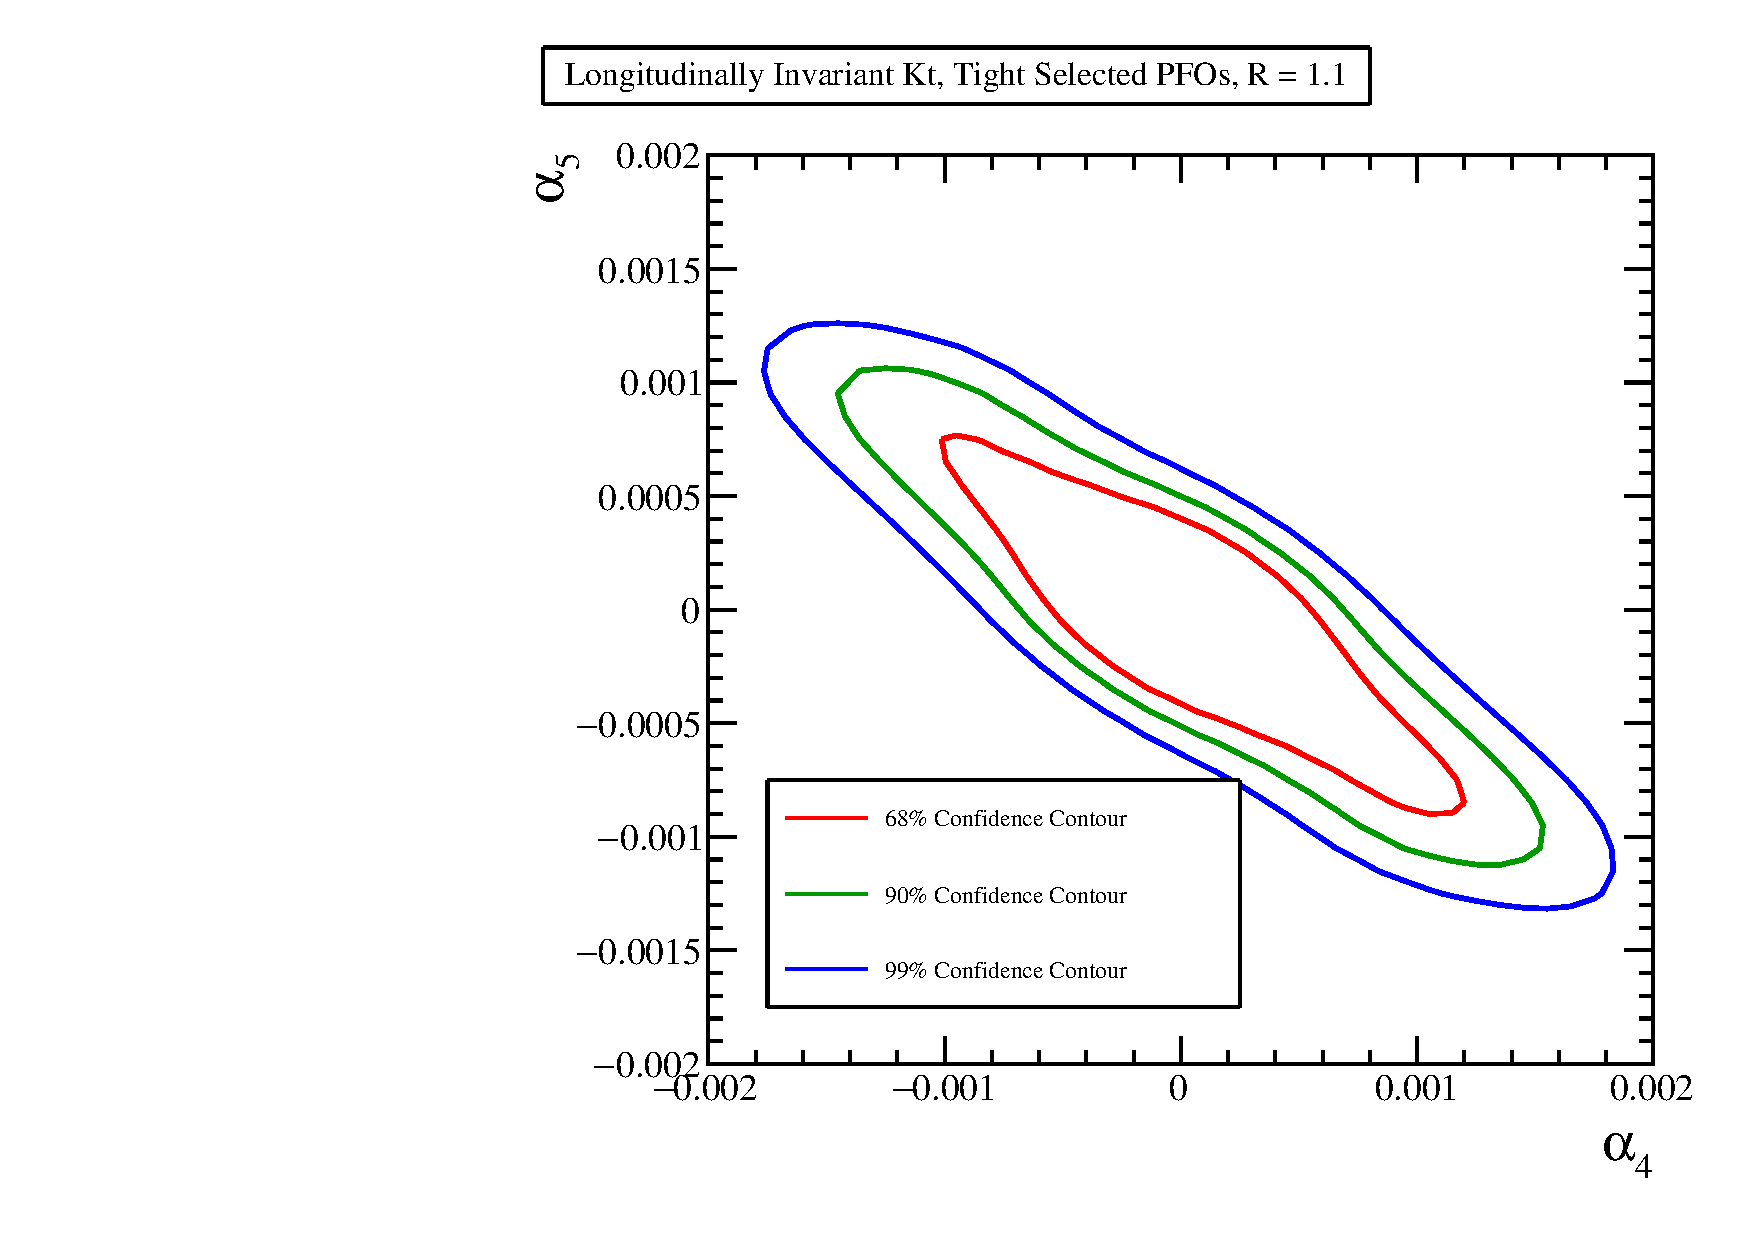
\includegraphics[width=0.5\textwidth]{PhysicsAnalysis/Plots/Chi2ContoursOptimisation/3000GeV/KtTPFOsR1p10.pdf}}\hfill
\subfloat[$\chi^{2}$ as a function of $\alpha_{4}$ assuming $\alpha_{5} = 0$.]{\label{fig:a4chi2jetalgoideal3000GeV}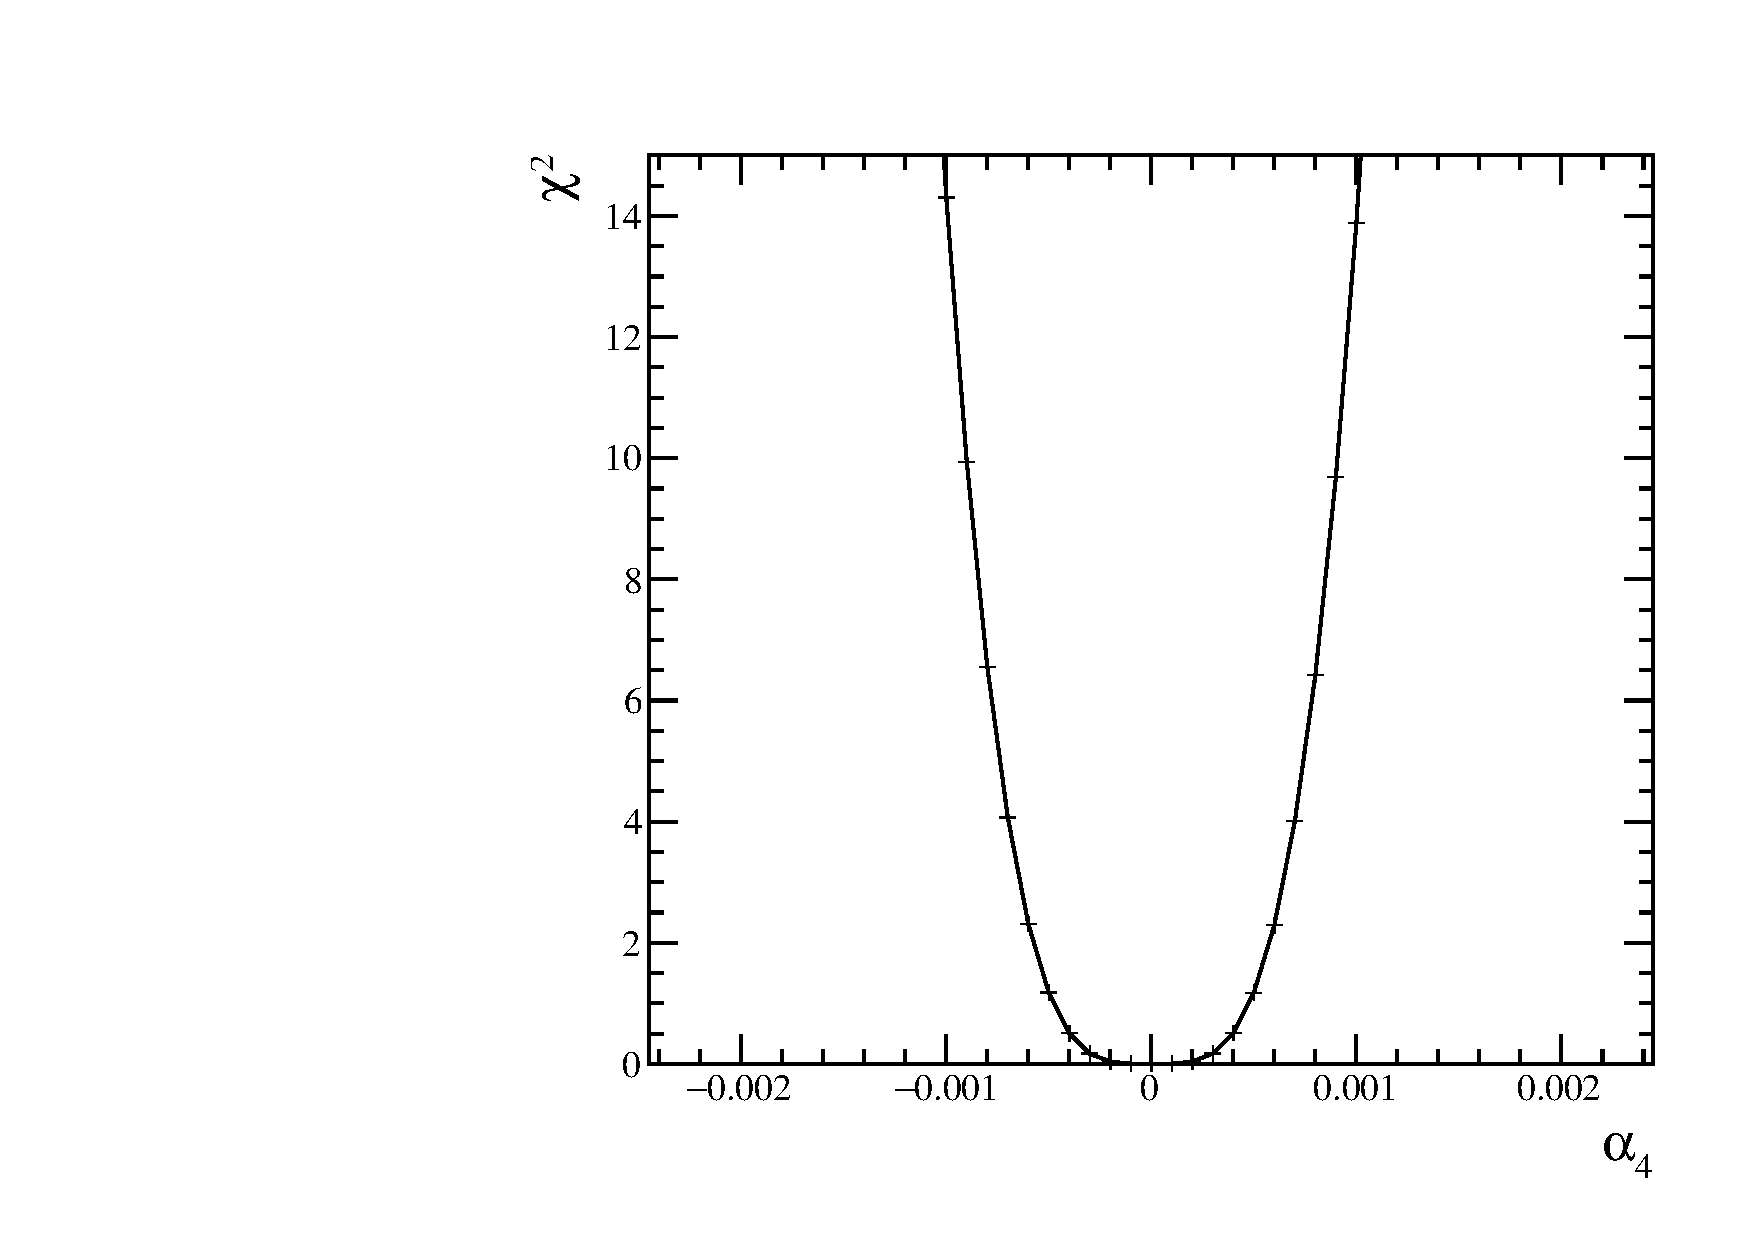
\includegraphics[width=0.5\textwidth]{PhysicsAnalysis/Plots/Chi2ContoursOptimisation/3000GeV/KtTPFOsR1p10_alpha4.pdf}}
\subfloat[$\chi^{2}$ as a function of $\alpha_{5}$ assuming $\alpha_{4} = 0$.]{\label{fig:a5chi2jetalgoideal3000GeV}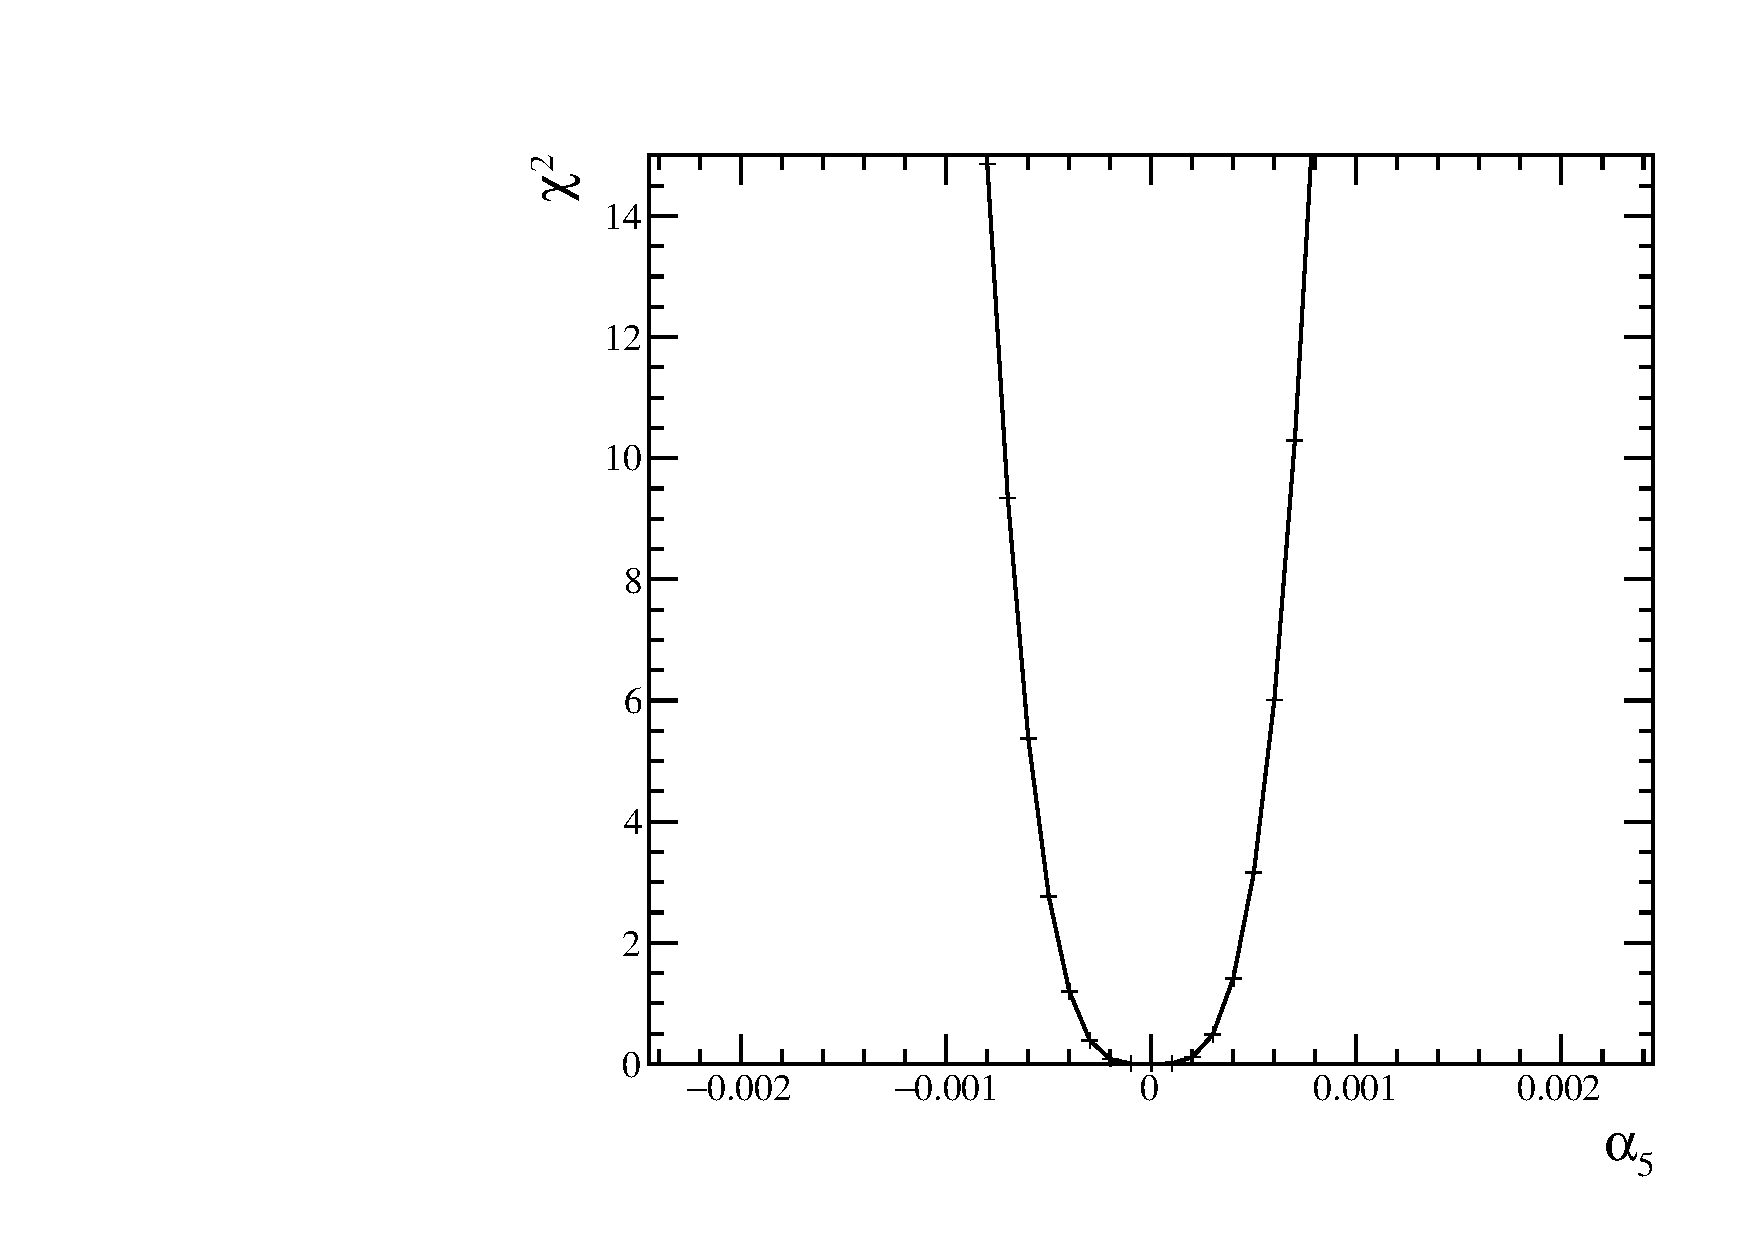
\includegraphics[width=0.5\textwidth]{PhysicsAnalysis/Plots/Chi2ContoursOptimisation/3000GeV/KtSPFOsR1p10_alpha5.pdf}}
\caption[$\chi^{2}$ sensitivity distributions for the $\text{qqqq}\nu\nu$ final state arising from a fit to $\text{cos}\theta^{*}_{\text{Jets}}$ at 3 TeV for the optimal jet reconstruction parameters.]{$\chi^{2}$ sensitivity distributions for the $\text{qqqq}\nu\nu$ final state arising from a fit to $\text{cos}\theta^{*}_{\text{Jets}}$ at 3 TeV for the optimal jet reconstruction parameters.} 
\label{fig:allchi2jetalgoideal3000GeV}
\end{figure}

\section{Event Selection}
As discussed earlier the signal events for this analysis contain the \nu{\nu}qqqq final state. The processes to be considered in this analysis alongside the signal are events that would topologically look similar to signal in the detector. This includes events that could be confused with 4 jet events with missing energy, while excluding those events with large numbers of high energy leptons that could be vetoed easily during the analysis stage. In full the list includes:

\begin{table}[h!]
\centering
\begin{tabular}{ l l l}
\hline
Final State & Cross Section 1.4 TeV [fb] & Cross Section 3 TeV [fb]  \\ 
\hline
$\text{e}^{+}\text{e}^{-} \rightarrow \nu{\nu}\text{qqqq}$ & 24.7 & 71.5 \\
$\text{e}^{+}\text{e}^{-} \rightarrow \text{l}\nu\text{qqqq}$ & 110.4 & 106.6 \\
$\text{e}^{+}\text{e}^{-} \rightarrow \text{llqqqq}$ & 62.1 & 169.3 \\
$\text{e}^{+}\text{e}^{-} \rightarrow \text{qqqq}$ & 1245.1 & 546.5 \\
$\text{e}^{+}\text{e}^{-} \rightarrow \nu{\nu}\text{qq}$ & 787.7 & 1317.5 \\
$\text{e}^{+}\text{e}^{-} \rightarrow \text{l}\nu\text{qq}$ & 4309.7 & 5560.9 \\
$\text{e}^{+}\text{e}^{-} \rightarrow \text{llqq}$ & 2725.8 & 3319.6 \\
$\text{e}^{+}\text{e}^{-} \rightarrow \text{qq}$ & 4009.5 & 2948.9 \\
$\gamma_{\text{EPA}}\text{e}^{-} \rightarrow \text{qqqq}\text{e}^{-}$ & 287.1 & 287.8 \\
$\gamma_{\text{BS}}\text{e}^{-} \rightarrow \text{qqqq}\text{e}^{-}$ & 1160.7 & 1268.6 \\
$\text{e}^{+}\gamma_{\text{EPA}} \rightarrow \text{qqqq}\text{e}^{+}$ & 286.9 & 287.8 \\
$\text{e}^{+}\gamma_{\text{BS}} \rightarrow \text{qqqq}\text{e}^{+}$ & 1156.3 & 1267.3 \\
$\gamma_{\text{EPA}}\text{e}^{-} \rightarrow \text{qqqq}\nu$ & 32.6 & 54.2 \\
$\gamma_{\text{BS}}\text{e}^{-} \rightarrow \text{qqqq}\nu$ & 136.9 & 262.5 \\
$\text{e}^{+}\gamma_{\text{EPA}} \rightarrow \text{qqqq}\nu$ & 32.6 & 54.2 \\
$\text{e}^{+}\gamma_{\text{BS}} \rightarrow \text{qqqq}\nu$ & 136.4 & 262.3 \\
$\gamma_{\text{EPA}}\gamma_{\text{EPA}} \rightarrow \text{qqqq}$ & 753.0 & 402.7 \\
$\gamma_{\text{EPA}}\gamma_{\text{BS}} \rightarrow \text{qqqq}$ & 4034.8 & 2423.1 \\
$\gamma_{\text{BS}}\gamma_{\text{EPA}} \rightarrow \text{qqqq}$ & 4018.7 & 2420.6 \\
$\gamma_{\text{BS}}\gamma_{\text{BS}} \rightarrow \text{qqqq}$ & 21406.2 & 13050.3 \\
\hline
\end{tabular}
\caption[]{Cross sections of signal and background processes at 1.4 and 3 TeV. In the above table q $\in$ u, $\bar{\text{u}}$, d, $\bar{\text{d}}$, s, $\bar{\text{s}}$, c, $\bar{\text{c}}$, b or $\bar{\text{b}}$ while l $\in$ $\text{e}^{\pm}$, $\mu^{\pm}$ or $\tau^{\pm}$ and $\nu$ $\in$ $\nu_{e}$, $\nu_{\mu}$ and $\nu_{\tau}$.  The subscript EPA or BS for the incoming photons indicate whether the photon is generated from the equivalent photon approximation or beamstrahlung.}
\label{table:crosssectionfull}
\end{table}

Equivalent Photon Approximation (EPA) processes model the electromagnetic field of a charged particle as virtual photons.  BS (beamstrahlung) processes involve photons that have been radiated from incoming charged particles due to interactions with the electromagnetic field of the opposite beam.   The energy spectrum of the incoming particles for CLIC at the relevant operating energy is used to model the energy of these incoming photons.  Included in this study are photon-photon interactions from photons appearing from the EPA and beamstrahlung processes.

\subsection{Pre Selection - 1.4 TeV}
\label{sec:preselection1400GeV}
The primary selection of the \nu{\nu}qqqq signal will be done using a multivariate analysis, however, in an attempt to veto trivial backgrounds a simple cut based preselection is applied. Cuts are applied to the transverse momentum, invariant mass of the visible system and the number of isolated leptons. The raw distributions of these variables is
shown in figure \ref{fig:preselection1400}. Based on these distributions the following cuts were applied:

\begin{itemize}
\item Transverse momentum > 100 GeV. This cut is effective due to the presence of missing energy in the form of neutrinos in the signal final state.
\item Visible mass of the system > 200 GeV. This cut is effective for accounting for the missing energy of the neutrinos in the final state along the longitudinal direction of the detector instead.
\item Number of isolated leptons = 0. This cut vetoes a large number of events with leptons in the final state.
The effect of these preselection cuts can be found in table 1.3. While a large fraction of the signal events are lost through these cuts, particularly the transverse momentum cuts, a much large fraction of background events are removed justifying the cut.
\end{itemize}

The event numbers for the signal and background are shown in table \ref{table:preselectionnumbers1400GeV} as these cuts are cumulatively applied.  These numbers are normalised to the correct luminosity for CLIC running at 1.4 TeV.  As is expected the large transverse momentum cut removes practically all backgrounds containing no missing energy.  The invariant mass cut removes significant fractions of two quark and missing energy events.  Finally, the isolated lepton finder cut removes backgrounds containing visible leptonic final states.  

\begin{table}[h!]
\centering
\begin{tabular}{ l l l l l}
\hline
Final State & Raw Event  & $p_{T}$ > 100 GeV & $p_{T}$ > 100 GeV \& & $p_{T}$ > 100 GeV \& \\ 
& Numbers & & $M_{\text{Vis}}$ > 200 GeV & $M_{\text{Vis}}$ > 200 GeV \&\\ 
& & & & $N_{\text{Isolated Leptons}}$ = 0\\ 
\hline
$\text{e}^{+}\text{e}^{-} \rightarrow \nu{\nu}\text{qqqq}$ & 37,050 & 23,800 & 21,080 & 21,020\\
$\text{e}^{+}\text{e}^{-} \rightarrow \text{l}\nu\text{qqqq}$ & 165,600 & 81,620 & 80,840 & 42,410\\
$\text{e}^{+}\text{e}^{-} \rightarrow \text{llqqqq}$ & 93,150 & 1,151 & 1,140 & 700\\
$\text{e}^{+}\text{e}^{-} \rightarrow \text{qqqq}$ & 1,868,000 & 6,487 & 6,467 & 6,445\\
$\text{e}^{+}\text{e}^{-} \rightarrow \nu{\nu}\text{qq}$ & 1,181,000 & 514,100 & 50,260 & 50,150\\
$\text{e}^{+}\text{e}^{-} \rightarrow \text{l}\nu\text{qq}$ & 6,464,000 & 2,003,000 & 1,259,000 & 567,600\\
$\text{e}^{+}\text{e}^{-} \rightarrow \text{llqq}$ & 4,088,000 & 7,754 & 7,351 & 5,643\\
$\text{e}^{+}\text{e}^{-} \rightarrow \text{qq}$ & 6,011,000 & 34,610 & 34,130 & 34,070\\
$\gamma_{\text{EPA}}\text{e}^{-} \rightarrow \text{qqqq}\text{e}^{-}$ & 430,600 & 2,463 & 2,446 & 865\\
$\gamma_{\text{BS}}\text{e}^{-} \rightarrow \text{qqqq}\text{e}^{-}$ & 1,306,000 & 1,382 & 1,340 & 1,002\\
$\text{e}^{+}\gamma_{\text{EPA}} \rightarrow \text{qqqq}\text{e}^{+}$ & 430,300 & 2,846 & 2,823 & 1,121\\
$\text{e}^{+}\gamma_{\text{BS}} \rightarrow \text{qqqq}\text{e}^{+}$ & 1,301,000 & 654 & 643 & 469\\
$\gamma_{\text{EPA}}\text{e}^{-} \rightarrow \text{qqqq}\nu$ & 48,890 & 17,450 & 13,490 & 8,852\\
$\gamma_{\text{BS}}\text{e}^{-} \rightarrow \text{qqqq}\nu$ & 154,000 & 56,380 & 36,350 & 35,900\\
$\text{e}^{+}\gamma_{\text{EPA}} \rightarrow \text{qqqq}\nu$ & 48,890 & 17,520 & 13,550 & 8,928\\
$\text{e}^{+}\gamma_{\text{BS}} \rightarrow \text{qqqq}\nu$ & 153,400 & 56,280 & 36,340 & 35,900\\
$\gamma_{\text{EPA}}\gamma_{\text{EPA}} \rightarrow \text{qqqq}$ & 1,129,000 & 3,160 & 3,079 & 1,563\\
$\gamma_{\text{EPA}}\gamma_{\text{BS}} \rightarrow \text{qqqq}$ & 4,539,000 & 5,325 & 5,270 & 3,987\\
$\gamma_{\text{BS}}\gamma_{\text{EPA}} \rightarrow \text{qqqq}$ & 4,521,000 & 3,810 & 3,730 & 2,318\\
$\gamma_{\text{BS}}\gamma_{\text{BS}} \rightarrow \text{qqqq}$ & 20,550,000 & 2,445 & 2,445 & 1,673\\
\hline
\end{tabular}
\caption[Number of events passing the various cuts applied in the preselection at 1.4TeV.]{Number of events passing the various cuts applied in the preselection at 1.4TeV.  Event numbers are normalised to the correct luminosity for CLIC at 1.4 TeV.  $p_{T}$ is the transverse momentum of the event,  $M_{\text{Vis}}$ is the visible mass and $N_{\text{Isolated Leptons}}$ is the number of isolated leptons in the event.  In the above table q $\in$ u, $\bar{\text{u}}$, d, $\bar{\text{d}}$, s, $\bar{\text{s}}$, c, $\bar{\text{c}}$, b or $\bar{\text{b}}$ while l $\in$ $\text{e}^{\pm}$, $\mu^{\pm}$ or $\tau^{\pm}$ and $\nu$ $\in$ $\nu_{e}$, $\nu_{\mu}$ and $\nu_{\tau}$.  The subscript EPA or BS for the incoming photons indicate whether the photon is generated from the equivalent photon approximation or beamstrahlung.}
\label{table:preselectionnumbers1400GeV}
\end{table}

\begin{figure}
\centering
\subfloat[Transverse momentum of system.]{\label{fig:preselection1400_1}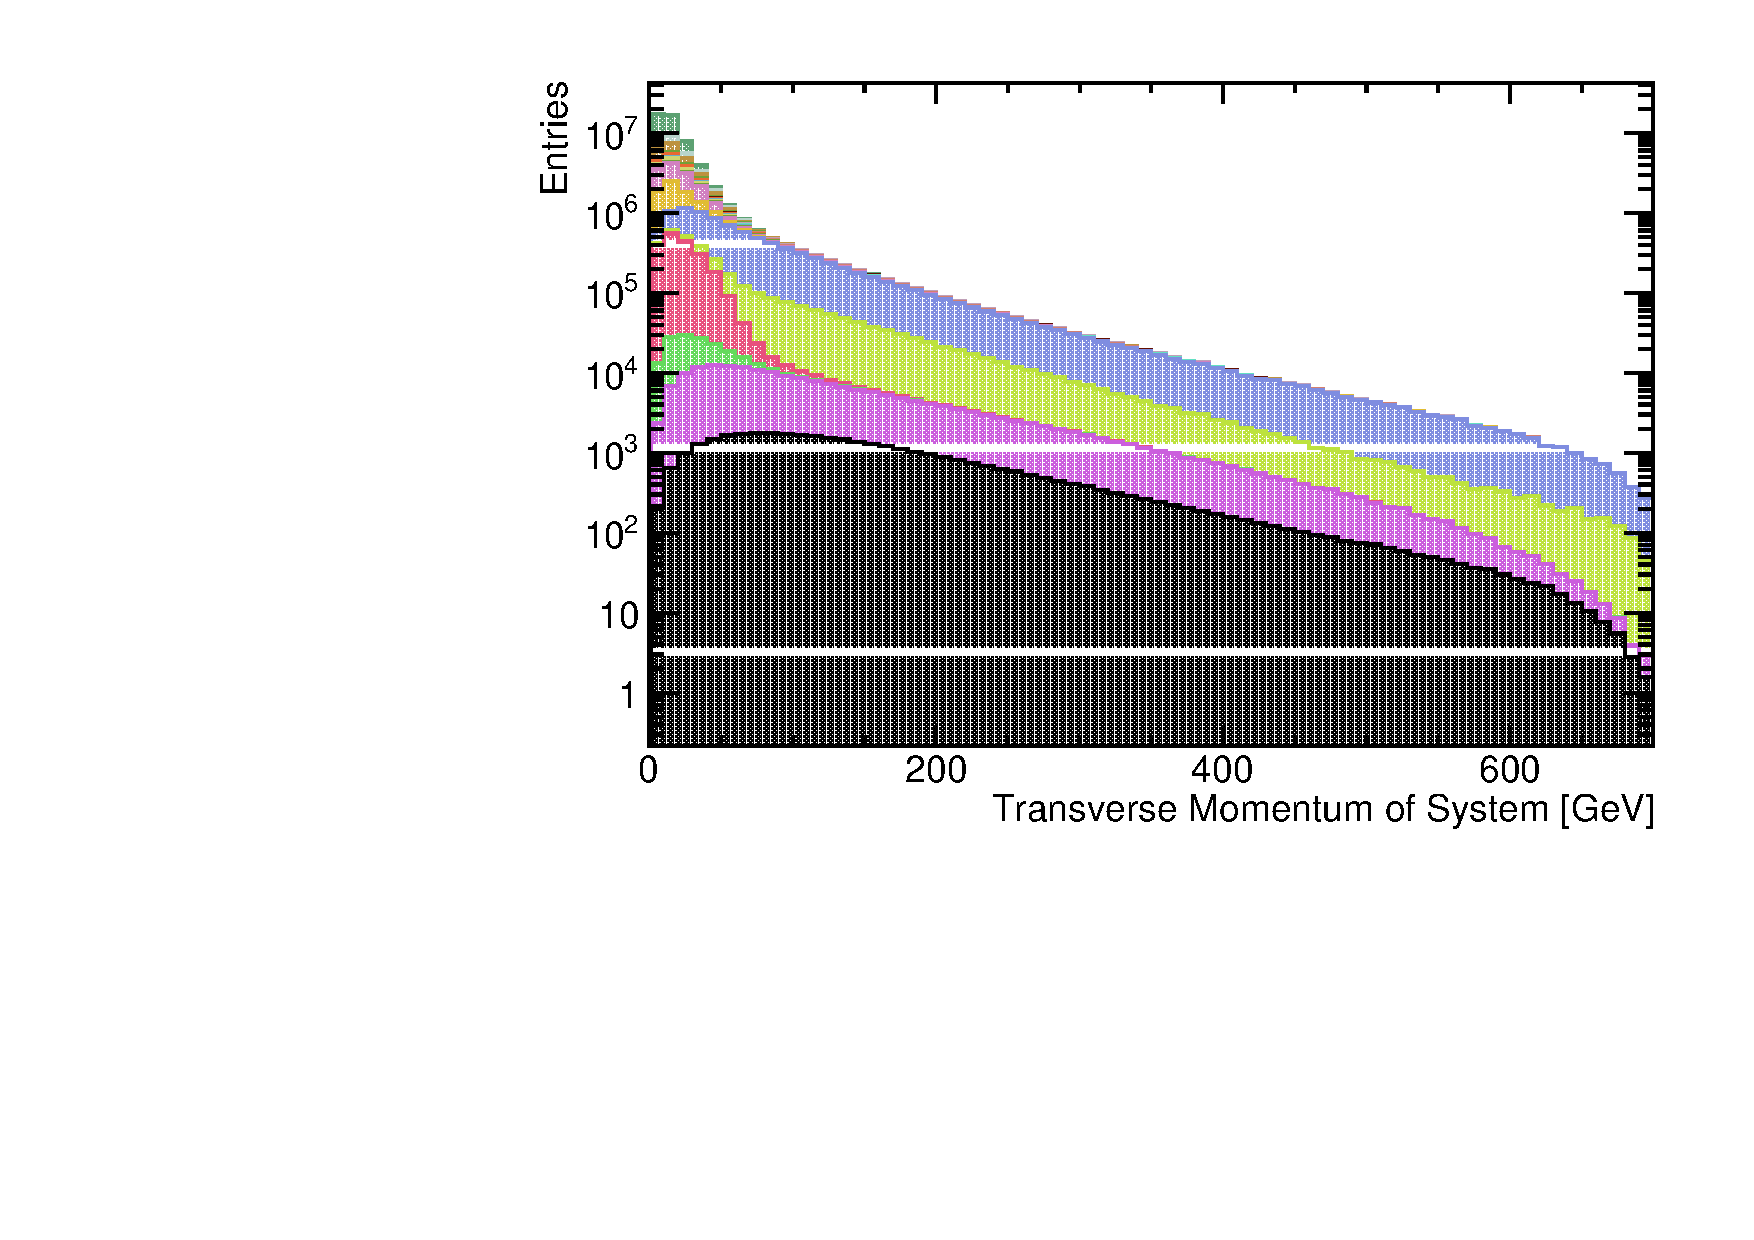
\includegraphics[width=0.5\textwidth]{PhysicsAnalysis/Plots/PreSelection/1400GeV/TransverseMomentum.pdf}}\hfill
\subfloat[Invariant mass of the visible system.]{\label{fig:preselection1400_2}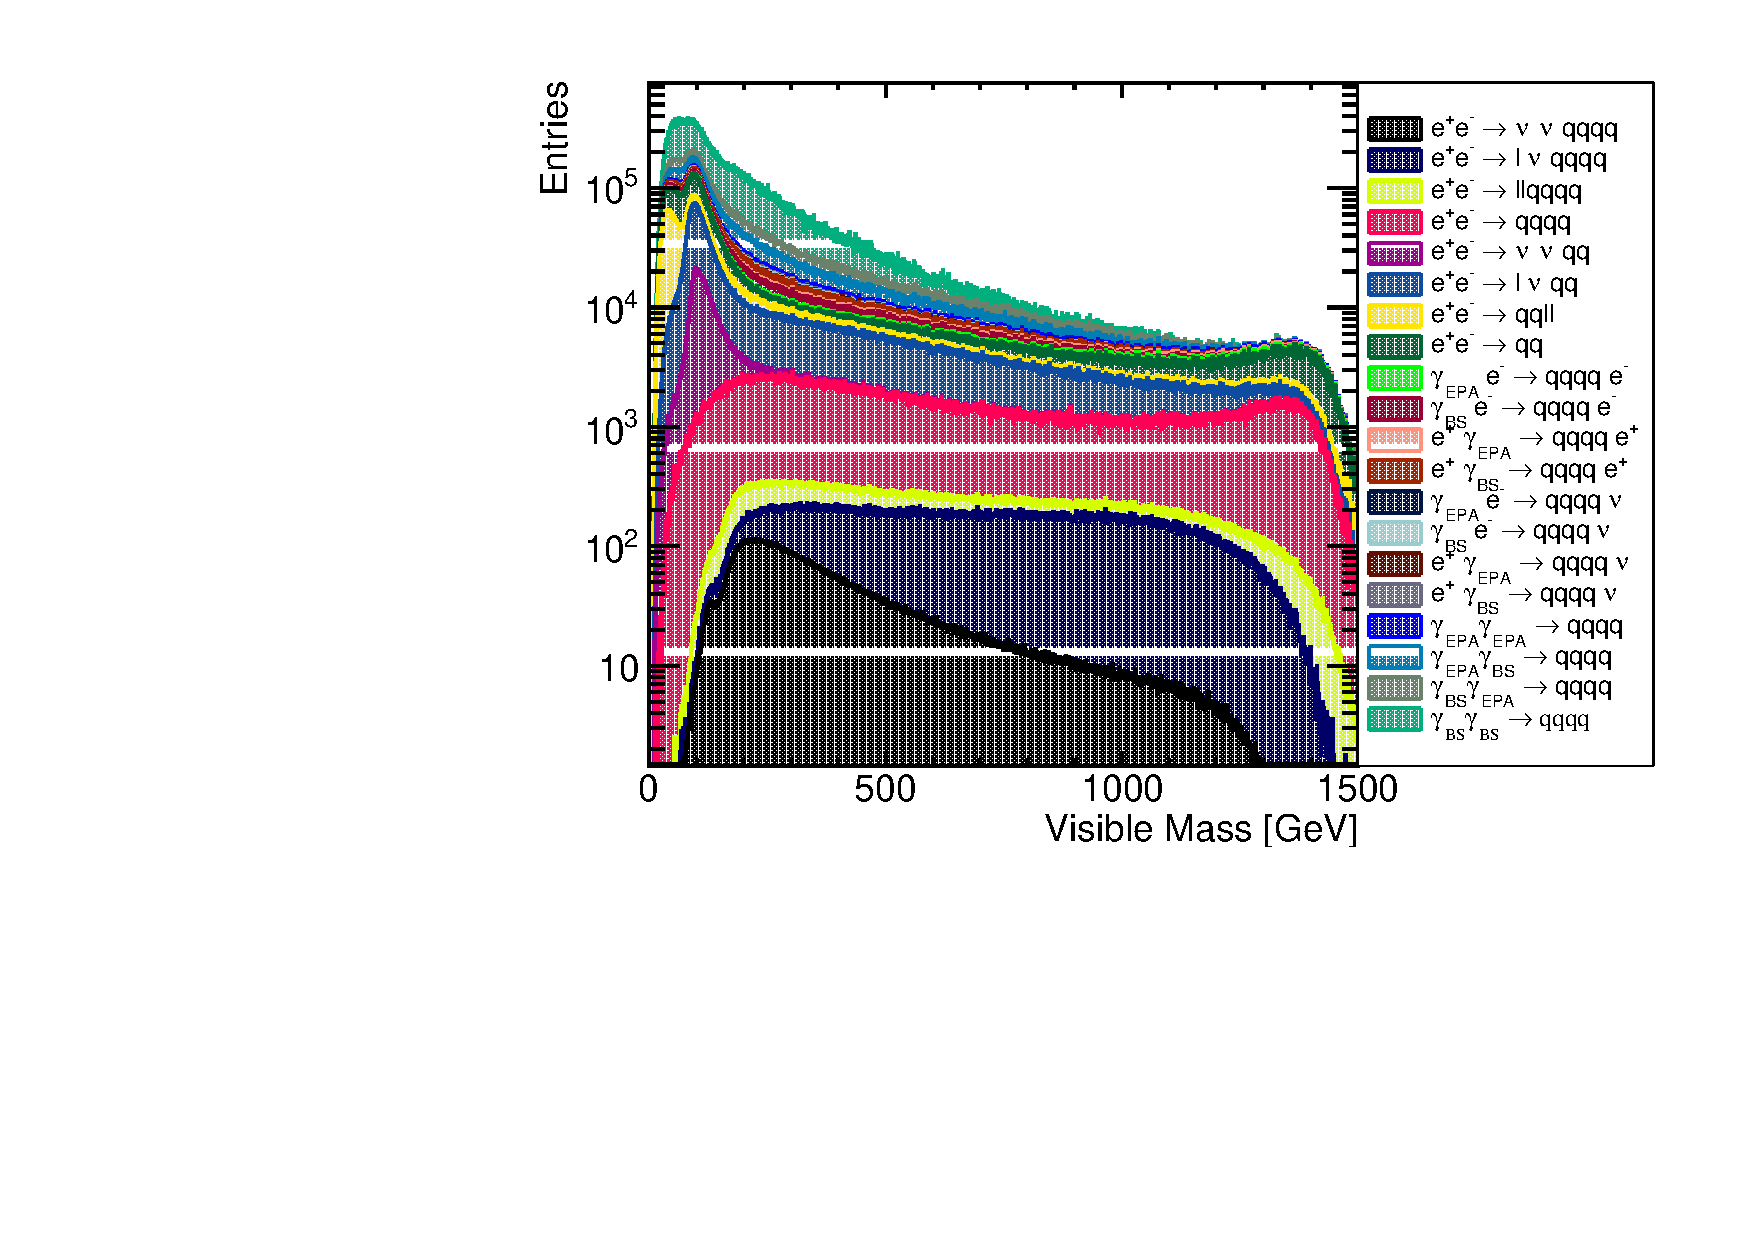
\includegraphics[width=0.5\textwidth]{PhysicsAnalysis/Plots/PreSelection/1400GeV/InvariantMassSystem.pdf}}
\subfloat[Number of isolated leptons.]{\label{fig:preselection1400_3}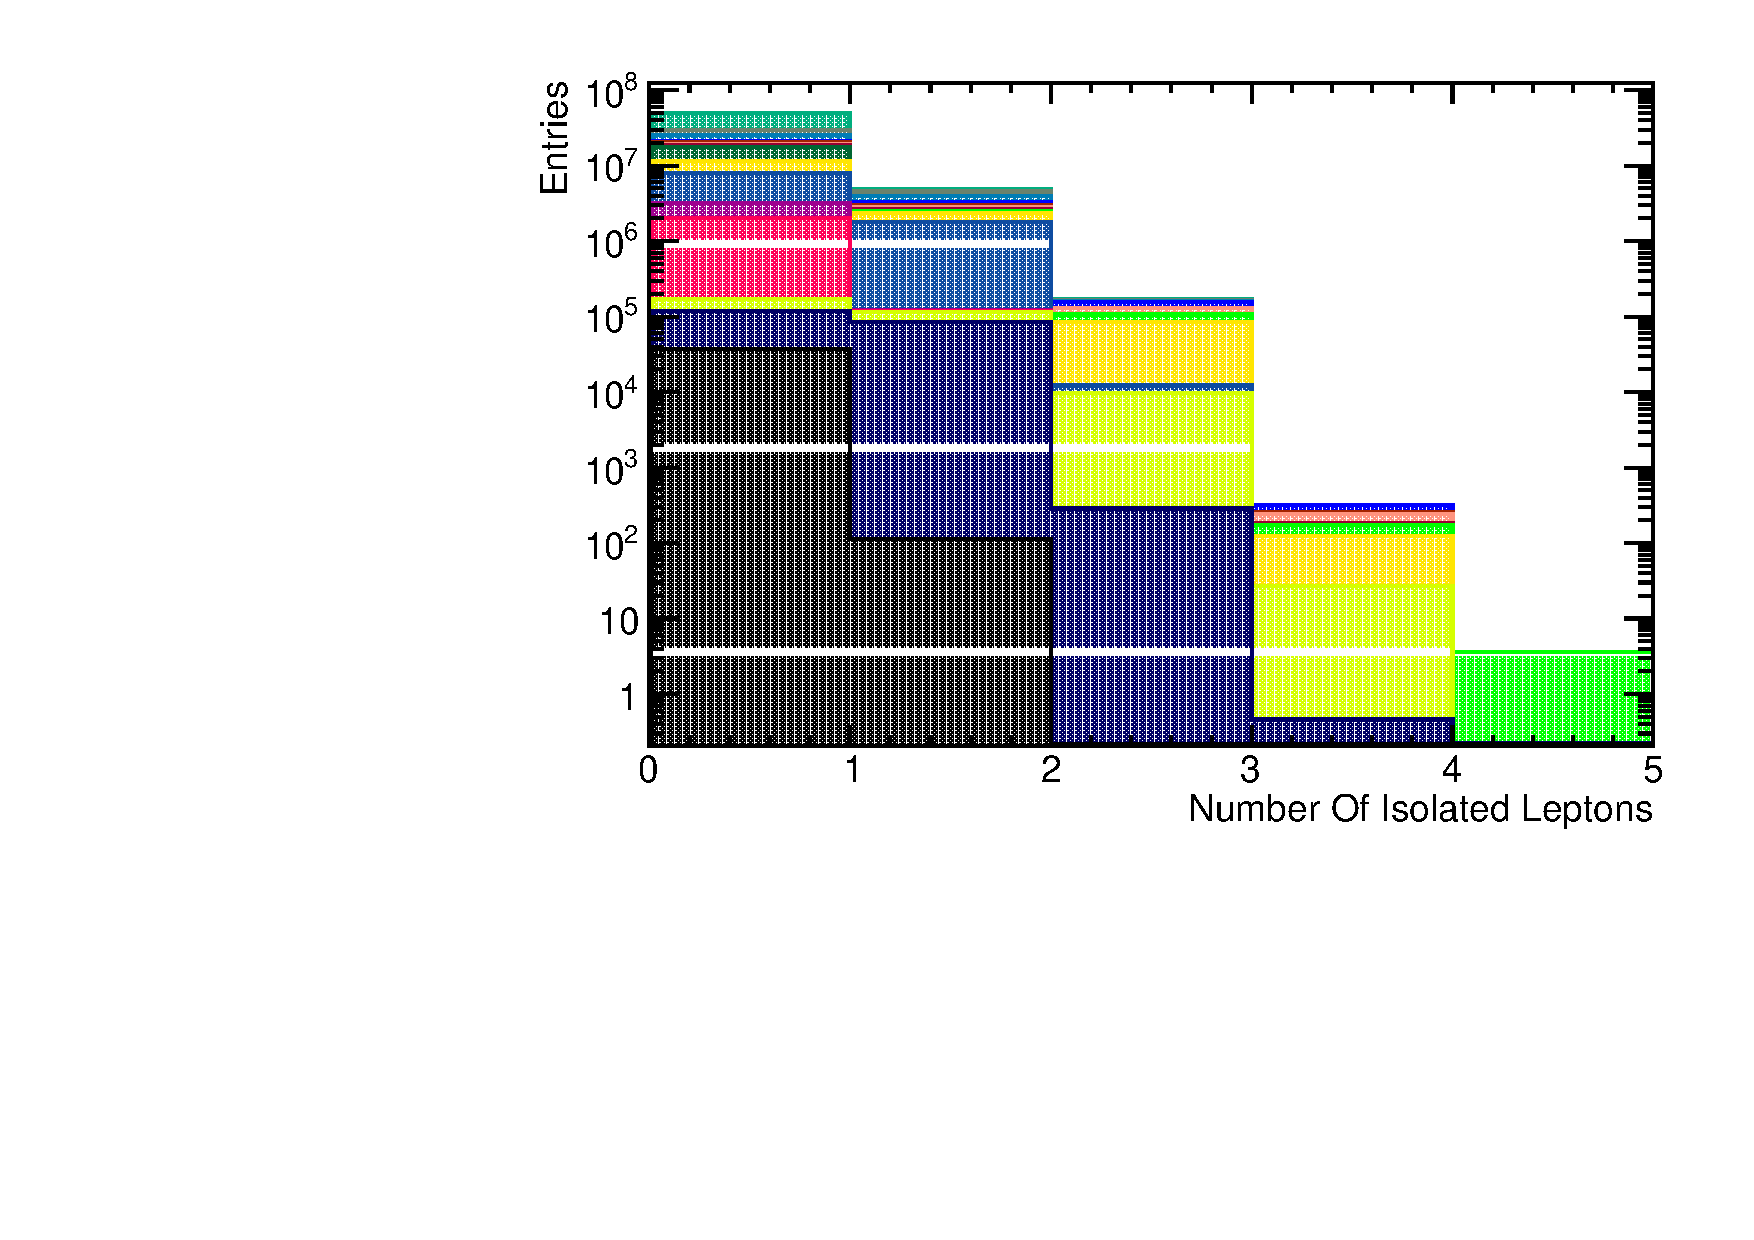
\includegraphics[width=0.5\textwidth]{PhysicsAnalysis/Plots/PreSelection/1400GeV/NumberOfIsolatedLeptons.pdf}}
\caption[Distribution of variables cut on in the preselection at 1.4 TeV.]{Distribution of variables cut on in the preselection at 1.4 TeV.}
\label{fig:preselection1400}
\end{figure}

\subsection{MVA - 1.4 TeV}
\label{sec:mva1400GeV}
A multivariate analysis was applied to the data set to refine the selection using the TMVA toolkit \cite{Hocker:2007ht}. The following variables were used for training the TMVA selection.  

\begin{itemize}
\item Number of PFOs in the event.
\item Highest energy PFO type.
\item Transverse momentum of the event.
\item $\text{cos}\theta_{Missing}$.  The cosine of the polar angle of the missing momentum.
\item $\text{cos}\theta_{\text{Highest Energy Track}}$.  The cosine of the polar angle of the track with the largest momentum.
\item $y_{i}$, $y_{i+1}$. Jet clustering parameters ranging from i = 0 to 6.
\item Principle thrust, sphericity and aplanarity as defined in section BLAH.
\item Energy of the highest energy electron in the event.
\item Energy of the highest energy PFO in the event.
\item Energy of the reconstructed bosons.
\item Acolinearity of the reconstructed boson pair.
\item Invariant mass of the reconstructed bosons.
\item Acolinearity of the jets forming the reconstructed bosons. 
\end{itemize}

It was found that the best MVA algorithm for both performance and speed was the booted decision tree (BDT) when comparing different methods using the default settings.  Add plot here.

The BDT was further optimised by varying the number of trees used, the depth of the trees and the number of cuts applied.  The results shown in the rest of this section use the optimal configuration.  For the optimal BDT configuration a significance of S/$\sqrt(\text{S + B}) = 53.6$ was obtained.  

The event numbers passing the BDT cut can be found in table \ref{table:postmvanumbers1400GeV}.  The performance of the BDT is shown in figure \ref{fig:synbosonmass1400GeVMVAimpact}, which shows the change in the distribution of the the invariant mass of the reconstructed bosons as the MVA is applied. As expected the dominant background processes after the MVA is applied are those that will look identical to the visible signal process i.e. qqqq and missing energy.  Two smaller sources of background that pass the MVA exists, those where two jets and missing energy are confused as four jets and missing energy and those where a lepton is not properly reconstructed and the events look like four jets and missing energy.  

\begin{figure}
\centering
\subfloat[No cuts applied.]{\label{fig:nocutssynbosonmass1400GeVMVAimpact}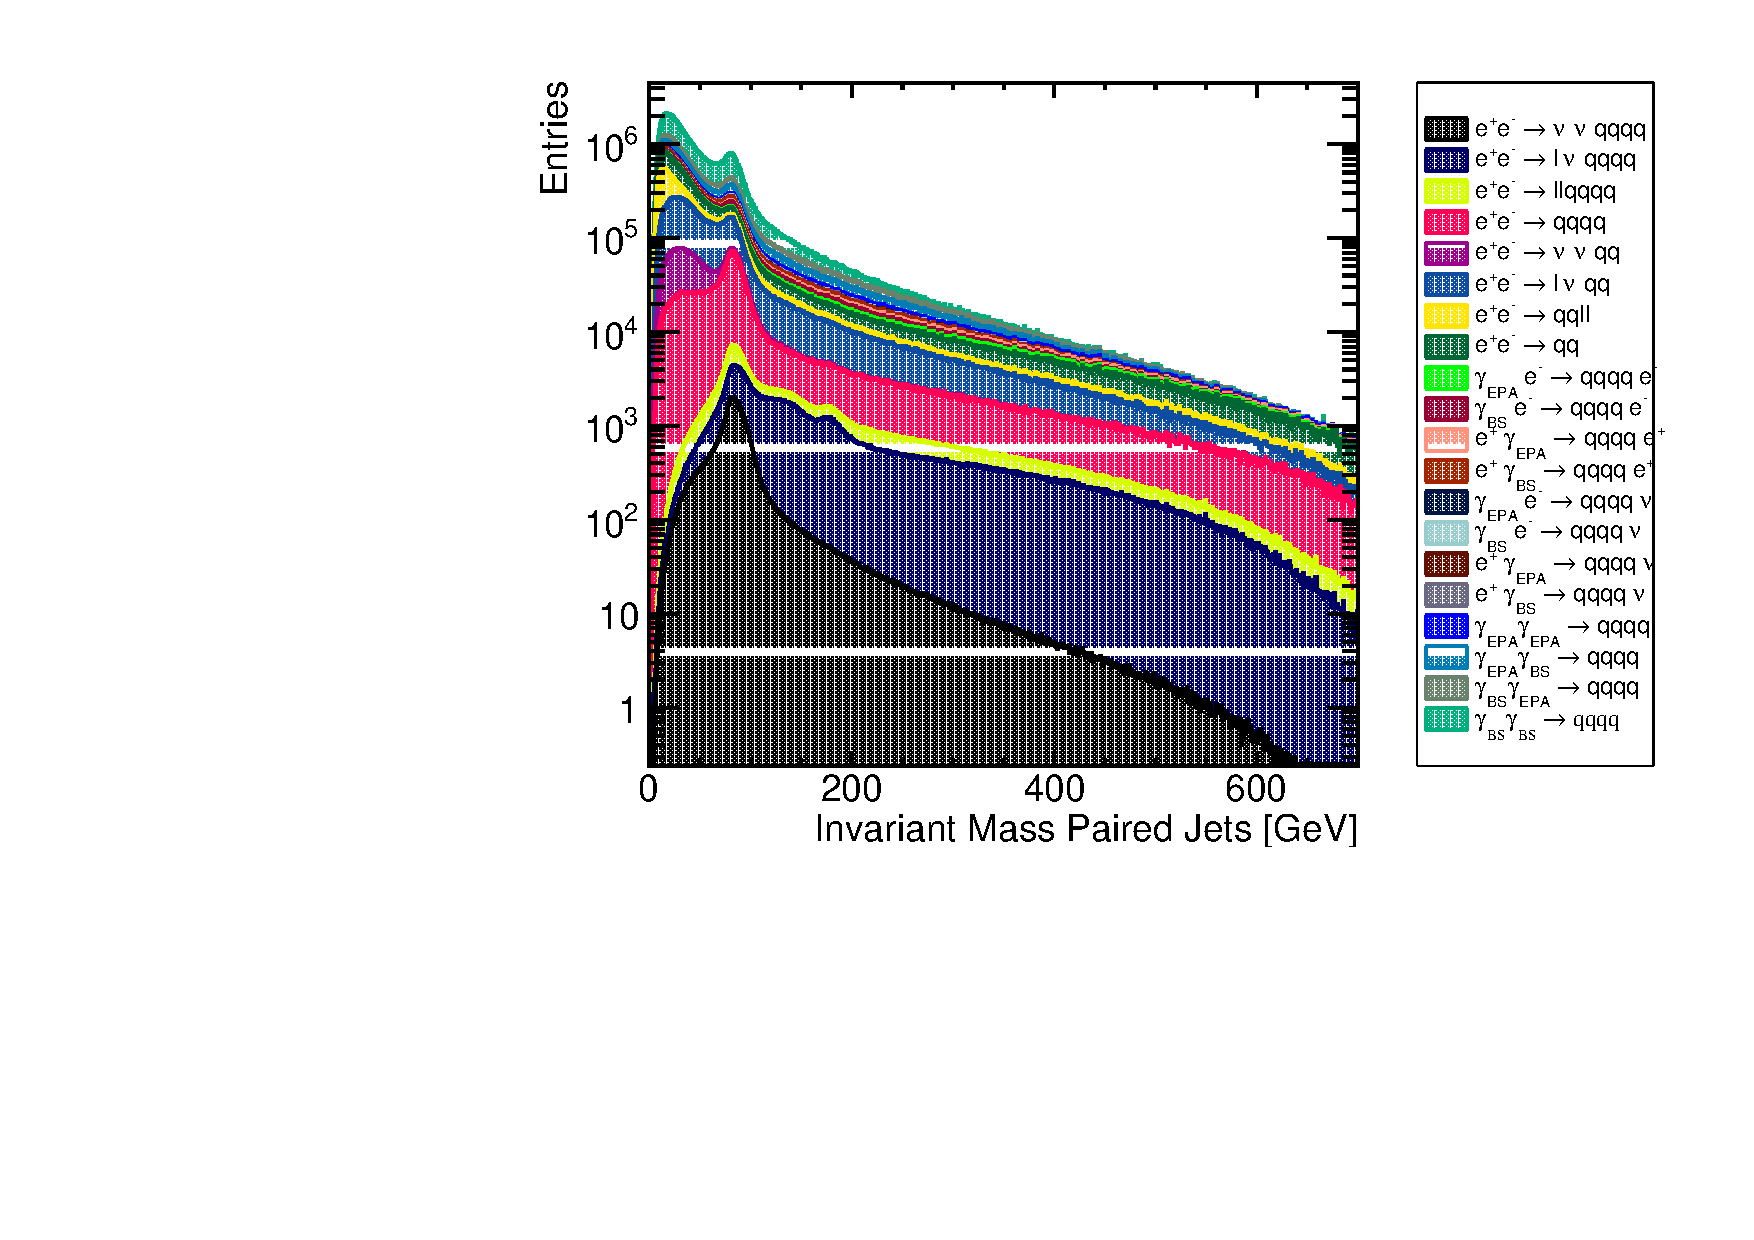
\includegraphics[width=0.5\textwidth]{PhysicsAnalysis/Plots/PostMVASelection/1400GeV/InvariantMassSynBosons_1400GeV_No_Cuts_StackPlot.pdf}}\hfill
\subfloat[Preselection cuts applied.]{\label{fig:nocutssynbosonmass1400GeVMVAimpact}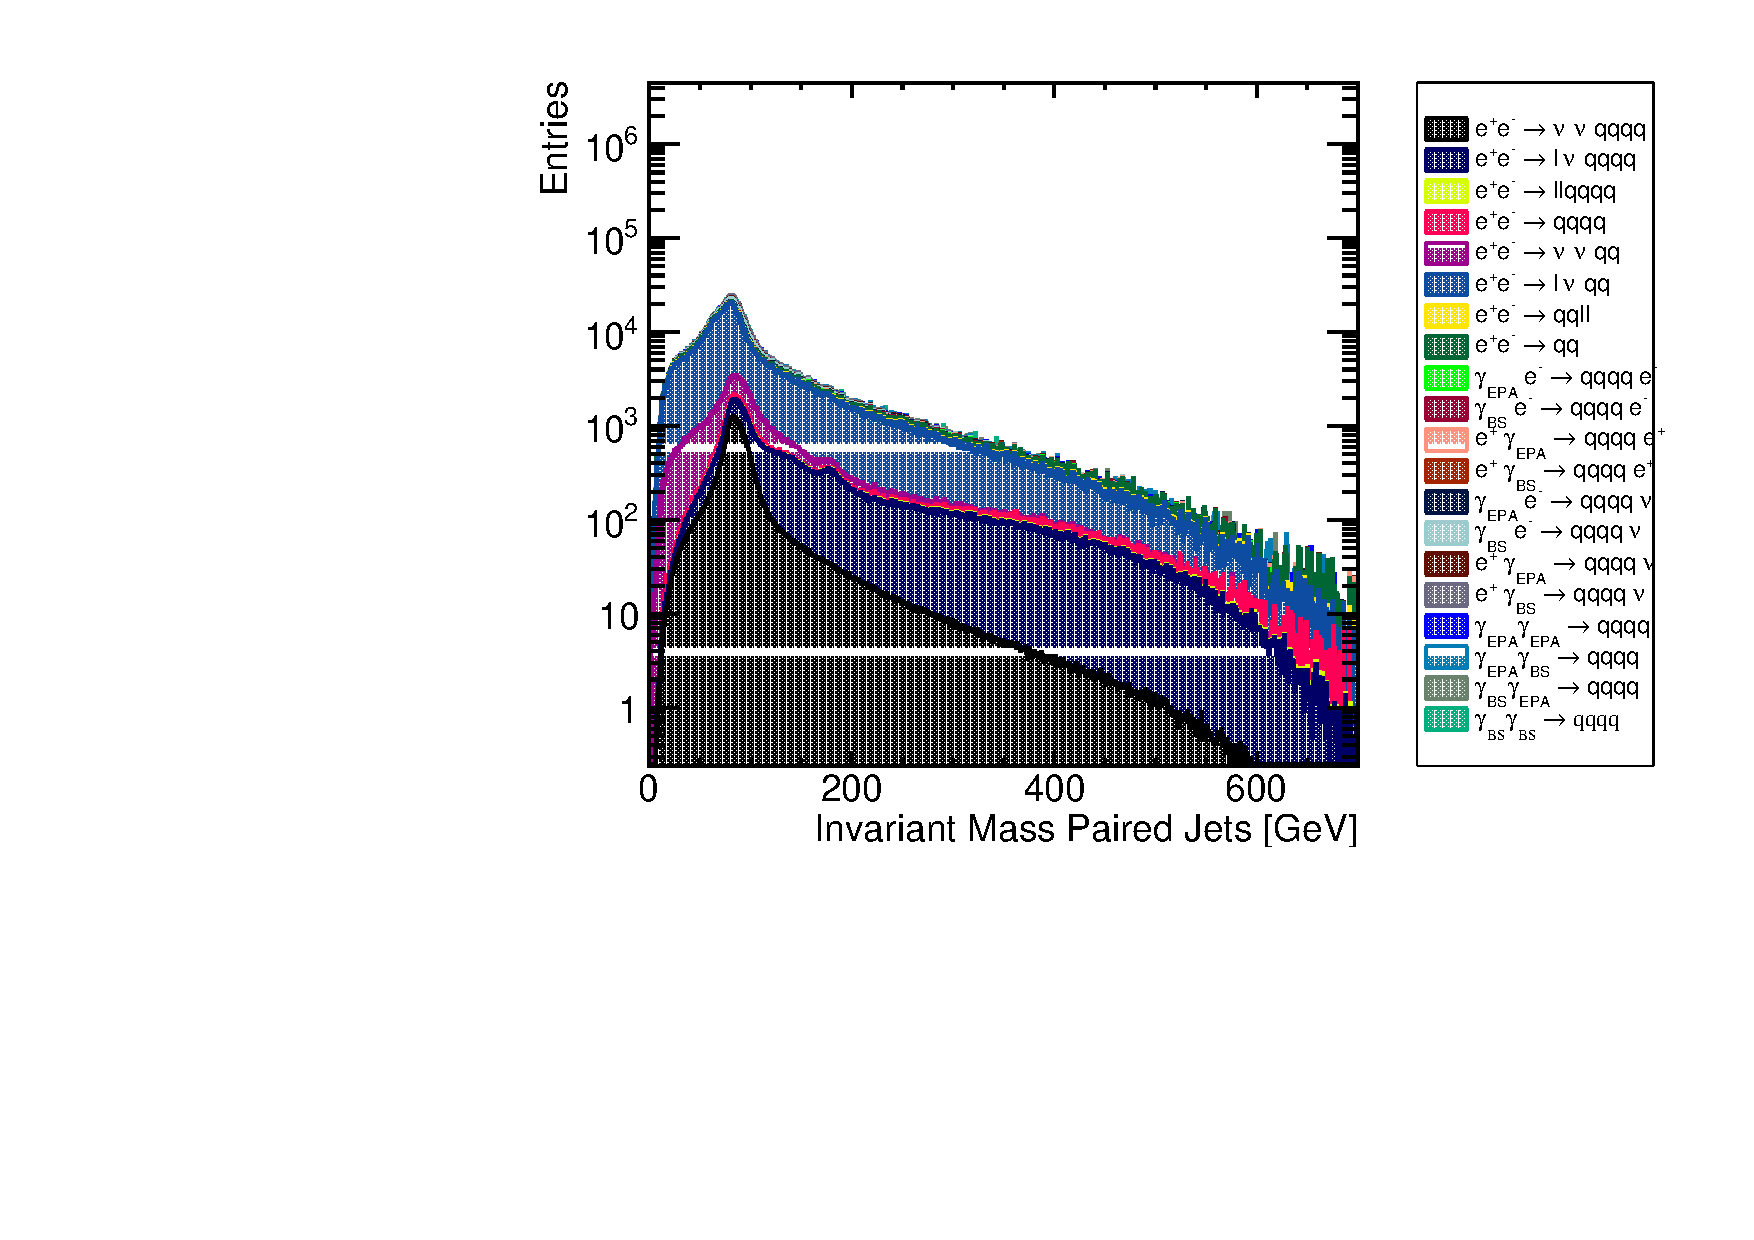
\includegraphics[width=0.5\textwidth]{PhysicsAnalysis/Plots/PostMVASelection/1400GeV/InvariantMassSynBosons_1400GeV_Pt_gt100GeV_MVis_gt200GeV_NIsoLep_eq0_Cuts_StackPlot.pdf}}
\subfloat[Preselection cuts and MVA applied.]{\label{fig:postmvasynbosonmass1400GeVMVAimpact}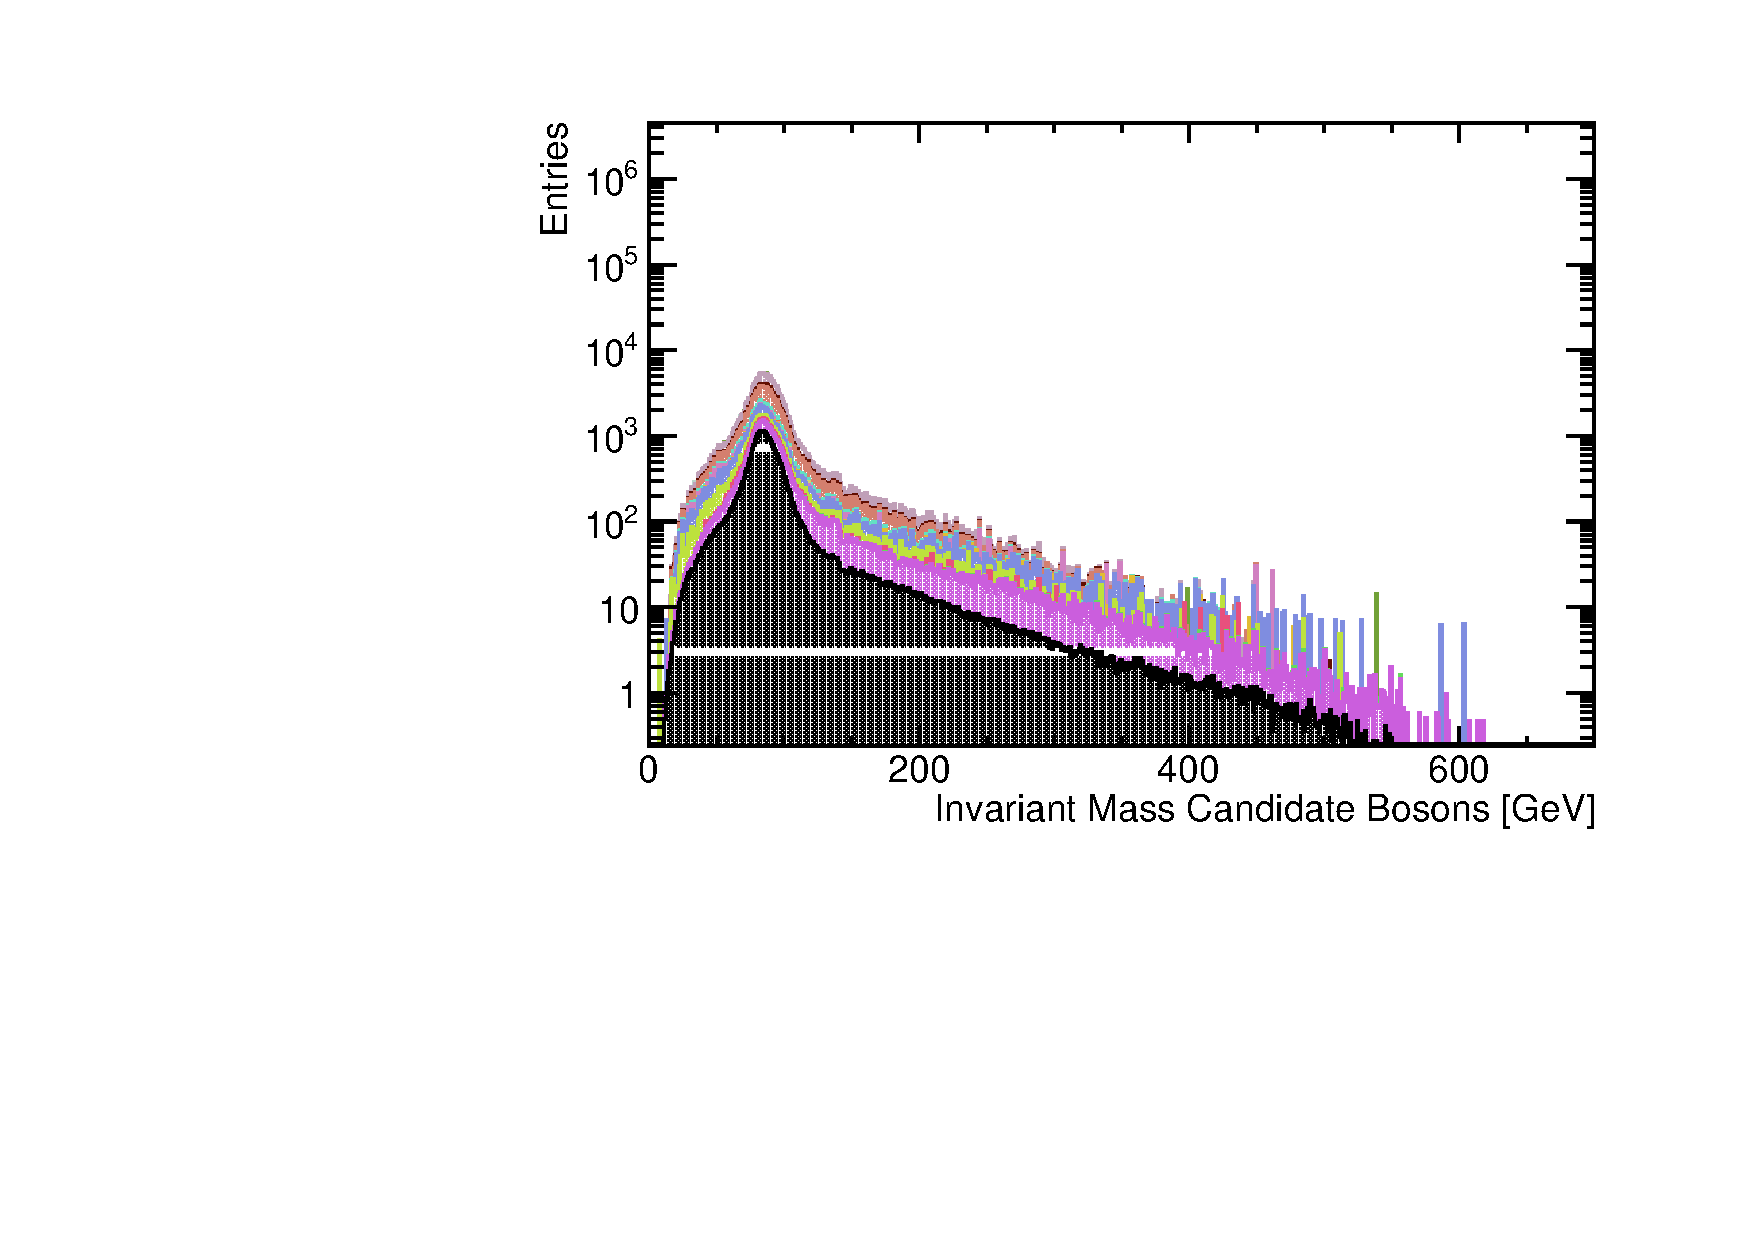
\includegraphics[width=0.5\textwidth]{PhysicsAnalysis/Plots/PostMVASelection/1400GeV/InvariantMassSynBosons_1400GeV_PostPreSelection_PostMVA_Cuts_StackPlot.pdf}} 
\caption[Impact of preselection and MVA on the reconstructed invariant mass of the bosons arising from jet pairing at 1.4 TeV.]{Impact of preselection and MVA on the reconstructed invariant mass of the bosons arising from jet pairing at 1.4 TeV.}
\label{fig:synbosonmass1400GeVMVAimpact}
\end{figure}

\begin{table}[h!]
\centering
\begin{tabular}{ l l l}
\hline
Final State & Raw Event Numbers & Post MVA Selection Numbers \\ 
\hline
$\text{e}^{+}\text{e}^{-} \rightarrow \nu{\nu}\text{qqqq}$ & 37,050 & 14,770 \\
$\text{e}^{+}\text{e}^{-} \rightarrow \text{l}\nu\text{qqqq}$ & 165,600 & 6,159 \\
$\text{e}^{+}\text{e}^{-} \rightarrow \text{llqqqq}$ & 93,150 & 80 \\
$\text{e}^{+}\text{e}^{-} \rightarrow \text{qqqq}$ & 1,868,000 & 1,264 \\
$\text{e}^{+}\text{e}^{-} \rightarrow \nu{\nu}\text{qq}$ & 1,181,000 & 3,286 \\
$\text{e}^{+}\text{e}^{-} \rightarrow \text{l}\nu\text{qq}$ & 6,464,000 & 6,262 \\
$\text{e}^{+}\text{e}^{-} \rightarrow \text{llqq}$ & 4,088,000 & 234 \\
$\text{e}^{+}\text{e}^{-} \rightarrow \text{qq}$ & 6,011,000 & 1,016 \\
$\gamma_{\text{EPA}}\text{e}^{-} \rightarrow \text{qqqq}\text{e}^{-}$ & 430,300 & 20 \\
$\gamma_{\text{BS}}\text{e}^{-} \rightarrow \text{qqqq}\text{e}^{-}$ & 1,306,000 & 42 \\
$\text{e}^{+}\gamma_{\text{EPA}} \rightarrow \text{qqqq}\text{e}^{+}$ & 430,300 & 19 \\
$\text{e}^{+}\gamma_{\text{BS}} \rightarrow \text{qqqq}\text{e}^{+}$ & 1,301,000 & 44 \\
$\gamma_{\text{EPA}}\text{e}^{-} \rightarrow \text{qqqq}\nu$ & 48,890 & 3,552 \\
$\gamma_{\text{BS}}\text{e}^{-} \rightarrow \text{qqqq}\nu$ & 154,000 & 18,540 \\
$\text{e}^{+}\gamma_{\text{EPA}} \rightarrow \text{qqqq}\nu$ & 48,890 & 3,652 \\
$\text{e}^{+}\gamma_{\text{BS}} \rightarrow \text{qqqq}\nu$ & 153,400 & 18,770 \\
$\gamma_{\text{EPA}}\gamma_{\text{EPA}} \rightarrow \text{qqqq}$ & 1,129,000 & 68 \\
$\gamma_{\text{EPA}}\gamma_{\text{BS}} \rightarrow \text{qqqq}$ & 4,539,000 & 55 \\
$\gamma_{\text{BS}}\gamma_{\text{EPA}} \rightarrow \text{qqqq}$ & 4,521,000 & 0 \\
$\gamma_{\text{BS}}\gamma_{\text{BS}} \rightarrow \text{qqqq}$ & 20,550,000 & 0 \\
\hline
\end{tabular}
\caption[Number of events passing the MVA selection at 1.4TeV.]{Number of events passing the MVA selection at 1.4TeV.  Event numbers are normalised to the correct luminosity for CLIC at 1.4 TeV.   The subscript EPA or BS for the incoming photons indicate whether the photon is generated from the equivalent photon approximation or beamstrahlung.}
\label{table:postmvanumbers1400GeV}
\end{table}

The summary of the selection procedure is given in table \ref{table:selectionsummary1400GeV}.

\begin{table}[h!]
\centering
\begin{tabular}{ l l l l}
\hline
Final State & $\epsilon_{\text{presel}}$ & $\epsilon_{\text{BDT}}$ & $N_{\text{BDT}}$ \\ 
\hline
$\text{e}^{+}\text{e}^{-} \rightarrow \nu{\nu}\text{qqqq}$ & 56.7\% & 39.9\% & 14,770 \\
$\text{e}^{+}\text{e}^{-} \rightarrow \text{l}\nu\text{qqqq}$ & 25.7\% & 3.7\% & 6,159 \\
$\text{e}^{+}\text{e}^{-} \rightarrow \nu{\nu}\text{qq}$ & 4.3\% & 0.3\% & 3,286 \\
$\text{e}^{+}\text{e}^{-} \rightarrow \text{l}\nu\text{qq}$ & 8.8\% & 0.1\% & 6,262 \\
$\gamma_{\text{EPA}}\text{e}^{-} \rightarrow \text{qqqq}\nu$ & 18.0\% & 7.3\% & 3,552 \\
$\gamma_{\text{BS}}\text{e}^{-} \rightarrow \text{qqqq}\nu$ & 23.2\% & 12.0\% & 18,540 \\
$\text{e}^{+}\gamma_{\text{EPA}} \rightarrow \text{qqqq}\nu$ & 18.2\% & 7.5\% & 3,652 \\
$\text{e}^{+}\gamma_{\text{BS}} \rightarrow \text{qqqq}\nu$ & 23.4\% & 12.2\% & 18,770 \\
\hline
\end{tabular}
\caption[Selection summary at 1.4TeV.]{Selection summary at 1.4TeV.   The subscript EPA or BS for the incoming photons indicate whether the photon is generated from the equivalent photon approximation or beamstrahlung.  Channels omitted from this table have less than 1,500 events in the post MVA selection.}
\label{table:selectionsummary1400GeV}
\end{table}

\subsection{Pre Selection - 3 TeV}

\begin{table}[h!]
\centering
\begin{tabular}{ l l l l l}
\hline
Final State & Raw Event  & $p_{T}$ > 100 GeV & $p_{T}$ > 100 GeV \& & $p_{T}$ > 100 GeV \& \\ 
& Numbers & & $M_{\text{Vis}}$ > 200 GeV & $M_{\text{Vis}}$ > 200 GeV \&\\ 
& & & & $N_{\text{Isolated Leptons}}$ = 0\\ 
\hline
$\text{e}^{+}\text{e}^{-} \rightarrow \nu{\nu}\text{qqqq}$ & 143,000 & 106,600 & 99,390 & 99,130 \\ 
$\text{e}^{+}\text{e}^{-} \rightarrow \text{l}\nu\text{qqqq}$ & 213,200 & 129,800 & 127,300 & 82,880 \\
$\text{e}^{+}\text{e}^{-} \rightarrow \text{llqqqq}$ &338,600 & 32,750 & 31,010 & 23,550 \\
$\text{e}^{+}\text{e}^{-} \rightarrow \text{qqqq}$ & 1,093,000 & 40,180 & 37,360 & 37,300 \\ 
$\text{e}^{+}\text{e}^{-} \rightarrow \nu{\nu}\text{qq}$ & 2,634,000 & 1,333,000 & 380,100 & 379,500 \\
$\text{e}^{+}\text{e}^{-} \rightarrow \text{l}\nu\text{qq}$ & 11,120,000 & 4,240,000 & 2,479,000 & 1,836,000 \\
$\text{e}^{+}\text{e}^{-} \rightarrow \text{llqq}$ & 6,639,000 & 131,400 & 84,980 & 54,780 \\ 
$\text{e}^{+}\text{e}^{-} \rightarrow \text{qq}$ &5,897,000 & 79,440 & 66,790 & 66,730 \\
$\gamma_{\text{EPA}}\text{e}^{-} \rightarrow \text{qqqq}\text{e}^{-}$ & 575,600 & 57,920 & 54,640 & 34,480 \\ 
$\gamma_{\text{BS}}\text{e}^{-} \rightarrow \text{qqqq}\text{e}^{-}$ & 2,004,000 & 99,930 & 90,750 & 83,440 \\
$\text{e}^{+}\gamma_{\text{EPA}} \rightarrow \text{qqqq}\text{e}^{+}$ & 575,600 & 57,990 & 54,290 & 34,190 \\
$\text{e}^{+}\gamma_{\text{BS}} \rightarrow \text{qqqq}\text{e}^{+}$ & 2,002,000 & 100,300 & 90,830 & 83,960 \\   
$\gamma_{\text{EPA}}\text{e}^{-} \rightarrow \text{qqqq}\nu$ & 108,400 & 63,780 & 60,660 & 46,380 \\
$\gamma_{\text{BS}}\text{e}^{-} \rightarrow \text{qqqq}\nu$ & 414,700 & 233,800 & 215,600 & 213,600 \\
$\text{e}^{+}\gamma_{\text{EPA}} \rightarrow \text{qqqq}\nu$ & 108,400 & 64,230 & 61,130 & 46,720 \\ 
$\text{e}^{+}\gamma_{\text{BS}} \rightarrow \text{qqqq}\nu$ & 414,400 & 236,400 & 219,000 & 217,000 \\
$\gamma_{\text{EPA}}\gamma_{\text{EPA}} \rightarrow \text{qqqq}$ & 805,400 & 54,010 & 48,720 & 37,730 \\ 
$\gamma_{\text{EPA}}\gamma_{\text{BS}} \rightarrow \text{qqqq}$ & 3,828,000 & 150,800 & 131,600 & 114,500 \\ 
$\gamma_{\text{BS}}\gamma_{\text{EPA}} \rightarrow \text{qqqq}$ & 3,825,000 & 150,600 & 133,600 & 116,900 \\ 
$\gamma_{\text{BS}}\gamma_{\text{BS}} \rightarrow \text{qqqq}$ & 18,010,000 & 123,500 & 115,400 & 105,000 \\
\hline
\end{tabular}
\caption[Number of events passing the various cuts applied in the preselection at 3 TeV.]{Number of events passing the various cuts applied in the preselection at 3 TeV.  Event numbers are normalised to the correct luminosity for CLIC at 3 TeV.  $p_{T}$ is the transverse momentum of the event,  $M_{\text{Vis}}$ is the visible mass and $N_{\text{Isolated Leptons}}$ is the number of isolated leptons in the event.  In the above table q $\in$ u, $\bar{\text{u}}$, d, $\bar{\text{d}}$, s, $\bar{\text{s}}$, c, $\bar{\text{c}}$, b or $\bar{\text{b}}$ while l $\in$ $\text{e}^{\pm}$, $\mu^{\pm}$ or $\tau^{\pm}$ and $\nu$ $\in$ $\nu_{e}$, $\nu_{\mu}$ and $\nu_{\tau}$.  The subscript EPA or BS for the incoming photons indicate whether the photon is generated from the equivalent photon approximation or beamstrahlung.}
\label{table:preselectionnumbers3000GeV}
\end{table}

\begin{figure}
\centering
\subfloat[Transverse momentum of system.]{\label{fig:preselection3000_1}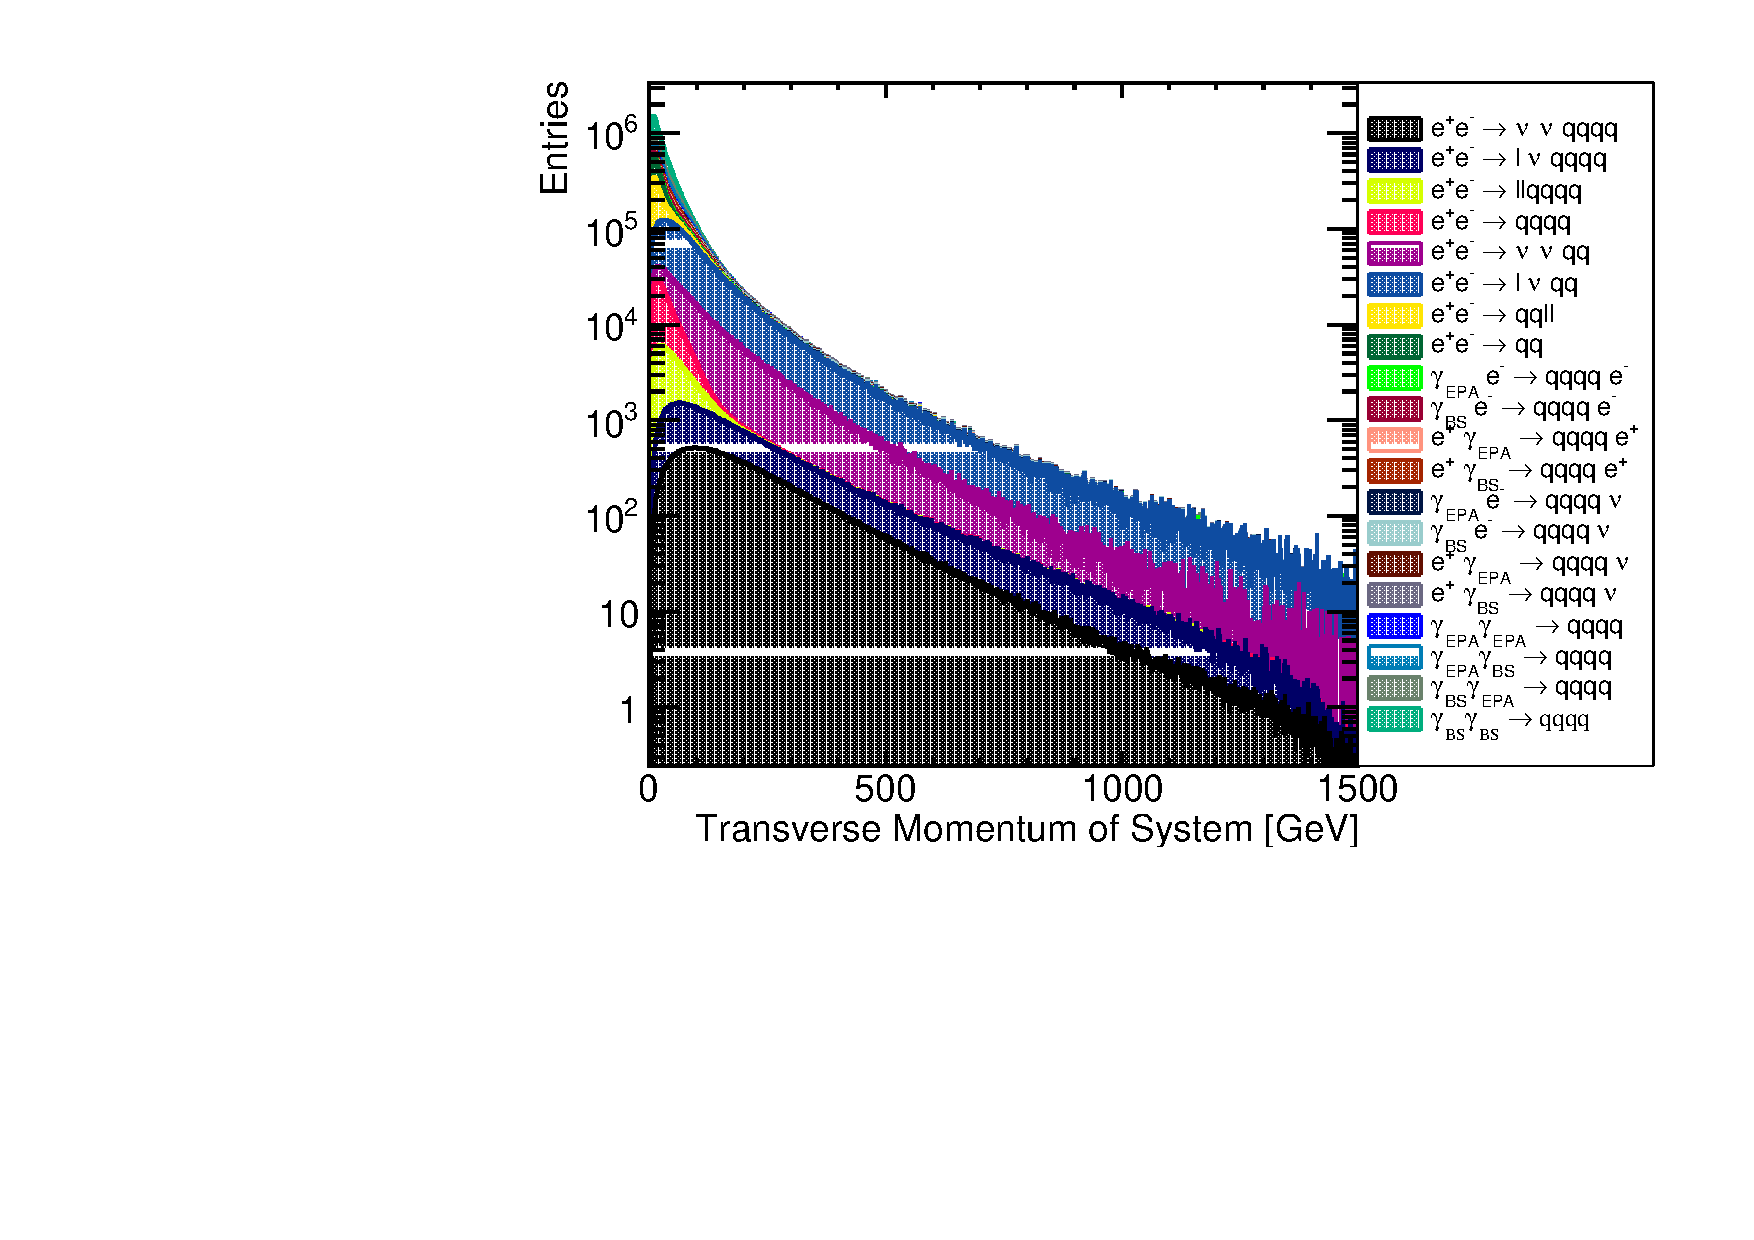
\includegraphics[width=0.5\textwidth]{PhysicsAnalysis/Plots/PreSelection/3000GeV/TransverseMomentum.pdf}}\hfill
\subfloat[Invariant mass of the visible system.]{\label{fig:preselection3000_2}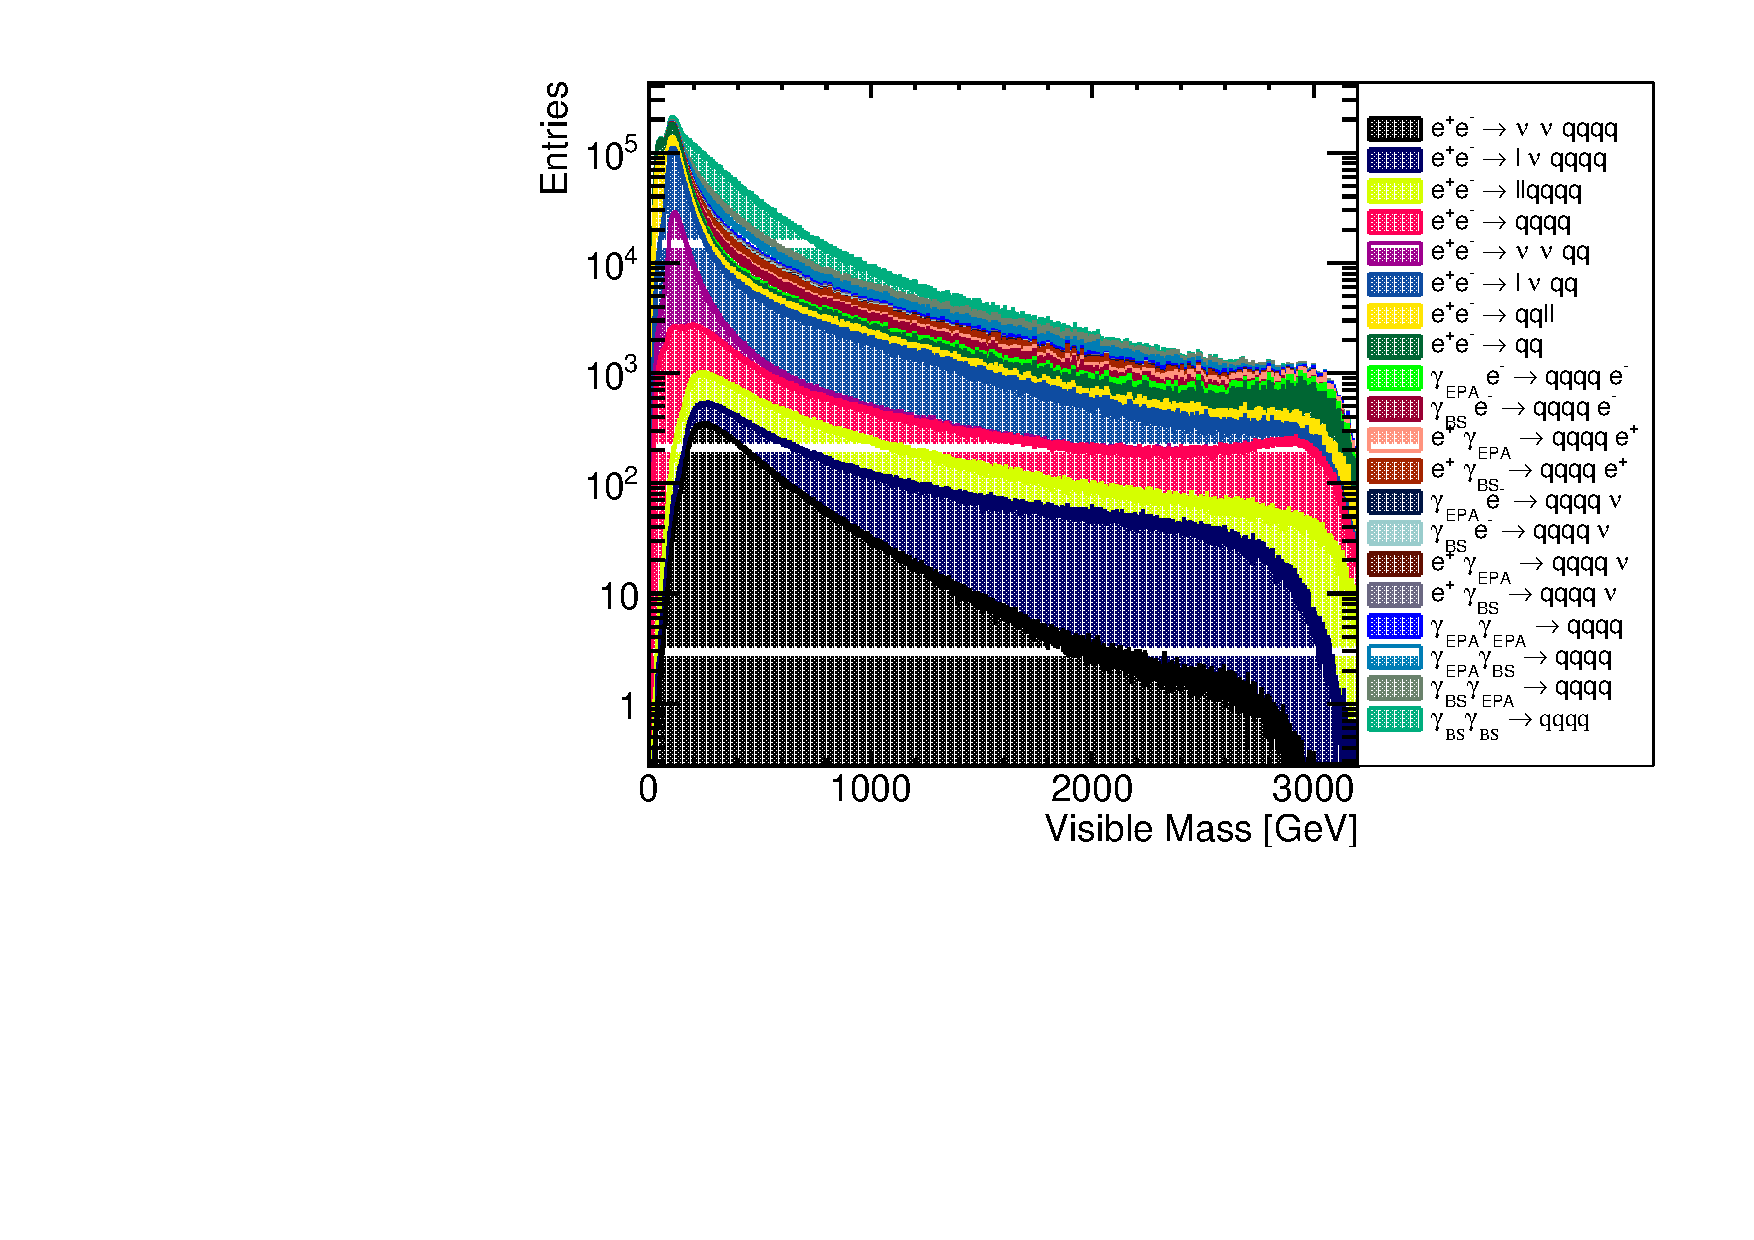
\includegraphics[width=0.5\textwidth]{PhysicsAnalysis/Plots/PreSelection/3000GeV/InvariantMassSystem.pdf}}
\subfloat[Number of isolated leptons.]{\label{fig:preselection3000_3}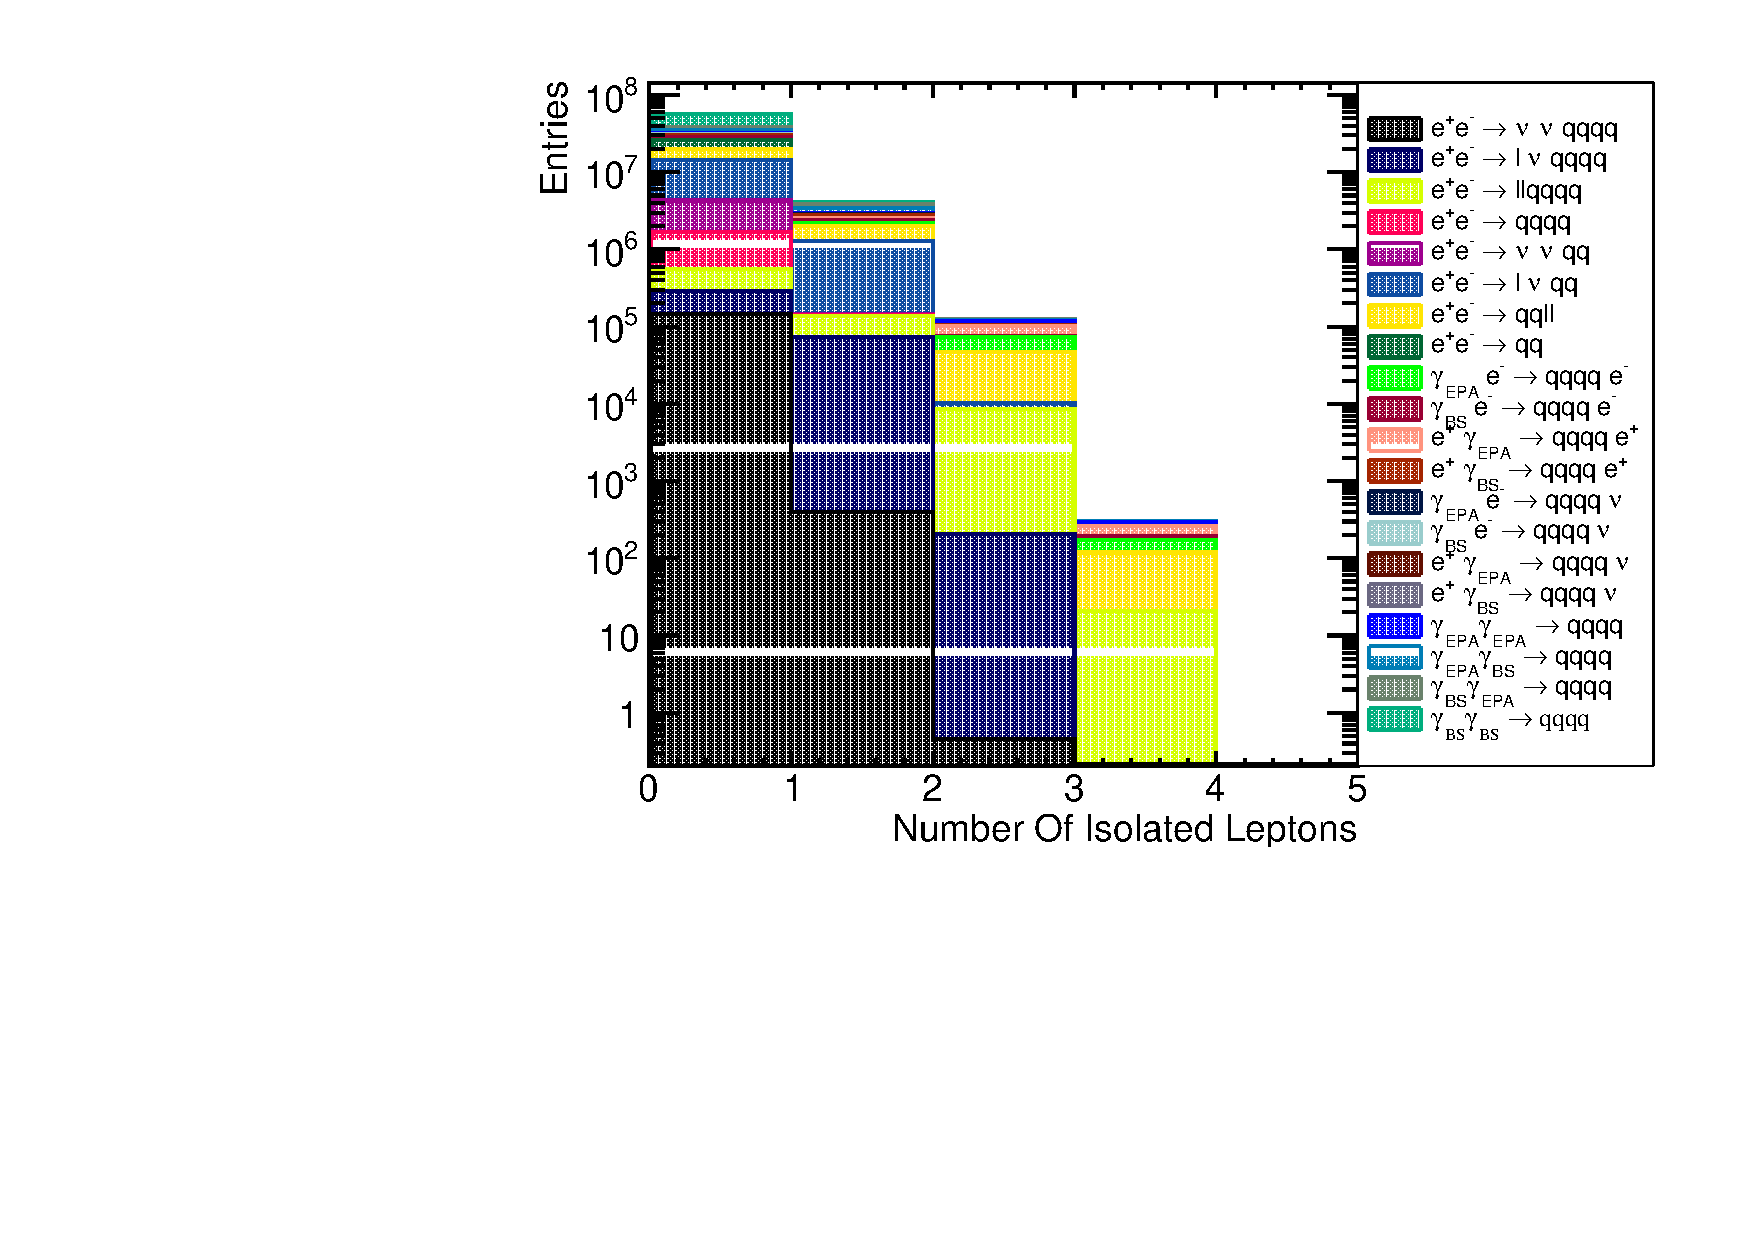
\includegraphics[width=0.5\textwidth]{PhysicsAnalysis/Plots/PreSelection/3000GeV/NumberOfIsolatedLeptons.pdf}}
\caption[Distribution of variables cut on in the preselection at 3 TeV.]{Distribution of variables cut on in the preselection at 3 TeV.}
\label{fig:preselection3000}
\end{figure}

\subsection{MVA - 3 TeV}

\begin{table}[h!]
\centering
\begin{tabular}{ l l l}
\hline
Final State & Raw Event Numbers & Post MVA Selection Numbers \\ 
\hline
$\text{e}^{+}\text{e}^{-} \rightarrow \nu{\nu}\text{qqqq}$ & 143,000 & 64,750 \\
$\text{e}^{+}\text{e}^{-} \rightarrow \text{l}\nu\text{qqqq}$ & 213,200 & 23,310 \\
$\text{e}^{+}\text{e}^{-} \rightarrow \text{llqqqq}$ & 338,600 & 2,409 \\
$\text{e}^{+}\text{e}^{-} \rightarrow \text{qqqq}$ & 1,093,000 & 3,069 \\
$\text{e}^{+}\text{e}^{-} \rightarrow \nu{\nu}\text{qq}$ & 2,634,000 & 19,040 \\
$\text{e}^{+}\text{e}^{-} \rightarrow \text{l}\nu\text{qq}$ & 11,120,000 & 27,910 \\
$\text{e}^{+}\text{e}^{-} \rightarrow \text{llqq}$ & 6,639,000 & 786 \\
$\text{e}^{+}\text{e}^{-} \rightarrow \text{qq}$ & 5,897,000 & 1,335 \\
$\gamma_{\text{EPA}}\text{e}^{-} \rightarrow \text{qqqq}\text{e}^{-}$ & 575,600 & 2,860 \\
$\gamma_{\text{BS}}\text{e}^{-} \rightarrow \text{qqqq}\text{e}^{-}$ & 2,004,000 & 8,352 \\
$\text{e}^{+}\gamma_{\text{EPA}} \rightarrow \text{qqqq}\text{e}^{+}$ & 575,600 & 3,063 \\
$\text{e}^{+}\gamma_{\text{BS}} \rightarrow \text{qqqq}\text{e}^{+}$ & 2,002,000 & 8,090 \\
$\gamma_{\text{EPA}}\text{e}^{-} \rightarrow \text{qqqq}\nu$ & 108,400 & 17,950 \\
$\gamma_{\text{BS}}\text{e}^{-} \rightarrow \text{qqqq}\nu$ & 414,700 & 108,000 \\
$\text{e}^{+}\gamma_{\text{EPA}} \rightarrow \text{qqqq}\nu$ & 108,400 & 17,980 \\
$\text{e}^{+}\gamma_{\text{BS}} \rightarrow \text{qqqq}\nu$ & 414,400 & 109,700 \\
$\gamma_{\text{EPA}}\gamma_{\text{EPA}} \rightarrow \text{qqqq}$ & 805,400 & 3,058 \\
$\gamma_{\text{EPA}}\gamma_{\text{BS}} \rightarrow \text{qqqq}$ & 3,828,000 & 9,812 \\
$\gamma_{\text{BS}}\gamma_{\text{EPA}} \rightarrow \text{qqqq}$ & 3,825,000 & 8,880 \\
$\gamma_{\text{BS}}\gamma_{\text{BS}} \rightarrow \text{qqqq}$ & 18,010,000 & 2,213 \\
\hline
\end{tabular}
\caption[Number of events passing the MVA selection at 3 TeV.]{Number of events passing the MVA selection at 3 TeV.  Event numbers are normalised to the correct luminosity for CLIC at 3 TeV.   The subscript EPA or BS for the incoming photons indicate whether the photon is generated from the equivalent photon approximation or beamstrahlung.}
\label{table:postmvanumbers3000GeV}
\end{table}

\begin{table}[h!]
\centering
\begin{tabular}{ l l l l}
\hline
Final State & $\epsilon_{\text{presel}}$ & $\epsilon_{\text{BDT}}$ & $N_{\text{BDT}}$ \\ 
\hline
$\text{e}^{+}\text{e}^{-} \rightarrow \nu{\nu}\text{qqqq}$ & 69.4\% & 45.3\% & 64.750 \\
$\text{e}^{+}\text{e}^{-} \rightarrow \text{l}\nu\text{qqqq}$ & 38.9\% & 10.9\% & 23,310 \\
$\text{e}^{+}\text{e}^{-} \rightarrow \nu{\nu}\text{qq}$ & 14.4\% & 0.7\% & 19,040 \\
$\text{e}^{+}\text{e}^{-} \rightarrow \text{l}\nu\text{qq}$ & 16.5\% & 0.3\% & 27,910 \\
$\gamma_{\text{BS}}\text{e}^{-} \rightarrow \text{qqqq}\text{e}^{-}$ & 4.1\% & 0.4\% & 8,352 \\
$\text{e}^{+}\gamma_{\text{BS}} \rightarrow \text{qqqq}\text{e}^{+}$ & 4.2\% & 0.4\% & 8,090 \\
$\gamma_{\text{EPA}}\text{e}^{-} \rightarrow \text{qqqq}\nu$ & 42.8\% & 16.6\% & 17,950 \\
$\gamma_{\text{BS}}\text{e}^{-} \rightarrow \text{qqqq}\nu$ & 51.6\% & 26.0\% & 108,000 \\
$\text{e}^{+}\gamma_{\text{EPA}} \rightarrow \text{qqqq}\nu$ & 43.1\% & 16.6\% & 17,980 \\
$\text{e}^{+}\gamma_{\text{BS}} \rightarrow \text{qqqq}\nu$ & 52.3\% & 26.5\% & 109,700 \\
$\gamma_{\text{EPA}}\gamma_{\text{BS}} \rightarrow \text{qqqq}$ & 3.0\% & 0.3\% & 9,812 \\
$\gamma_{\text{BS}}\gamma_{\text{EPA}} \rightarrow \text{qqqq}$ & 3.1\% & 0.2\% & 8,880 \\
\hline
\end{tabular}
\caption[Selection summary at 3 TeV.]{Selection summary at 3 TeV.   The subscript EPA or BS for the incoming photons indicate whether the photon is generated from the equivalent photon approximation or beamstrahlung.  Channels omitted from this table have less than 6,000 events in the post MVA selection.}
\label{table:selectionsummary3000GeV}
\end{table}

\section{Results}
\subsection{1.4 TeV}
The sensitivity of the CLIC experiment to the anomalous gauge couplings $\alpha_{4}$ and $\alpha_{5}$ at 1.4 TeV is shown in figure \ref{fig:finalresult1400GeV}.  This result shows the sensitivity after the application of preselection and MVA described in sections \ref{sec:preselection1400GeV} and \ref{sec:mva1400GeV} purposed to remove the included background channels, described in section \ref{sec:eventgenerationandbackgrounds}.  These contours yield the one $\sigma$ confidence limit on the measurement of $\alpha_{4}$ to the range -0.00831, 0.0130 and similarly for the measurement of $\alpha_{5}$ the range is -0.00606, 0.00904.

\begin{figure}
\centering
\subfloat[$\chi^{2}$ sensitivity contours in $\alpha_{4}$ and $\alpha_{5}$ space.]{\label{fig:finalresult1400GeV}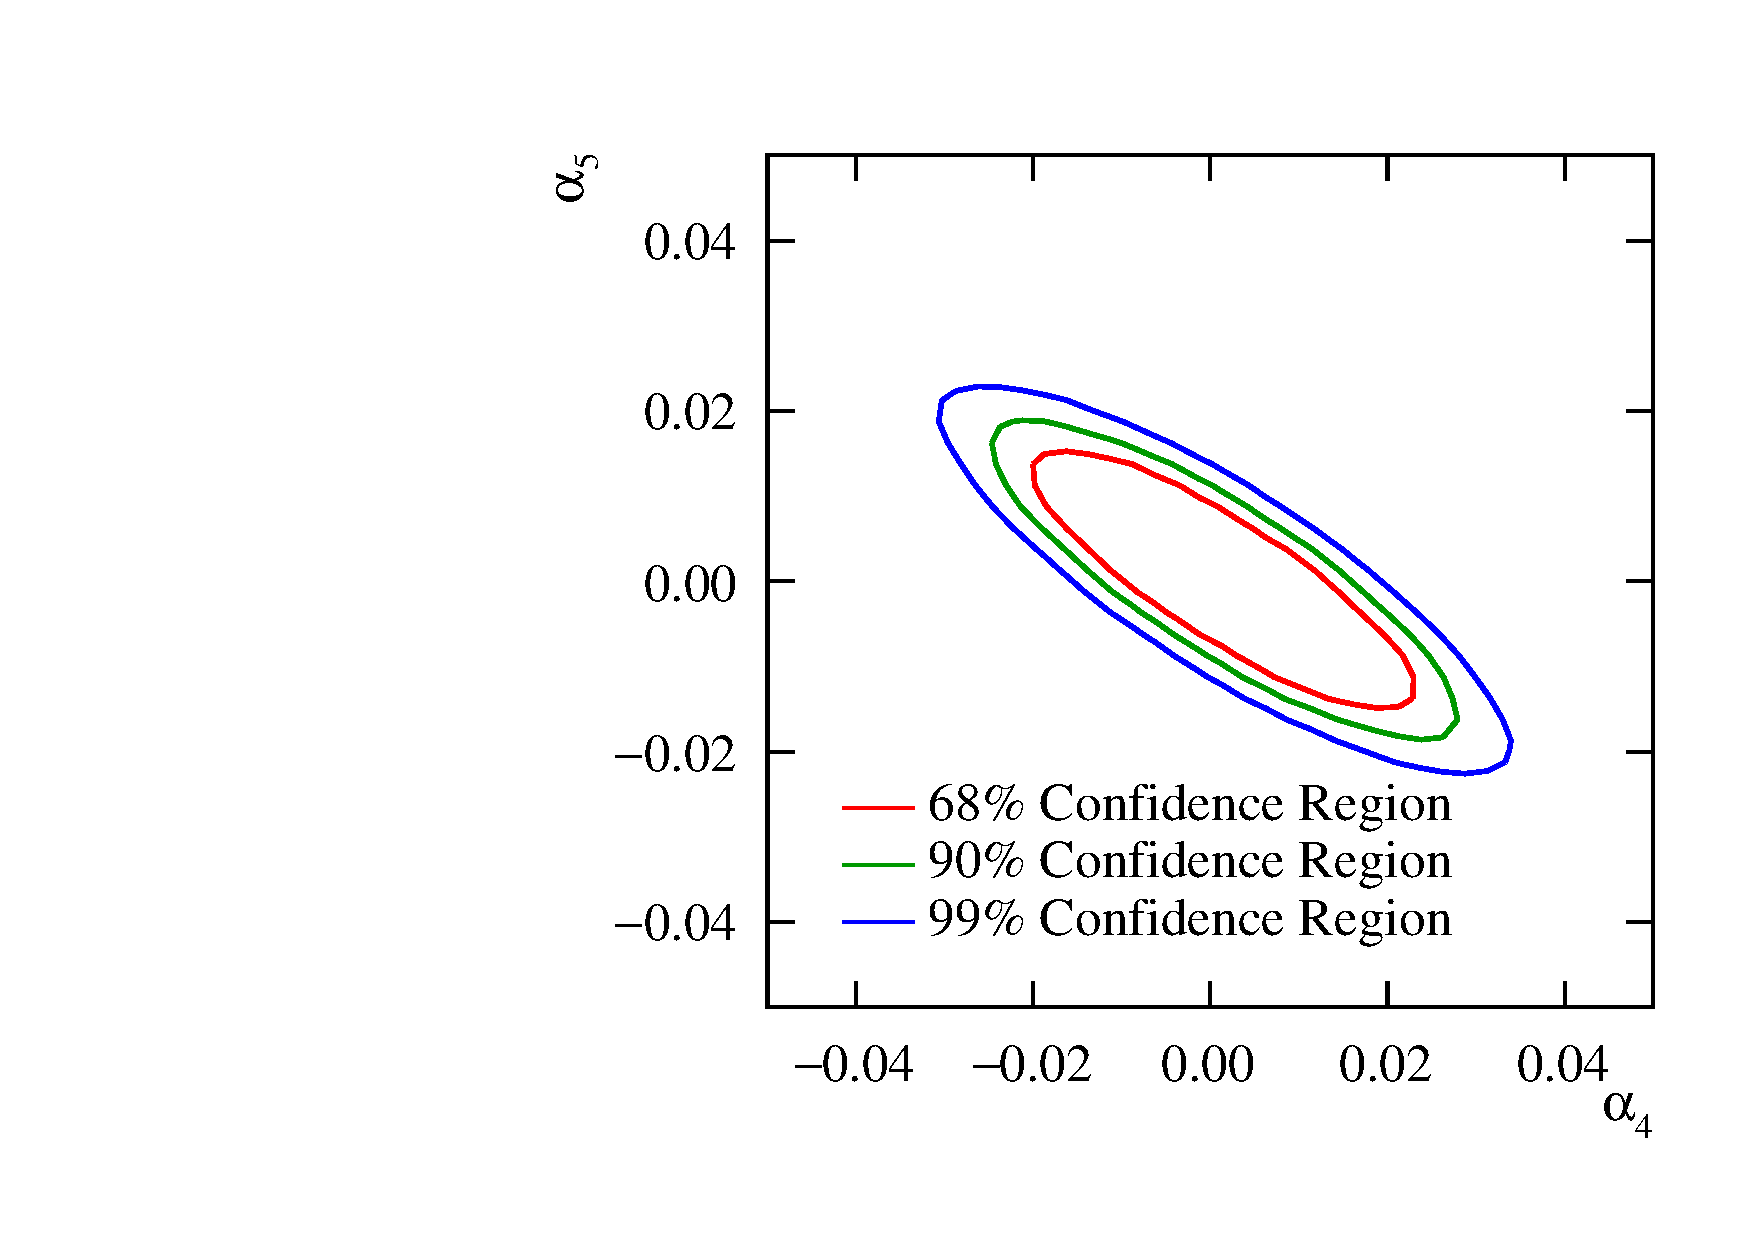
\includegraphics[width=0.5\textwidth]{PhysicsAnalysis/Plots/FinalResult/1400GeV/Final.pdf}}\hfill
\subfloat[$\chi^{2}$ as a function of $\alpha_{4}$ assuming $\alpha_{5} = 0$.]{\label{fig:a4finalresult1400GeV}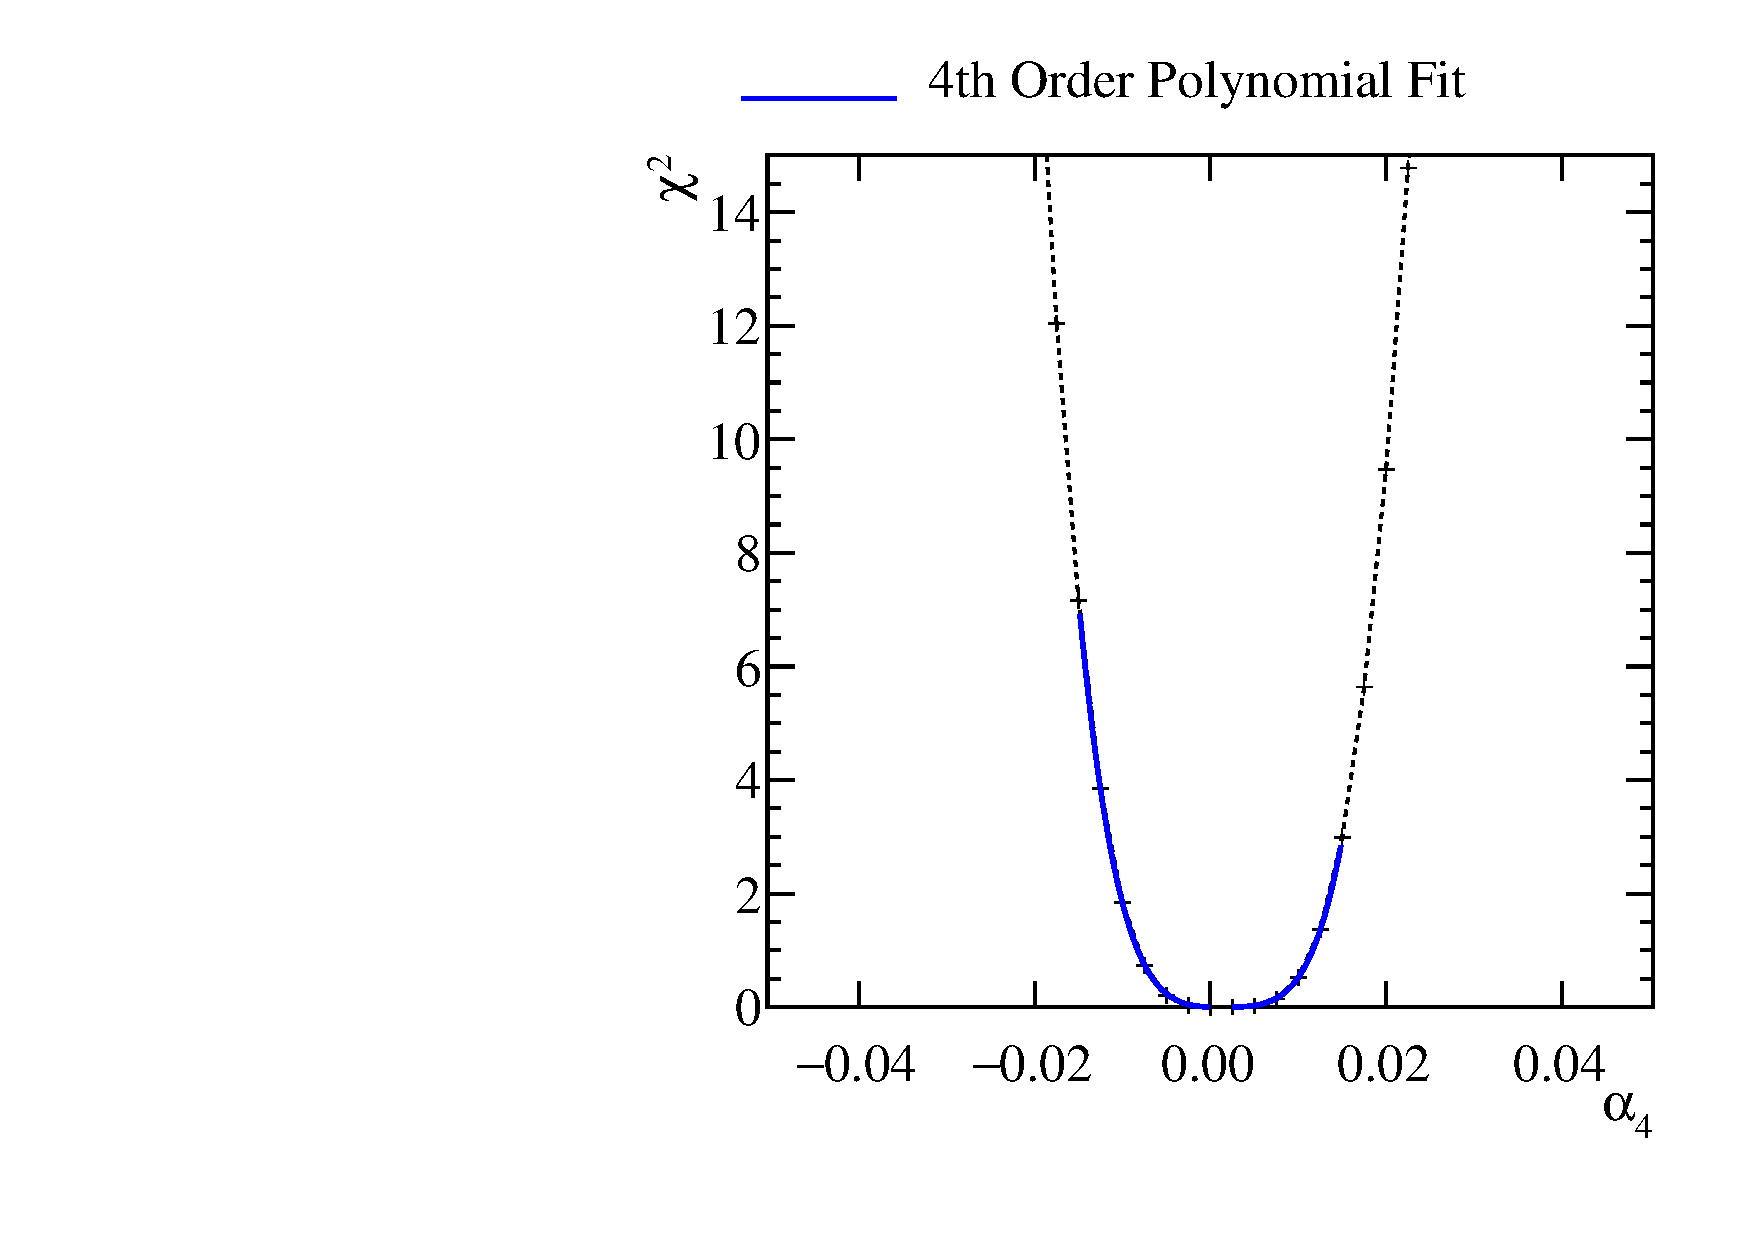
\includegraphics[width=0.5\textwidth]{PhysicsAnalysis/Plots/FinalResult/1400GeV/Final_alpha4.pdf}}
\subfloat[$\chi^{2}$ as a function of $\alpha_{5}$ assuming $\alpha_{4} = 0$.]{\label{fig:a5finalresult1400GeV}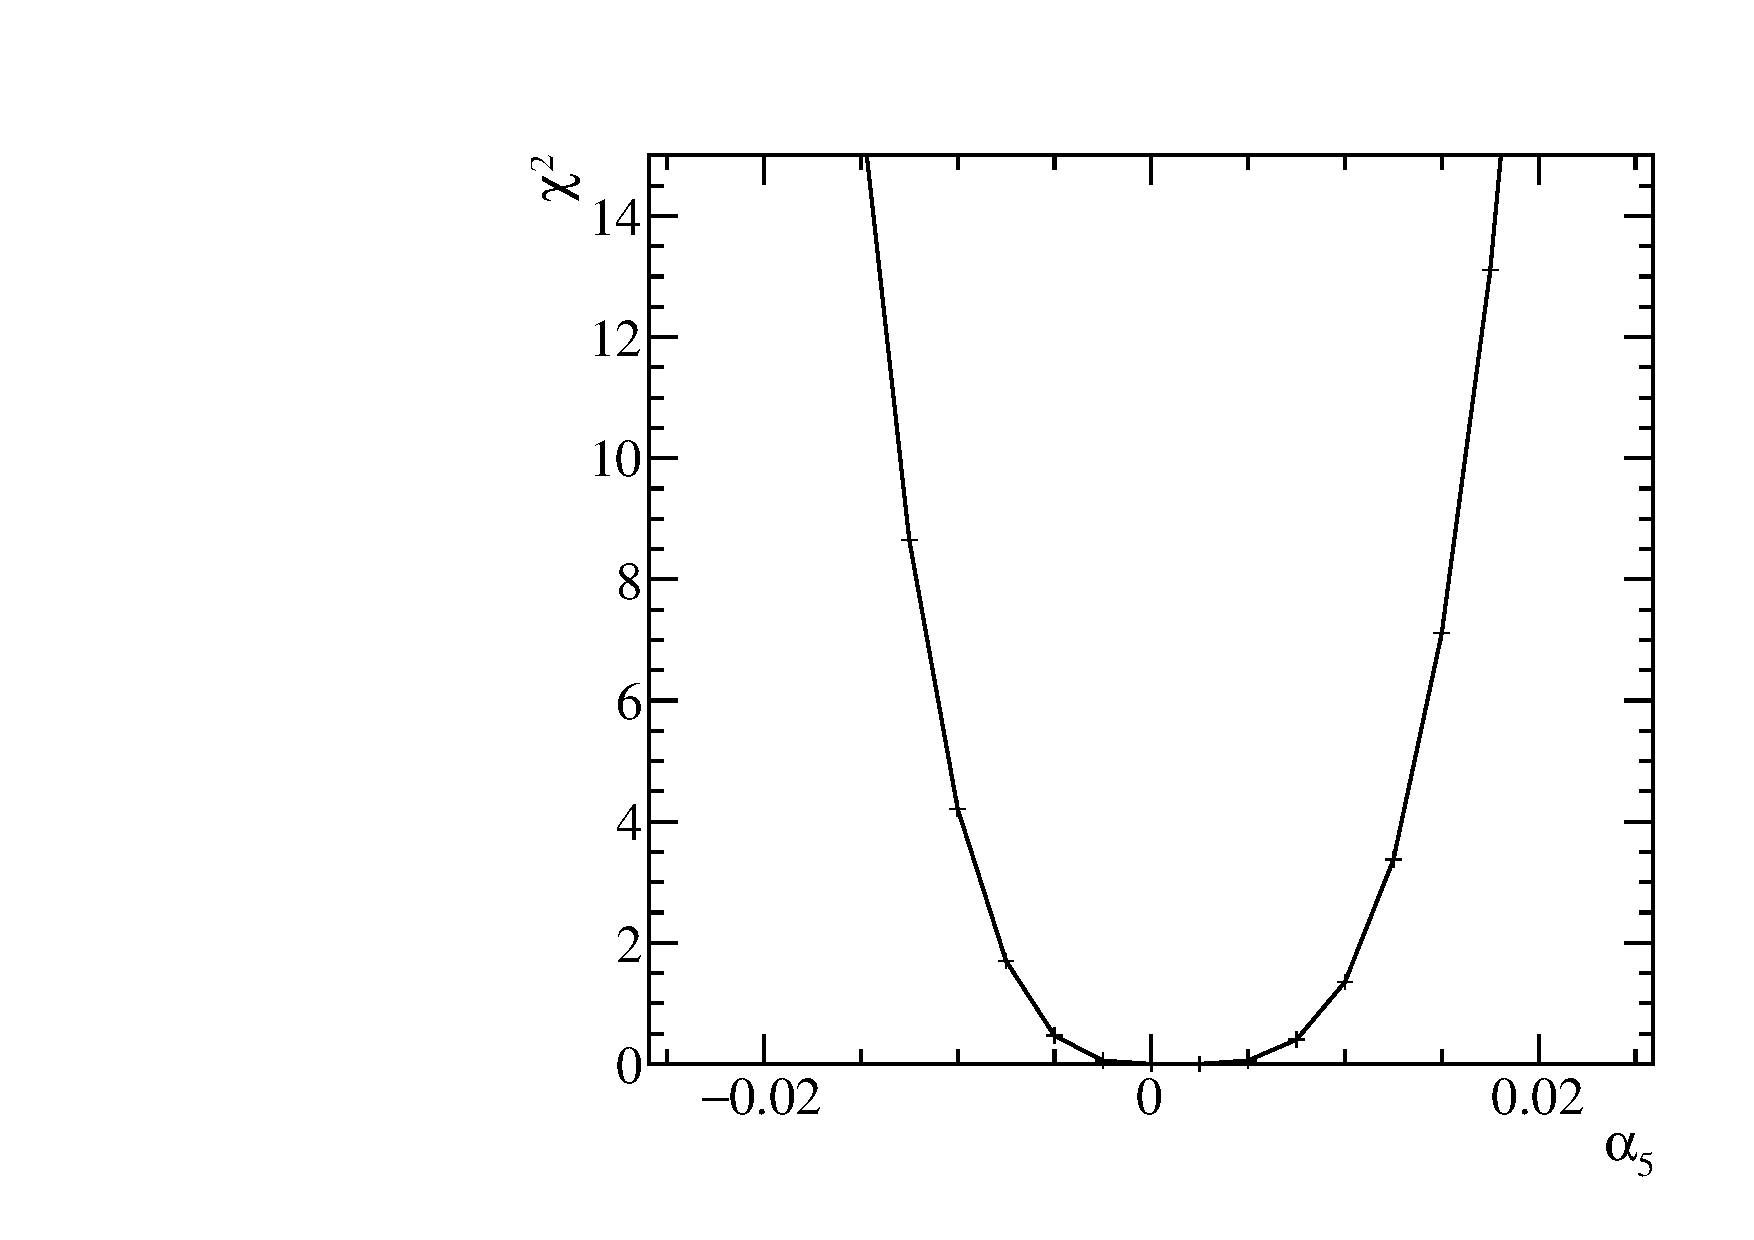
\includegraphics[width=0.5\textwidth]{PhysicsAnalysis/Plots/FinalResult/1400GeV/Final_alpha5.pdf}}
\caption[$\chi^{2}$ sensitivity distributions at 1.4 TeV arising from a fit to $\text{cos}\theta^{*}_{\text{Jets}}$.  Results include the effect of backgrounds after the application of preselection and MVA.]{$\chi^{2}$ sensitivity distributions at 1.4 TeV arising from a fit to $\text{cos}\theta^{*}_{\text{Jets}}$.  Results include the effect of backgrounds after the application of preselection and MVA.}
\label{fig:allfinalresult1400GeV}
\end{figure}

\iffalse
$\text{e}^{+}\text{e}^{-} \rightarrow \nu{\nu}\text{qqqq}$
$\text{e}^{+}\text{e}^{-} \rightarrow \text{l}\nu\text{qqqq}$
$\text{e}^{+}\text{e}^{-} \rightarrow \text{llqqqq}$
$\text{e}^{+}\text{e}^{-} \rightarrow \text{qqqq}$
$\text{e}^{+}\text{e}^{-} \rightarrow \nu{\nu}\text{qq}$
$\text{e}^{+}\text{e}^{-} \rightarrow \text{l}\nu\text{qq}$
$\text{e}^{+}\text{e}^{-} \rightarrow \text{llqq}$
$\text{e}^{+}\text{e}^{-} \rightarrow \text{qq}$
$\gamma_{\text{EPA}}\text{e}^{-} \rightarrow \text{qqqq}\text{e}^{-}$
$\gamma_{\text{BS}}\text{e}^{-} \rightarrow \text{qqqq}\text{e}^{-}$
$\text{e}^{+}\gamma_{\text{EPA}} \rightarrow \text{qqqq}\text{e}^{+}$
$\text{e}^{+}\gamma_{\text{BS}} \rightarrow \text{qqqq}\text{e}^{+}$
$\gamma_{\text{EPA}}\text{e}^{-} \rightarrow \text{qqqq}\nu$
$\gamma_{\text{BS}}\text{e}^{-} \rightarrow \text{qqqq}\nu$
$\text{e}^{+}\gamma_{\text{EPA}} \rightarrow \text{qqqq}\nu$
$\text{e}^{+}\gamma_{\text{BS}} \rightarrow \text{qqqq}\nu$
$\gamma_{\text{EPA}}\gamma_{\text{EPA}} \rightarrow \text{qqqq}$
$\gamma_{\text{EPA}}\gamma_{\text{BS}} \rightarrow \text{qqqq}$
$\gamma_{\text{BS}}\gamma_{\text{EPA}} \rightarrow \text{qqqq}$
$\gamma_{\text{BS}}\gamma_{\text{BS}} \rightarrow \text{qqqq}$
\fi



